\section{基于CycleGAN网络改进的去雾还原算法\label{方法A}}

随着深度学习技术的飞速发展,生成对抗网络(GAN)及其变体在图像生成和转换领域取得了显著成果。去雾还原作为计算机视觉中的关键任务之一,旨在从有雾图像中恢复出清晰、无雾的图像,对于提高图像质量、增强视觉效果以及辅助后续的图像分析任务具有重要意义。CycleGAN \cite{cgan}作为一种新兴的无监督图像到图像转换方法,在去雾还原算法中展现出巨大潜力。

生成对抗网络(GAN)由 Goodfellow 等人于 2014 年提出\cite{gan},其核心思想是通过两个神经网络——生成器(Generator)和判别器(Discriminator)的对抗训练来生成逼真的数据。生成器的目标是将随机噪声映射到目标数据分布,以生成尽可能真实的样本;判别器则负责区分生成样本和真实样本。在训练过程中,生成器和判别器不断竞争,生成器努力欺骗判别器,使其无法区分生成样本和真实样本,而判别器则努力提高自己的辨别能力。最终,理想情况下生成器能够生成以假乱真的样本,判别器则无法有效区分真假样本。

然而,GAN 在实际应用中存在一些局限性。首先,GAN 的训练过程较为复杂且不稳定,容易出现模式崩溃(Mode Collapse)问题,即生成器只能生成有限类型的样本,无法覆盖数据分布的多样性。其次,GAN 需要大量的成对数据进行训练,这在许多实际场景中难以获取,限制了其应用范围。

基于 CycleGAN 的改进去雾算法作为新一代无监督去雾方法,通过多尺度残差生成器设计、局部 - 全局判别器架构及空间自注意机制三大核心创新,显著提升了去雾图像的质量与真实性。本文基于改进 CycleGAN 网络,针对实际场景中因光照变化复杂、雾气类型多样及场景语义丰富导致的去雾效果不理想问题,提出针对性优化方案。本章将系统性阐述改进 CycleGAN 网络的核心架构设计及其在复杂场景去雾中的理论优势。

\subsection{CycleGAN网络结构分析}

\subsubsection{CycleGAN网络框架分析}

CycleGAN 是一种无监督的图像到图像转换方法,它在 2017 年由 Zhu 等人提出。CycleGAN 的核心思想是通过引入循环一致性约束(Cycle-Consistency Loss),在没有成对数据的情况下实现不同域之间的图像转换。CycleGAN 包含两个生成器($G_A$ 和 $G_B$)和两个判别器($D_A$ 和 $D_B$)。生成器 $G_A$ 的作用是将图像从域 $A$ 转换到域 $B$,而生成器 $G_B$ 则将图像从域 $B$ 转换回域 $A$。判别器 $D_A$ 和 $D_B$ 分别用于判断图像是否属于域 $A$ 和域$B$。

CycleGAN 的训练目标不仅包括对抗损失(Adversarial Loss),即生成器欺骗判别器的能力,还包括循环一致性损失。循环一致性损失确保图像经过两次转换后能够回到原始图像,从而保持图像内容的完整性。
CycleGAN 网络结构如图 \ref{fig:cgan} 所示。具体来说,对于一张图像 $x$ 属于域 $A$,经过生成器 $G_A$ 转换到域 $B$ 得到图像 $G_A(x)$,再通过生成器 $G_B$ 转换回域 $A$ 得到图像 $x'$,循环一致性损失要求 $x'$ 尽可能接近原始图像 $x$;
同样地,对于一张图像 $y$ 属于域 $B$,经过生成器 $G_B$ 转换到域 $A$ 得到图像 $G_B(y)$,再通过生成器 $G_A$ 转换回域 $B$ 得到图像 $y'$,要求 $y'$ 尽可能接近原始图像 $y$。

% \begin{figure}[htb]
%     \centering
%     \subfloat{
%     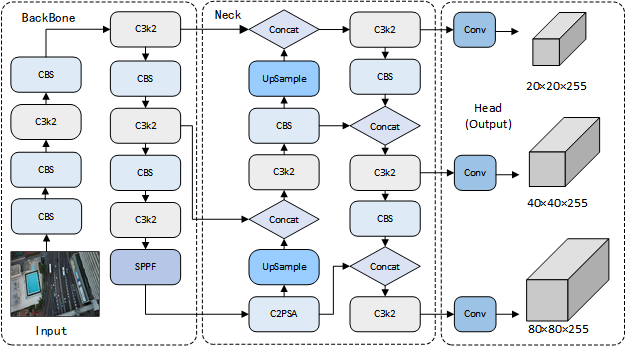
\includegraphics[width=0.8\linewidth]{../figure/yolov11.png}
%     }
%     \captionsetup{font=footnotesize}
%     \bicaption{GAN 网络结构框架}{YOLOv11 network structure diagram.}
%     \label{fig:gan}
% \end{figure}

\begin{figure}[htb]
    \centering
    \subfloat{
    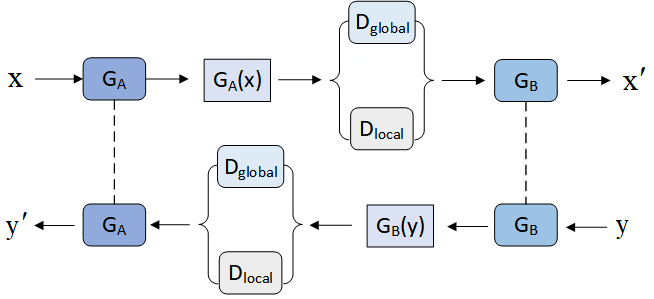
\includegraphics[width=0.8\linewidth]{../figure/cgan.png}
    }
    \captionsetup{font=footnotesize}
    \bicaption{CycleGAN 网络}{CycleGAN Net}
    \label{fig:cgan}
\end{figure}

GAN 通常需要大量的成对数据进行训练,这在许多实际应用中是一个巨大的挑战。例如,在去雾还原任务中,获取大量成对的有雾图像和对应的无雾图像是非常困难的,因为无雾图像往往难以直接获得,或者需要在特定条件下拍摄,这限制了 GAN 在该领域的应用。而 CycleGAN 则可以在无监督的情况下进行训练,即不需要成对的图像数据。它利用循环一致性约束,在只有两个不同域的非配对图像集合的情况下,学习图像之间的映射关系,这大大降低了数据获取的难度,为去雾还原等任务提供了更灵活的解决方案。

GAN 的网络结构相对简单,主要由一个生成器和一个判别器组成。生成器的目标是将随机噪声生成逼真的样本,判别器则用于区分生成样本和真实样本。GAN 的训练目标主要是通过最小化对抗损失函数,使生成器生成的样本尽可能接近真实数据分布,判别器尽可能准确地辨别真假样本。
CycleGAN 的网络结构更为复杂,包含两个生成器和两个判别器。其训练目标不仅包括对抗损失,还包括循环一致性损失。对抗损失确保生成器生成的图像在目标域中具有逼真的外观,而循环一致性损失则保证图像在转换过程中内容的完整性。这种双重约束机制使得 CycleGAN 能够在没有成对数据的情况下,学习到更稳定、更准确的图像转换映射关系。

\subsubsection{生成器网络}

%% 介绍 编码器 - 解码器 结构

CycleGAN是一种用于无监督图像到图像翻译的生成对抗网络架构。其生成器是整个网络的核心组件之一,主要承担着将输入图像从一个域(如雾天图像域)映射到目标域(如无雾图像域)的关键任务。生成器的目标是学习输入图像与目标图像之间的复杂非线性映射关系,使得生成的图像在视觉效果和语义信息上尽可能接近真实的目标域图像,从而实现图像的去雾还原等操作。

CycleGAN 的生成器通常采用编码器 - 解码器结构作为基础框架。生成器网络结构如图 \ref{fig:gnet} 所示。编码器部分负责将输入图像逐步下采样,提取图像的多尺度特征。例如,在处理一张雾天图像时,编码器通过一系列卷积层和池化层操作,将图像的空间分辨率降低,同时增加特征图的通道数。这一过程能够捕捉到图像中的局部和全局特征,如雾天图像中的物体轮廓、颜色分布等信息。这些特征对于后续的图像生成至关重要,因为它们包含了生成无雾图像所需的关键语义信息。

解码器部分则与编码器相反,它将编码器提取到的特征逐步上采样,恢复图像的空间分辨率。在上采样过程中,解码器通过转置卷积等操作,将低分辨率的特征图逐步放大,最终生成与输入图像尺寸相同的输出图像。这个过程需要合理地利用编码器提取的特征,以确保生成的图像具有清晰的结构和细节。

\begin{figure}[htb]
    \centering
    \subfloat{
    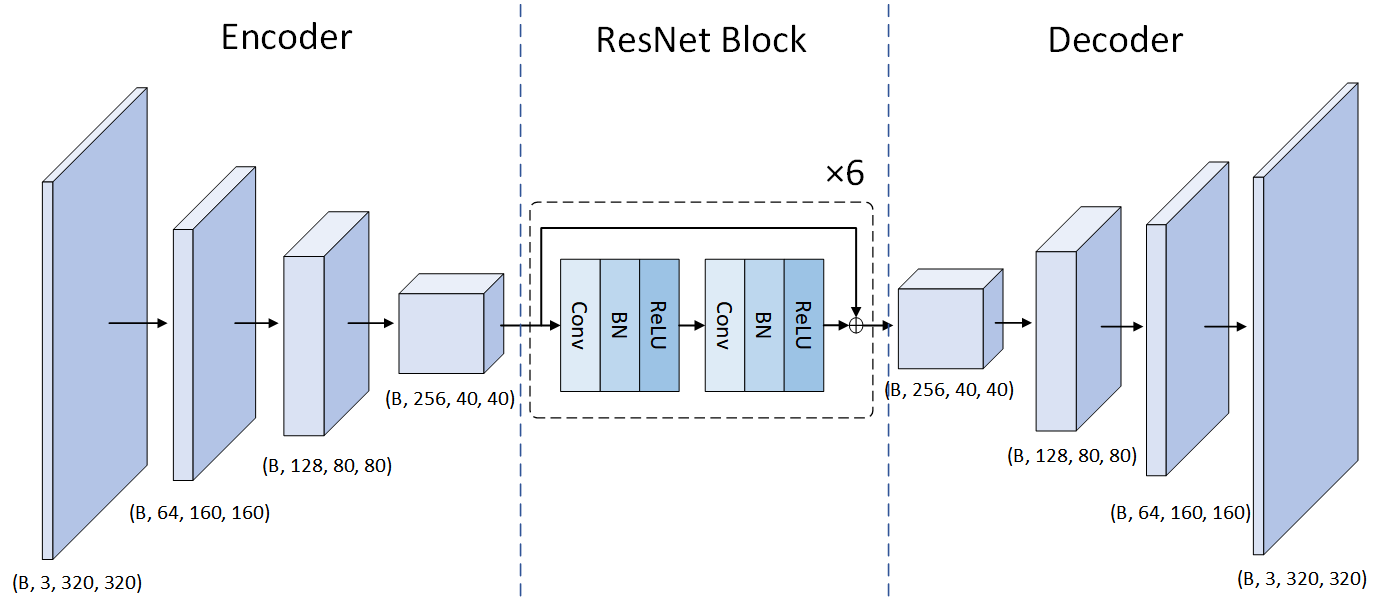
\includegraphics[width=1.0\linewidth]{../figure/generator.png}
    }
    \captionsetup{font=footnotesize}
    \bicaption{生成器网络}{Generator Net}
    \label{fig:gnet}
\end{figure}

%% 介绍ResNet残差块

为了提高生成器的性能,CycleGAN 在编码器 - 解码器结构中加入了残差块。残差块是深度残差网络(ResNet)中的重要组成部分,其核心思想是通过引入 shortcut connection(捷径连接)来缓解深层网络训练中的梯度消失问题。在生成器中,残差块使得网络能够更容易地学习到输入与输出之间的残差映射,而不是直接学习原始映射。

例如,在图 \ref{fig:gnet} 中,在生成器的中间部分,多个残差块可以堆叠在一起。每个残差块包含两个卷积层和一个 ReLU 激活函数。输入特征先进入第一个卷积层进行卷积操作,然后通过 ReLU 激活函数引入非线性,接着进入第二个卷积层。最后,将第二个卷积层的输出与输入特征相加,得到残差块的输出。这种设计使得网络在训练过程中能够更有效地传播梯度,从而能够构建更深的生成器网络,以捕捉更复杂的图像特征和映射关系。

%% 卷积与反卷积

\begin{figure}[htb]
    \centering
    \subfloat{
    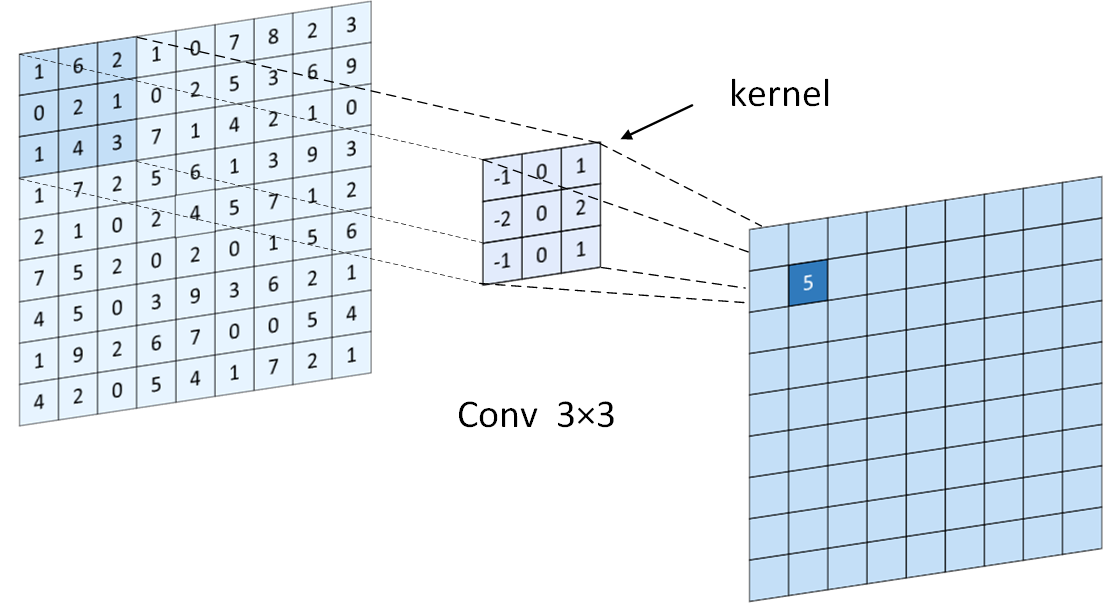
\includegraphics[width=0.7\linewidth]{../figure/conv_detail.png}
    }
    \captionsetup{font=footnotesize}
    \bicaption{卷积网络模块}{Conv Module}
    \label{fig:conv_detail}
\end{figure}

\begin{figure}[htb]
    \centering
    \subfloat{
    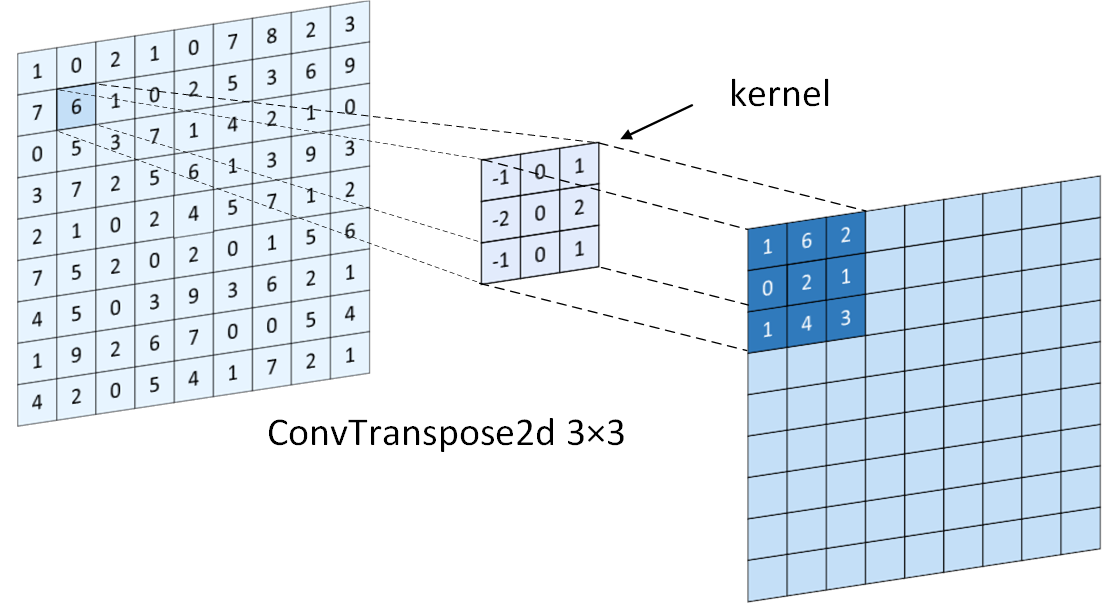
\includegraphics[width=0.7\linewidth]{../figure/convtranspose.png}
    }
    \captionsetup{font=footnotesize}
    \bicaption{反卷积网络模块}{Convtranspose Module}
    \label{fig:convtranspose}
\end{figure}

卷积层是生成器中的基础组件,用于提取图像的局部特征。在编码器部分,卷积层通过卷积核在图像上滑动,进行加权求和操作,提取图像的边缘、纹理等特征。卷积层的输出通道数通常会逐渐增加,以捕捉更丰富的特征信息。
反卷积层(或转置卷积层)在解码器部分用于上采样操作,将低分辨率的特征图逐步放大。反卷积层通过学习卷积核的反向操作,将特征图的空间分辨率提高,从而恢复图像的细节。在反卷积过程中,合理的参数设置和初始化对于生成图像的质量至关重要。卷积层和反卷积层网络结构如图 \ref{fig:conv_detail}、\ref{fig:convtranspose} 所示。


\subsubsection{判别器网络}

全局判别器在整个图像层面进行判断,关注图像的整体特征和分布。它接收完整的图像作为输入,通过多层卷积操作提取图像的全局特征,包括图像的整体结构、颜色分布、纹理模式等宏观信息。其主要作用是判断输入图像是否符合目标域图像的整体特征分布,确保生成图像在整体上具有真实图像的外观和风格。例如,在去雾任务中,全局判别器会学习雾天图像和清晰图像在整体上的差异,如雾天图像通常具有较低的对比度、偏白的颜色倾向以及模糊的轮廓等特征,从而指导生成器生成具有清晰结构、自然颜色分布和高对比度的去雾图像。

全局判别器通常采用卷积神经网络结构,判别起网络结构如图 \ref{fig:dnet} 所示。包含多个卷积层、激活函数层(如 Leaky ReLU)以及池化层。输入图像经过卷积层的逐层特征提取,图像的空间尺寸逐渐减小,而特征通道数逐渐增加,最终得到一个特征向量。该特征向量被送入全连接层,输出一个概率值,表示输入图像属于目标域真实图像的概率。在训练过程中,全局判别器与生成器进行对抗训练。生成器试图生成能够欺骗全局判别器的图像,使其误认为生成图像是真实图像;而全局判别器则不断学习如何更准确地区分真实图像和生成图像,通过梯度下降更新网络参数,优化判别性能。这种对抗训练过程促使生成器不断提升生成图像的整体质量,使其在全局特征上逐渐接近真实图像的分布。

\begin{figure}[htb]
    \centering
    \subfloat{
    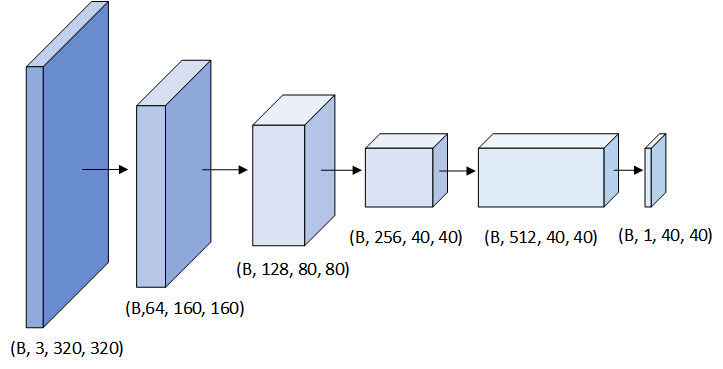
\includegraphics[width=0.8\linewidth]{../figure/discriminator.png}
    }
    \captionsetup{font=footnotesize}
    \bicaption{判别器网络}{Discriminator Net}
    \label{fig:dnet}
\end{figure}

%% 全局判别器

全局判别器在去雾过程中发挥着关键作用。它能够确保去雾后的图像在整体上具有清晰、自然的视觉效果,避免出现整体结构失真或颜色偏差等问题。例如,当生成器生成的去雾图像整体对比度较低或颜色偏暗时,全局判别器会给出较低的真实性概率,从而促使生成器调整生成策略,提高去雾图像的整体质量。通过全局判别器的监督,生成器能够生成符合清晰图像全局特征的去雾结果,增强去雾图像的视觉吸引力和可用性。

局部判别器聚焦于图像的局部区域,关注图像的细节特征和局部纹理。它通过随机裁剪或采样等方法获取图像的局部小块区域作为输入,对这些局部区域进行判别。其主要作用是确保生成图像在局部细节上具有真实图像的纹理和结构特征,避免生成图像出现模糊、失真或不合理的局部图案。在去雾任务中,局部判别器能够帮助生成器恢复图像中被雾气遮挡的细节信息,如物体的边缘、纹理等,使去雾后的图像在局部区域更加清晰、真实。

局部判别器的网络结构与全局判别器类似,也是基于 CNN 构建。由于其输入是图像的局部小块区域,因此网络的层数和参数量相对较少。局部判别器对输入的局部区域进行卷积操作,提取局部特征,如边缘、纹理、局部颜色过渡等细节信息。经过多层卷积和激活函数处理后,输出一个概率值,表示该局部区域属于目标域真实图像对应局部区域的概率。在训练过程中,局部判别器同样与生成器进行对抗训练。生成器需要生成在局部细节上逼真的图像,以欺骗局部判别器;而局部判别器则不断学习如何更准确地辨别局部区域的真实性。这种对抗训练使得生成器在生成图像时更加注重局部细节的还原和真实感,提高了去雾图像的细节质量。

%% 局部判别器

局部判别器对于去雾效果的提升主要体现在图像细节的恢复和增强方面。在雾天图像中,物体的边缘和纹理往往被雾气模糊,细节信息丢失严重。局部判别器能够指导生成器在去雾过程中有效地恢复这些局部细节,使去雾后的图像能够呈现出物体清晰的轮廓和丰富的纹理。例如,对于建筑物的窗户、树叶的脉络等细节部位,局部判别器可以促使生成器生成更加精细、真实的细节,从而提高去雾图像的整体质量和视觉效果。同时,局部判别器还有助于避免生成图像出现局部失真或不合理的人工痕迹,确保去雾图像的自然性和可信度。


全局判别器和局部判别器在 CycleGAN 的去雾还原算法中相互补充、协同作用。全局判别器从整体上把握图像的宏观特征和风格,确保生成图像在整体布局、颜色分布等方面符合清晰图像的要求;局部判别器则专注于图像的细节部分,保证生成图像在局部区域具有真实的纹理和结构。在训练过程中,生成器需要同时满足全局判别器和局部判别器的要求,既要生成具有真实整体特征的图像,又要在局部细节上做到逼真自然。这种协同作用使得生成器能够生成高质量、高保真的去雾图像,有效地解决了图像去雾中的细节恢复和整体质量提升的难题。例如,在处理一幅包含复杂场景的雾天图像时,全局判别器确保整个场景的清晰度和自然度,如天空的蓝色、地面的颜色分布等;局部判别器则负责恢复场景中物体的细节,如人物的面部表情、车辆的标志等,从而使最终的去雾图像在整体和局部都达到较好的效果。

\subsection{优化的CycleGAN网络}

\subsubsection{Transformer模块}

随着深度学习的蓬勃发展,Transformer 架构在众多领域大放异彩。它最初在自然语言处理任务中取得突破性成果,如今也将其强大的学习能力拓展至图像处理领域。在基于 CycleGAN 的去雾还原算法中,将 Transformer 插入生成器网络,可显著提升对复杂去雾还原问题的学习效果,这源于 Transformer 独特且精妙的结构与机理。

Transformer 主要由编码器和解码器两部分构成,在一些图像相关任务的变体架构中,会根据实际需求对这两部分进行适当调整或简化。

%% Transformer

Transformer 的编码器通过多层堆叠结构(含多头自注意力机制与位置前馈网络子层),将输入数据转换为富含语义信息的中间表示。在去雾任务中,多头自注意力机制分析像素关联,把握图像结构;位置前馈网络提升模型表达力,助力学习复杂特征。
解码器结合编码器输出和目标序列先验信息生成去雾图像,其多层结构含掩码多头自注意力、多头注意力及位置前馈子层。掩码机制确保生成顺序性,多头注意力促进编码器与解码器间信息交互。
自注意力机制作为 Transformer 核心,通过查询、键、值向量计算元素关联权重,多头注意力并行运行多个自注意力头,增强模型表达与特征捕捉能力。位置编码(如正弦、余弦或可学习嵌入)弥补自注意力对位置信息的忽视,助力模型理解元素顺序。

本文提出一种基于 Transformer 改进的 Transformer 模块,巧妙地嵌入到基于 CycleGAN 的去雾还原算法的生成器网络中,显著增强了生成器对去雾还原任务的学习效能。改进的 Transformer 网络结构如图 \ref{fig:transformer} 所示。

\begin{figure}[htb]
    \centering
    \subfloat{
    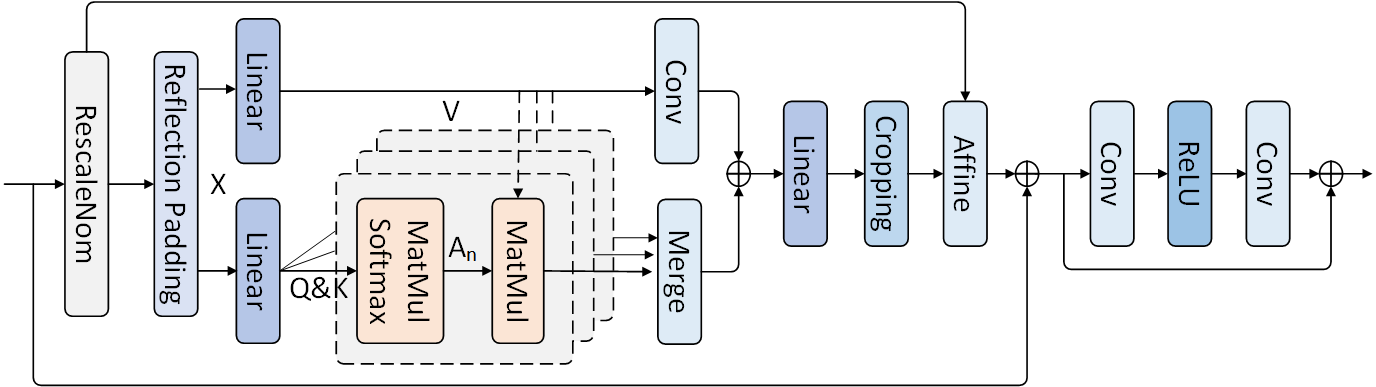
\includegraphics[width=1.0\linewidth]{../figure/transformer.png}
    }
    \captionsetup{font=footnotesize}
    \bicaption{改进的 Transformer 模块}{Improved Transformer Module}
    \label{fig:transformer}
\end{figure}

改进的 Transformer 模块由多个核心组件协同构成。输入特征 $x$ 经历两次主要的加工循环。第一次循环聚焦于注意力机制部分:
先经由 LayerNorm 进行规范化,此处规范操作能稳固特征的数值分布;
随后输入到注意力模块中,实现特征序列中各元素间关联性的捕捉与衡量;
对输出特征实施重缩放和再偏置,这类操作有助于恢复特征的合理数值范围与分布特性,避免因规范化带来的信息畸变;
最后,将加工后的特征与原始输入特征相加,完成残差连接操作,残差连接可确保梯度顺畅传导,缓解深层网络训练时的梯度消失问题,保障模型稳定学习。

假设输入特征为 $X \in R^{H \times W \times C} $,其中 $H$ 为高度,$W$ 为宽度,$C$ 为通道数。
首先应用 LayerNorm 对输入进行归一化,可以表示为:
\begin{equation}
    \label{eq:transformer1}
    X_{norm},\ rescale,\ rebias = LayerNorm(X)
\end{equation}

公式\ref{eq:transformer1}中,$X_{norm}$ 是归一化后的特征,$rescale$ 和 $rebias$ 分别是归一化模块输出的缩放参数和偏置参数。

然后将归一化后的特征输入到注意力机制模块 attn:
\begin{equation}
    X_{attn} = attn(X_{norm})
\end{equation}

对注意力输出进行缩放和偏置调整:
\begin{equation}
    X_{attn\_scaled} = X_{attn} \times rescale + rebias
\end{equation}

最后与残差连接相加:
\begin{equation}
    X_{res} = X + X_{attn\_scaled}
\end{equation}

第二次循环则围绕多层感知机(mlp)展开:再次以输入特征为基准建立残差连接(identity);
特征输入到 mlp 模块,历经两层线性变换搭配激活函数,实现对特征的非线性映射与维度拓展再压缩,深度挖掘特征的内在规律;
最终,将处理后的特征与本次循环起始的残差相加,输出本轮 Transformer 模块加工后的特征,为后续网络层传递更为丰富、抽象且贴合任务需求的特征表示。

将经过注意力机制和残差连接后的特征 $X_{res}$ 输入到多层感知机模块 mlp:
\begin{equation}
    X_{mlp} = mlp(X_{res})
\end{equation}

而多层感知机模块 mlp 由两个卷积层和一个激活函数组成:
\begin{equation}
    mlp(x) = Conv(ReLU(Conv(x)))
\end{equation}

将多层感知机的输出与残差连接相加得到最终输出:
\begin{equation}
    X_{out} = X_{res} + X_{mlp}
\end{equation}

相较于标准 Transformer 模块,该改进版融入了诸多契合视觉任务,尤其是去雾还原任务的创新设计。
其一,引入的窗口注意力机制及其移位策略,完美平衡了计算效率与感受野范围,在处理高维图像特征时避免了计算资源的过度消耗,同时确保模型能捕捉到图像全局结构与局部细节特征,这对于去雾任务中需要精准还原物体边缘、纹理等细节信息极为关键;
其二,灵活的规范化与残差连接配置选项,使整个模块能依据不同网络深度、特征维度场景,精准调控特征处理流程,提升模型适应性与性能表现,在 CycleGAN 生成器的复杂架构中,能与其他组件如卷积层、上采样层等无缝协同,全方位强化生成器对雾天图像特征的学习、转换与还原能力,最终输出高质量、视觉逼真的去雾图像成果。

综上所述,该改进的 Transformer 模块凭借精心设计的多头注意力机制、多层感知机模块,搭配巧妙的规范化与残差连接策略,深度契合去雾还原任务需求。将其嵌入 CycleGAN 生成器网络后,能显著增强模型对雾天图像复杂特征的学习、关联挖掘与高质量还原能力,推动基于 GAN 架构的图像去雾技术迈向新高度,为众多依赖清晰图像输入的下游计算机视觉应用提供更优质的视觉数据基础。

\subsubsection{改进的生成器网络}

CycleGAN 的生成器常借助 ResNet 残差链接结构来实现图像到图像的转换任务 。虽 ResNet 残差结构助力 CycleGAN 在诸多图像生成场景下有着不错表现,但面对一些对细节捕捉要求极高且数据复杂多样的情况,其基于传统卷积的特征提取与转换能力稍显不足,难以充分挖掘并利用图像深层复杂关联特征,一定程度上制约了生成图像的质量提升以及模型在更高端任务中的拓展应用。鉴于此,本文创新性地提出将 Transformer block 巧妙插入到 CycleGAN 生成器的 ResNet 残差块结构之中。

Transformer block 插入后的残差块结构如图 \ref{fig:cganformer} 
所示。该结构在保留 ResNet 残差核心优势基础上,融合了 Transformer 的强大特性,主要由自注意力机制模块、前馈神经网络模块以及与原 ResNet 残差结构的融合连接模块构成。自注意力机制模块能够捕捉图像不同位置间全局依赖关系,突破传统卷积局部感受野限制,使模型精准聚焦于图像关键信息区域,深度理解图像语义。前馈神经网络模块则进一步对特征进行非线性变换,增强特征表达丰富度。融合连接模块保障新结构与原 ResNet 残差架构无缝衔接,既继承残差学习优势,又充分释放 Transformer 潜能。

\begin{figure}[htb]
    \centering
    \subfloat{
    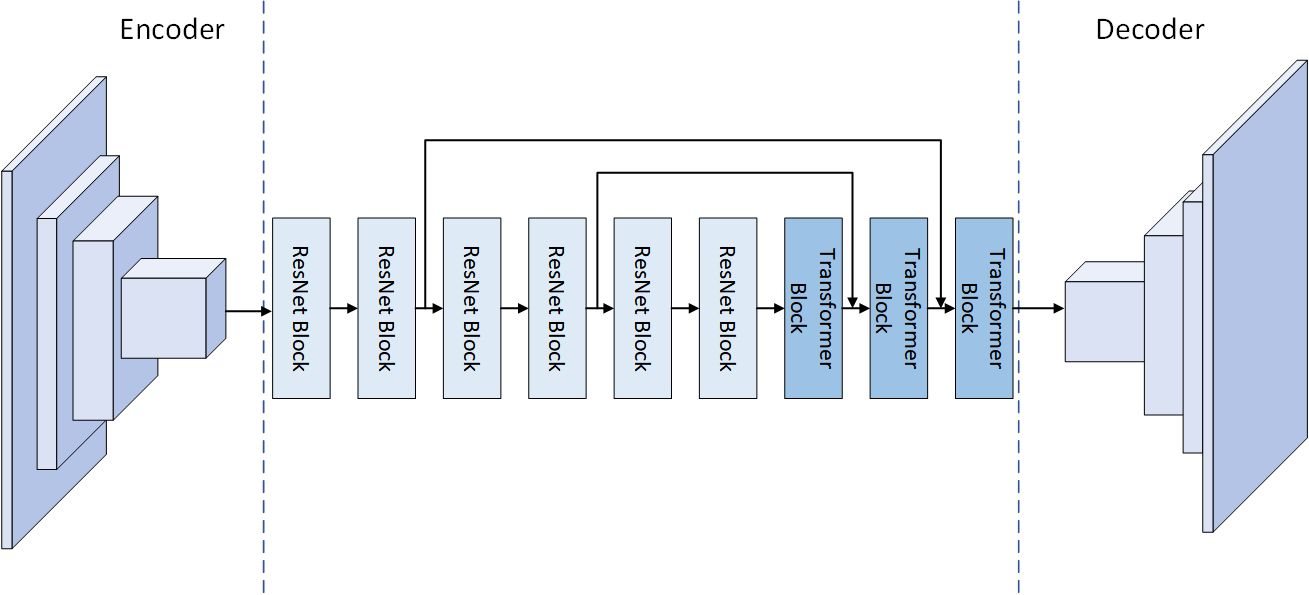
\includegraphics[width=1.0\linewidth]{../figure/cganformer.png}
    }
    \captionsetup{font=footnotesize}
    \bicaption{改进的生成器网络}{YOLOv11 network structure diagram.}
    \label{fig:cganformer}
\end{figure}

ResFormerGenerator 生成器网络由编码器、残差块、Transformer 块和解码器组成。其结构设计遵循了典型的编码 - 解码架构,能够有效地提取和还原图像的多尺度特征。

在 ResFormerGenerator 中,共有 6 个残差块。残差块的设计目的是解决深度神经网络中的梯度消失问题,并促进信息的高效传递。每个残差块包含两个卷积层和一个跳跃连接(skip connection)。跳跃连接将输入直接传递到块的输出,使得网络可以更容易地学习残差映射。

为了增强生成器网络对全局特征的学习能力,ResFormerGenerator 引入了 3 个改进的 Transformer 块。Transformer 块最初在自然语言处理领域取得巨大成功,其核心思想是利用自注意力机制捕捉序列中元素之间的长距离依赖关系。在图像处理中,可以将图像视为像素序列,从而应用 Transformer 块。
每个 Transformer 块包含多头自注意力和多层感知机。多头自注意力通过计算查询(Query)、键(Key)和值(Value)向量之间的点积,得到注意力权重矩阵,进而对输入特征进行加权求和,从而捕捉全局上下文信息。

编码器将输入的雾天图像特征进行编码,提取出主要的图像特征向量。假设输入的雾天图像特征为 $X_{in} \in R^{H \times W \times C}$,其中 $H$、$W$ 分别是图像的高度和宽度,$C$ 是通道数。编码器由一系列卷积层、归一化层和激活函数构成。经过编码器处理后,得到编码后的特征表示为 $F_{enc} \in R^{H' \times W' \times C'}$ ,其中 $H'$、$W'$、$C'$分别是编码后特征的高度、宽度和通道数。编码过程可以表示为:
\begin{equation}
    \label{eq:rfg1}
    F_{enc} = Encoder(X_{in})
\end{equation}

在 ResNet 块阶段,共有 6 个 ResNet 块。每个 ResNet 块包含两个卷积层、归一化层和激活函数,以及一个残差连接。对于第 $i$ 个 ResNet 块($i$=1,2,...,6),其输入为 $F_{res_{i-1}}$,输出为 $F_{res_{i}}$ ​,处理过程如下:
\begin{equation}
    \label{eq:rfg2}
    F_{res_{i}} = ResNetBlock_i(F_{res_{i-1}})
\end{equation}

公式\ref{eq:rfg2}中,第 1 个 ResNet 块的输入为编码后的特征$F_{enc}$,即$F_{res_{0}}\ =\ F_{enc}$。经过6个ResNet块后,得到特征$F_{res_{6}}$。

在 Transformer 块阶段,共有 3 个 Transformer 块。对于第 $j$ 个 Transformer 块($j$=1,2,3),其输入为 $F_{trans_{j-1}} + F_{res_{8-2j}}$,输出为 $F_{trans_{j}}$ ​,处理过程如下:
\begin{equation}
    \label{eq:rfg3}
    F_{trans_j} = TransformerBlock(F_{trans_{j-1}} + F_{res_{8-2j}}) 
\end{equation}

公式\ref{eq:rfg3}中,第 1 个 Transformer 块的输入为$F_{res_6}$。

解码器将经过 Transformer 块处理后的特征 $F_{trans_3}$ 进行上采样和卷积等操作,逐步恢复图像的空间分辨率。解码器由一系列反卷积层、归一化层和激活函数构成。最终输出去雾还原后的图像特征 $X_{out} \in R^{H \times W \times C_{out}}$,其中 $C_{out}$ 是通道数。解码过程可以表示为:
\begin{equation}
    \label{eq:rfg4}
    X_{out} = Decoder(F_{trans_3})
\end{equation}


Transformer Block 中的自注意力机制能够捕捉特征图中不同位置之间的全局依赖关系,这对于理解雾气在图像中的分布具有重要意义。相比之下,传统的卷积操作由于其局部感受野的限制,难以有效捕捉全局信息。通过引入自注意力机制,模型能够更好地学习到雾气在图像中的分布规律,从而提升去雾效果。

在前向传播过程中,跳跃连接将前面残差块的输出与当前 Transformer 块的输出相加,这种设计能够更好地融合不同层次的特征信息。低层特征包含丰富的纹理细节,而高层特征则包含语义信息。通过跳跃连接,模型能够综合利用不同层次的特征,生成更清晰、更自然的去雾图像。

\subsection{图像去雾实验和雾天目标检测实验结果和分析}

% 新算法 CGANFormer 在 NYU2\cite{nyu2}、Dense-Haze\cite{NTIRE_Dehazing_2019} 数据集上进行训练和测试图像去雾性能,以改进每个阶段。
% 在不同场景中选择复杂的场景图片,并将拟议算法的检测效果与实际场景中,并与 AODNet\cite{li2017aod}、FFA-Net\cite{ffa}、GCANet\cite{chen2019gated} 和 CycleGAN\cite{cgan} 算法进行比较。

% 最后将 CGANFormer 算法与 EX-YOLO算法结合,在FOG-TT100K、FOG-VisDrone数据集上进行雾天目标检测性能测试,并与YOLOv9s\cite{yolov9}、YOLOv10s\cite{yolov10}、YOLOv11s\cite{yolov11}算法进行比较。

新算法 CGANFormer 与 EX-YOLO算法结合,在FOG-TT100K、FOG-VisDrone数据集上进行雾天目标检测性能测试,并与YOLOv9s\cite{yolov9}、YOLOv10s\cite{yolov10}、YOLOv11s\cite{yolov11}算法进行比较。

% \subsubsection{数据集}

% NYU2 数据集是室内场景视觉研究领域的重要数据集,由纽约大学(NYU)构建。它包含 1449 对密集标注的 RGB 和深度图像,这些图像从多个城市的 464 个新场景中采集,利用微软 Kinect 的 RGB 和深度摄像机记录视频序列,还包含 407024 个新的未标注帧,为图像去雾等研究提供了大量室内场景的视觉数据资源,可用于训练和评估去雾算法在复杂室内环境中的性能。

% Dense-Haze 是一个用于图像去雾研究的高质量数据集,由 CVL 于 2019 年为 NTIRE 图像去雾挑战赛构建。该数据集包含 33 对真实雾气和无雾图像对,涵盖多样化的户外场景。这些图像对是在相同照明参数下,通过专业设备引入真实雾气生成技术拍摄的,具有高密度、均匀分布的雾气特征,旨在推动单图像去雾技术的发展。Dense-Haze 数据集不仅为去雾算法提供了可靠的评估基准,还通过综合定性和定量评估揭示了现有方法在处理密集均匀雾气场景时的局限性,为未来研究指明了改进方向。


\subsubsection{实验环境}

本文中用于实验的系统、系统硬件设施和软件平台如表\ref{tab:environment2}所示。
\begin{table}[htbp]
    \centering
    \captionsetup{font=footnotesize}
    \bicaption{实验环境设置}{Symbol cross-reference table}
    \label{tab:environment2}
    \begin{tabular}{>{\centering\arraybackslash}p{0.4\textwidth}>{\centering\arraybackslash}p{0.4\textwidth}}
        \toprule
        List              & Version            \\ 
        \midrule
        Operating System  & Ubuntu 22          \\
        Memory            & 64G RAM            \\
        CPU               & Intel i9-13900K    \\
        GPU               & NVIDIA GTX4090 GPU \\
        Cuda              & cu121              \\
        Python            & 3.11               \\
        \bottomrule
    \end{tabular}
\end{table}

\subsubsection{实验结果和分析}

% 在这项研究中,我们通过比较实验评估了 CGANFormer 模型(our)在2个不同数据集中,包括 NYU2 和 Dense-Haze 数据集上的性能,以验证图像去雾还原的改进方法的有效性。
% 通过将其与基准模型 CycleGAN、AODNet、FFA-Net、GCANet 进行比较,评估改进模型在各种指标上的性能。

% \begin{table}[htbp]
%     \centering
%     \captionsetup{font=footnotesize}
%     \bicaption{在 NYU2 数据集上的对比实验结果}{Symbol cross-reference table}
%     \label{tab:compare_studies_nyu2}
%     \begin{tabular}{p{0.13\textwidth}p{0.13\textwidth}p{0.13\textwidth}p{0.13\textwidth}p{0.13\textwidth}p{0.13\textwidth}}
%         \toprule
%         性能指标 & CycleGAN & AODNet & FFA-Net & GCANet & our   \\ 
%         \midrule
%         PSNR    & 9.5      & 21.8   & 0.877   & 0.878  & 0.777 \\
%         SSIM    & 8.2      & 25.4   & 0.850   & 0.776  & 0.752 \\
%         \bottomrule
%     \end{tabular}
% \end{table}

% \begin{table}[htbp]
%     \centering
%     \captionsetup{font=footnotesize}
%     \bicaption{在 Dense-Haze 数据集上的对比实验结果}{Symbol cross-reference table}
%     \label{tab:compare_studies_dh}
%     \begin{tabular}{p{0.13\textwidth}p{0.13\textwidth}p{0.13\textwidth}p{0.13\textwidth}p{0.13\textwidth}p{0.13\textwidth}}
%         \toprule
%         性能指标 & CycleGAN & AODNet & FFA-Net & GCANet & our   \\ 
%         \midrule
%         PSNR    & 9.5      & 21.8   & 0.877   & 0.878  & 0.777 \\
%         SSIM    & 8.2      & 25.4   & 0.850   & 0.776  & 0.752 \\
%         \bottomrule
%     \end{tabular}
% \end{table}


接下来比较我们通过比较实验评估了 CGF-YOLO模型(our)在2个不同数据集中,包括TT100K和VisDrone数据集上的性能,以验证小目标检测和多尺度目标检测的改进方法的有效性。
通过将其与基准模型YOLOv11s、YOLOv10s和YOLOv9s进行比较,评估改进模型在各种指标上的性能。

\begin{table}[htbp]
    \centering
    \captionsetup{font=footnotesize}
    \bicaption{在 FOG-TT100K 数据集上的对比实验结果}{Symbol cross-reference table}
    \label{tab:compare_studies_fogtt100k}
    \begin{tabular}{p{0.13\textwidth}p{0.13\textwidth}p{0.19\textwidth}p{0.1\textwidth}p{0.07\textwidth}p{0.07\textwidth}p{0.07\textwidth}}
        \toprule
        模型         & 图像大小 & 参数量 MB & 计算量 GFLOPs & $mAP_{0.5}$   & P     & R     \\%& FPS \\ 
        \midrule
        YOLOv11s     & 400     & 9.5     & 21.8          & 0.453        & 0.615  & 0.280 \\%& 94.3 \\
        YOLOv10s     & 400     & 8.2     & 25.4          & 0.414        & 0.570  & 0.249 \\%& 88.5 \\
        YOLOv9s      & 400     & 7.5     & 27.2          & 0.501        & 0.666  & 0.328 \\%& 90.9 \\
        \textbf{our} & 400     & 11.4    & \textbf{17.0} & 0.592        & 0.699  & 0.449 \\%& 84.7 \\
        \bottomrule
    \end{tabular}
\end{table}

\begin{figure}[htbp]
    \centering
        \subfloat[CGF-YOLO\label{fig:fogtt100k_ex_cmn}]{
            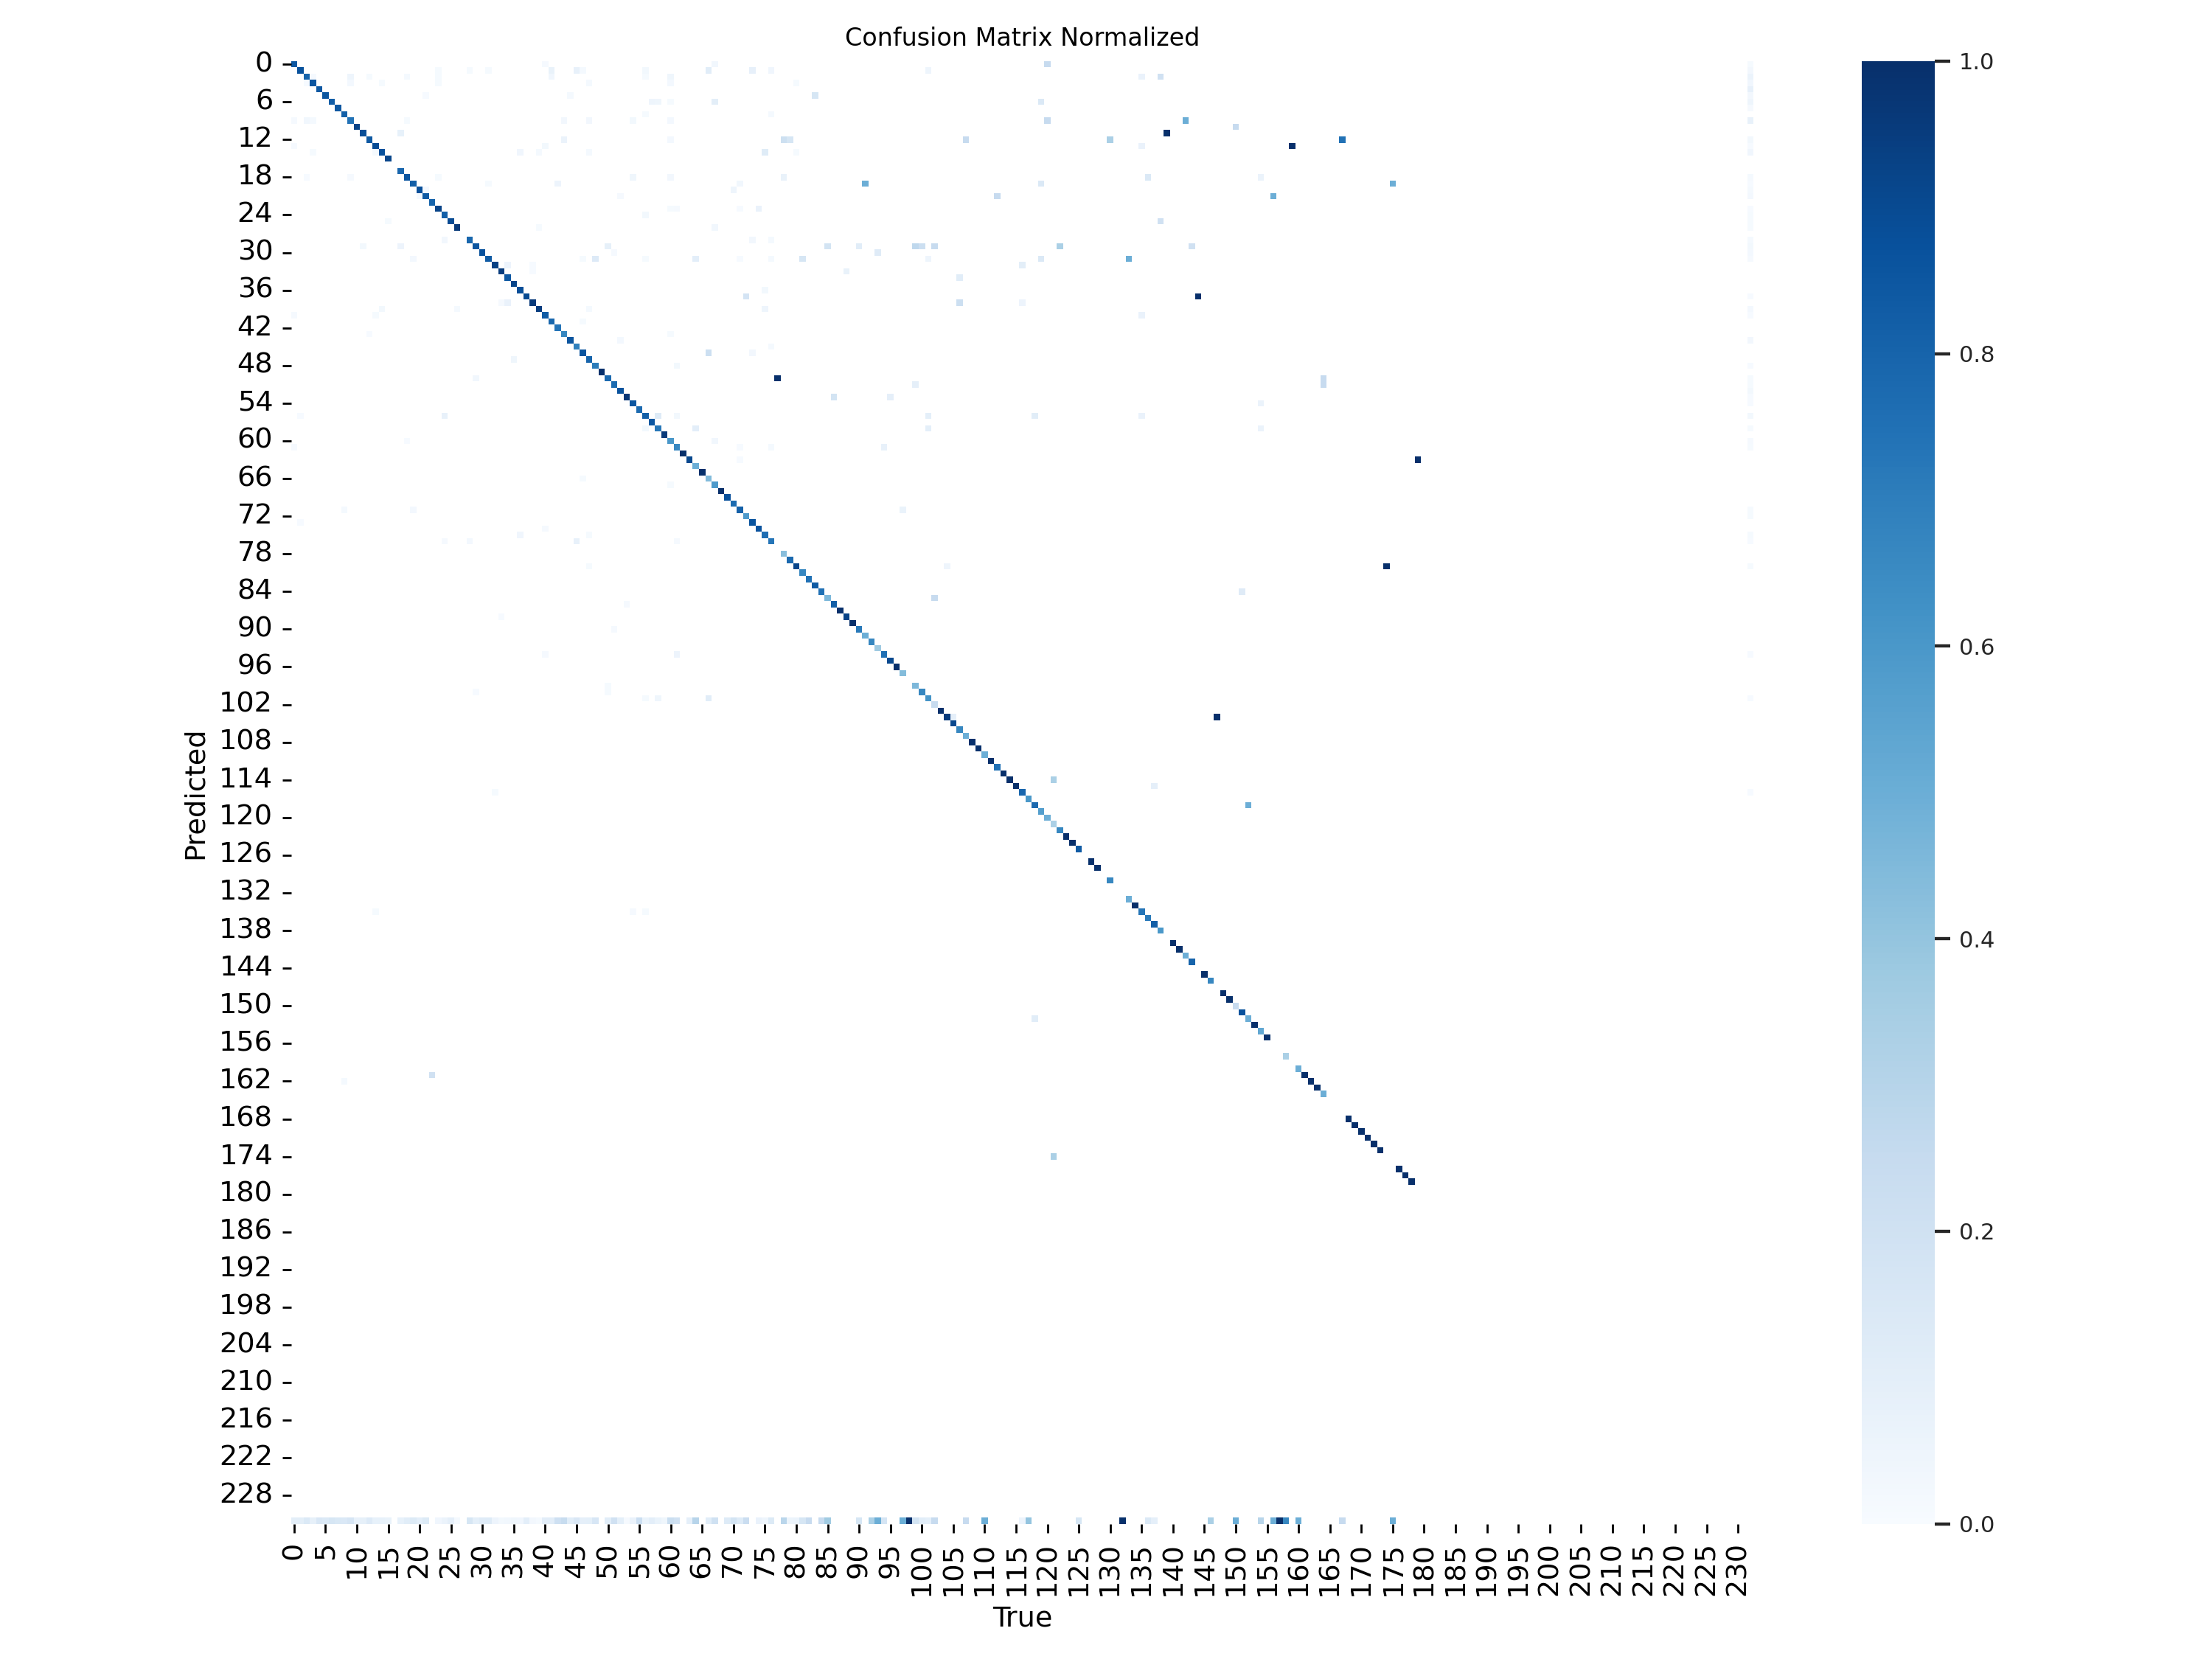
\includegraphics[width=0.4\textwidth]{../figure/tt100k_ex_confusion_matrix_normalized.png}
        }
        \subfloat[YOLOv11s\label{fig:fogtt100k_11s_cmn}]{
            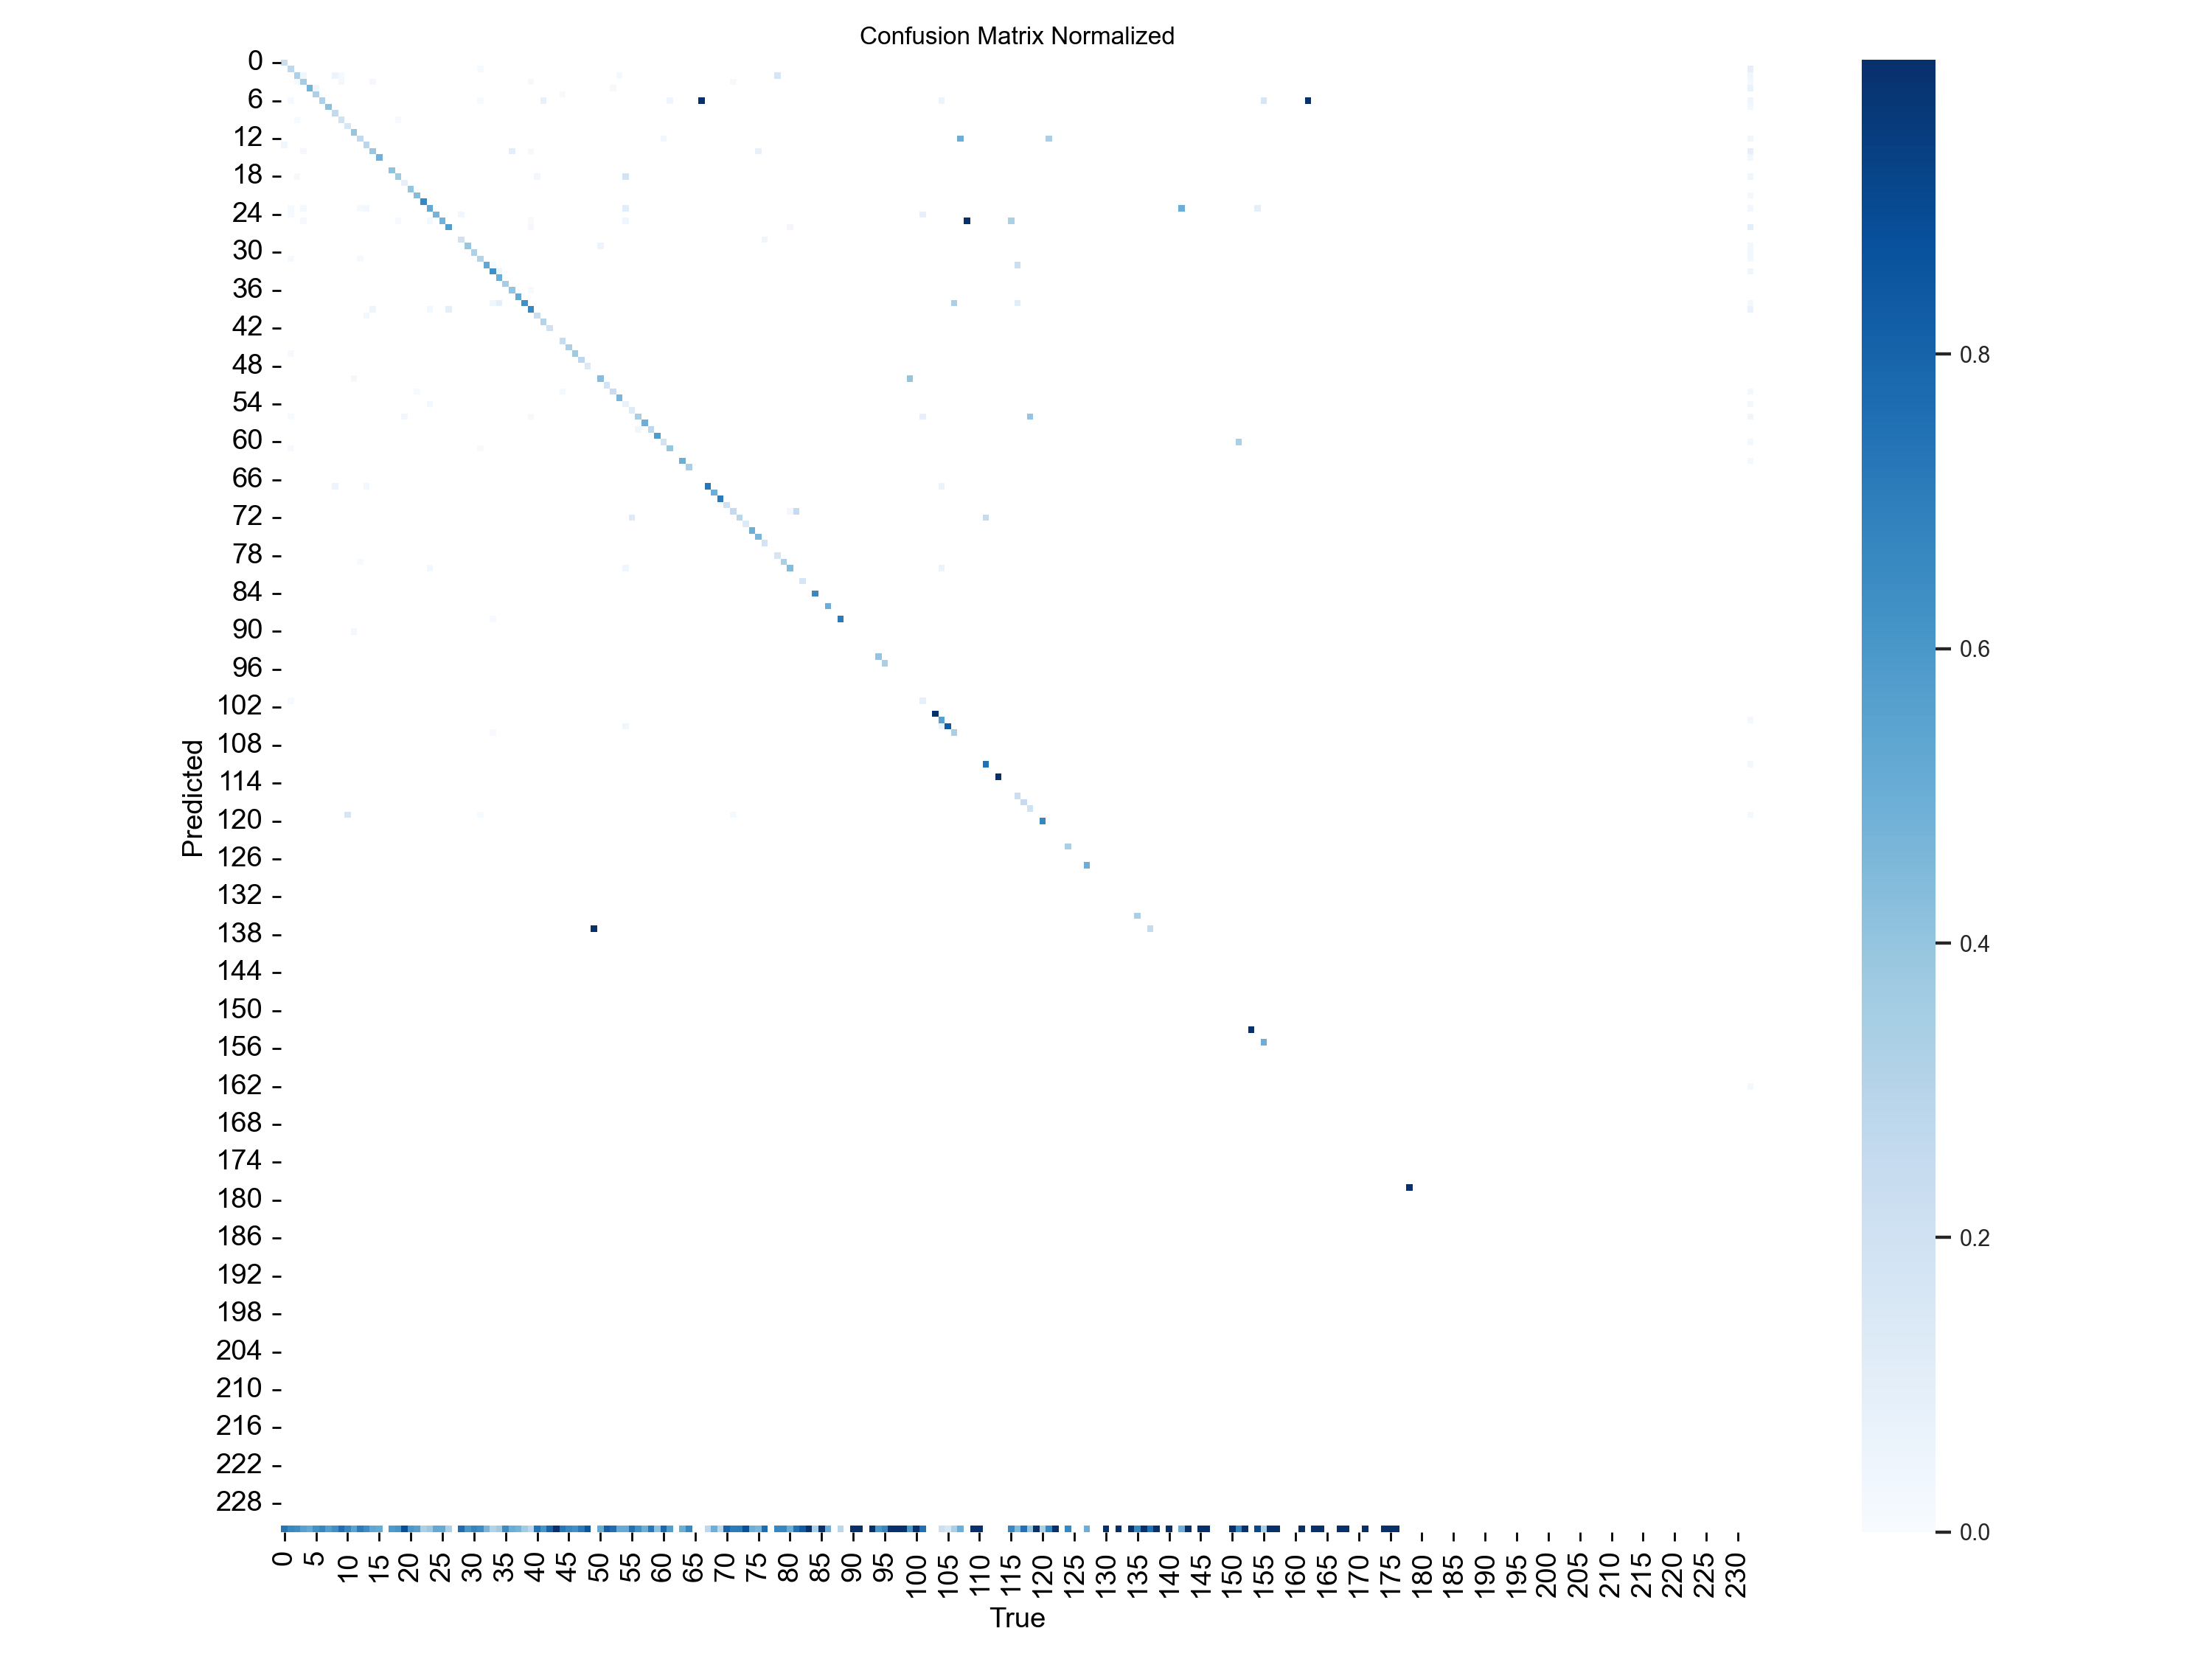
\includegraphics[width=0.4\textwidth]{../figure/fogtt_11_confusion_matrix_normalized.png}
        } \\
        \subfloat[YOLOv10s\label{fig:fogtt100k_10s_cmn}]{
            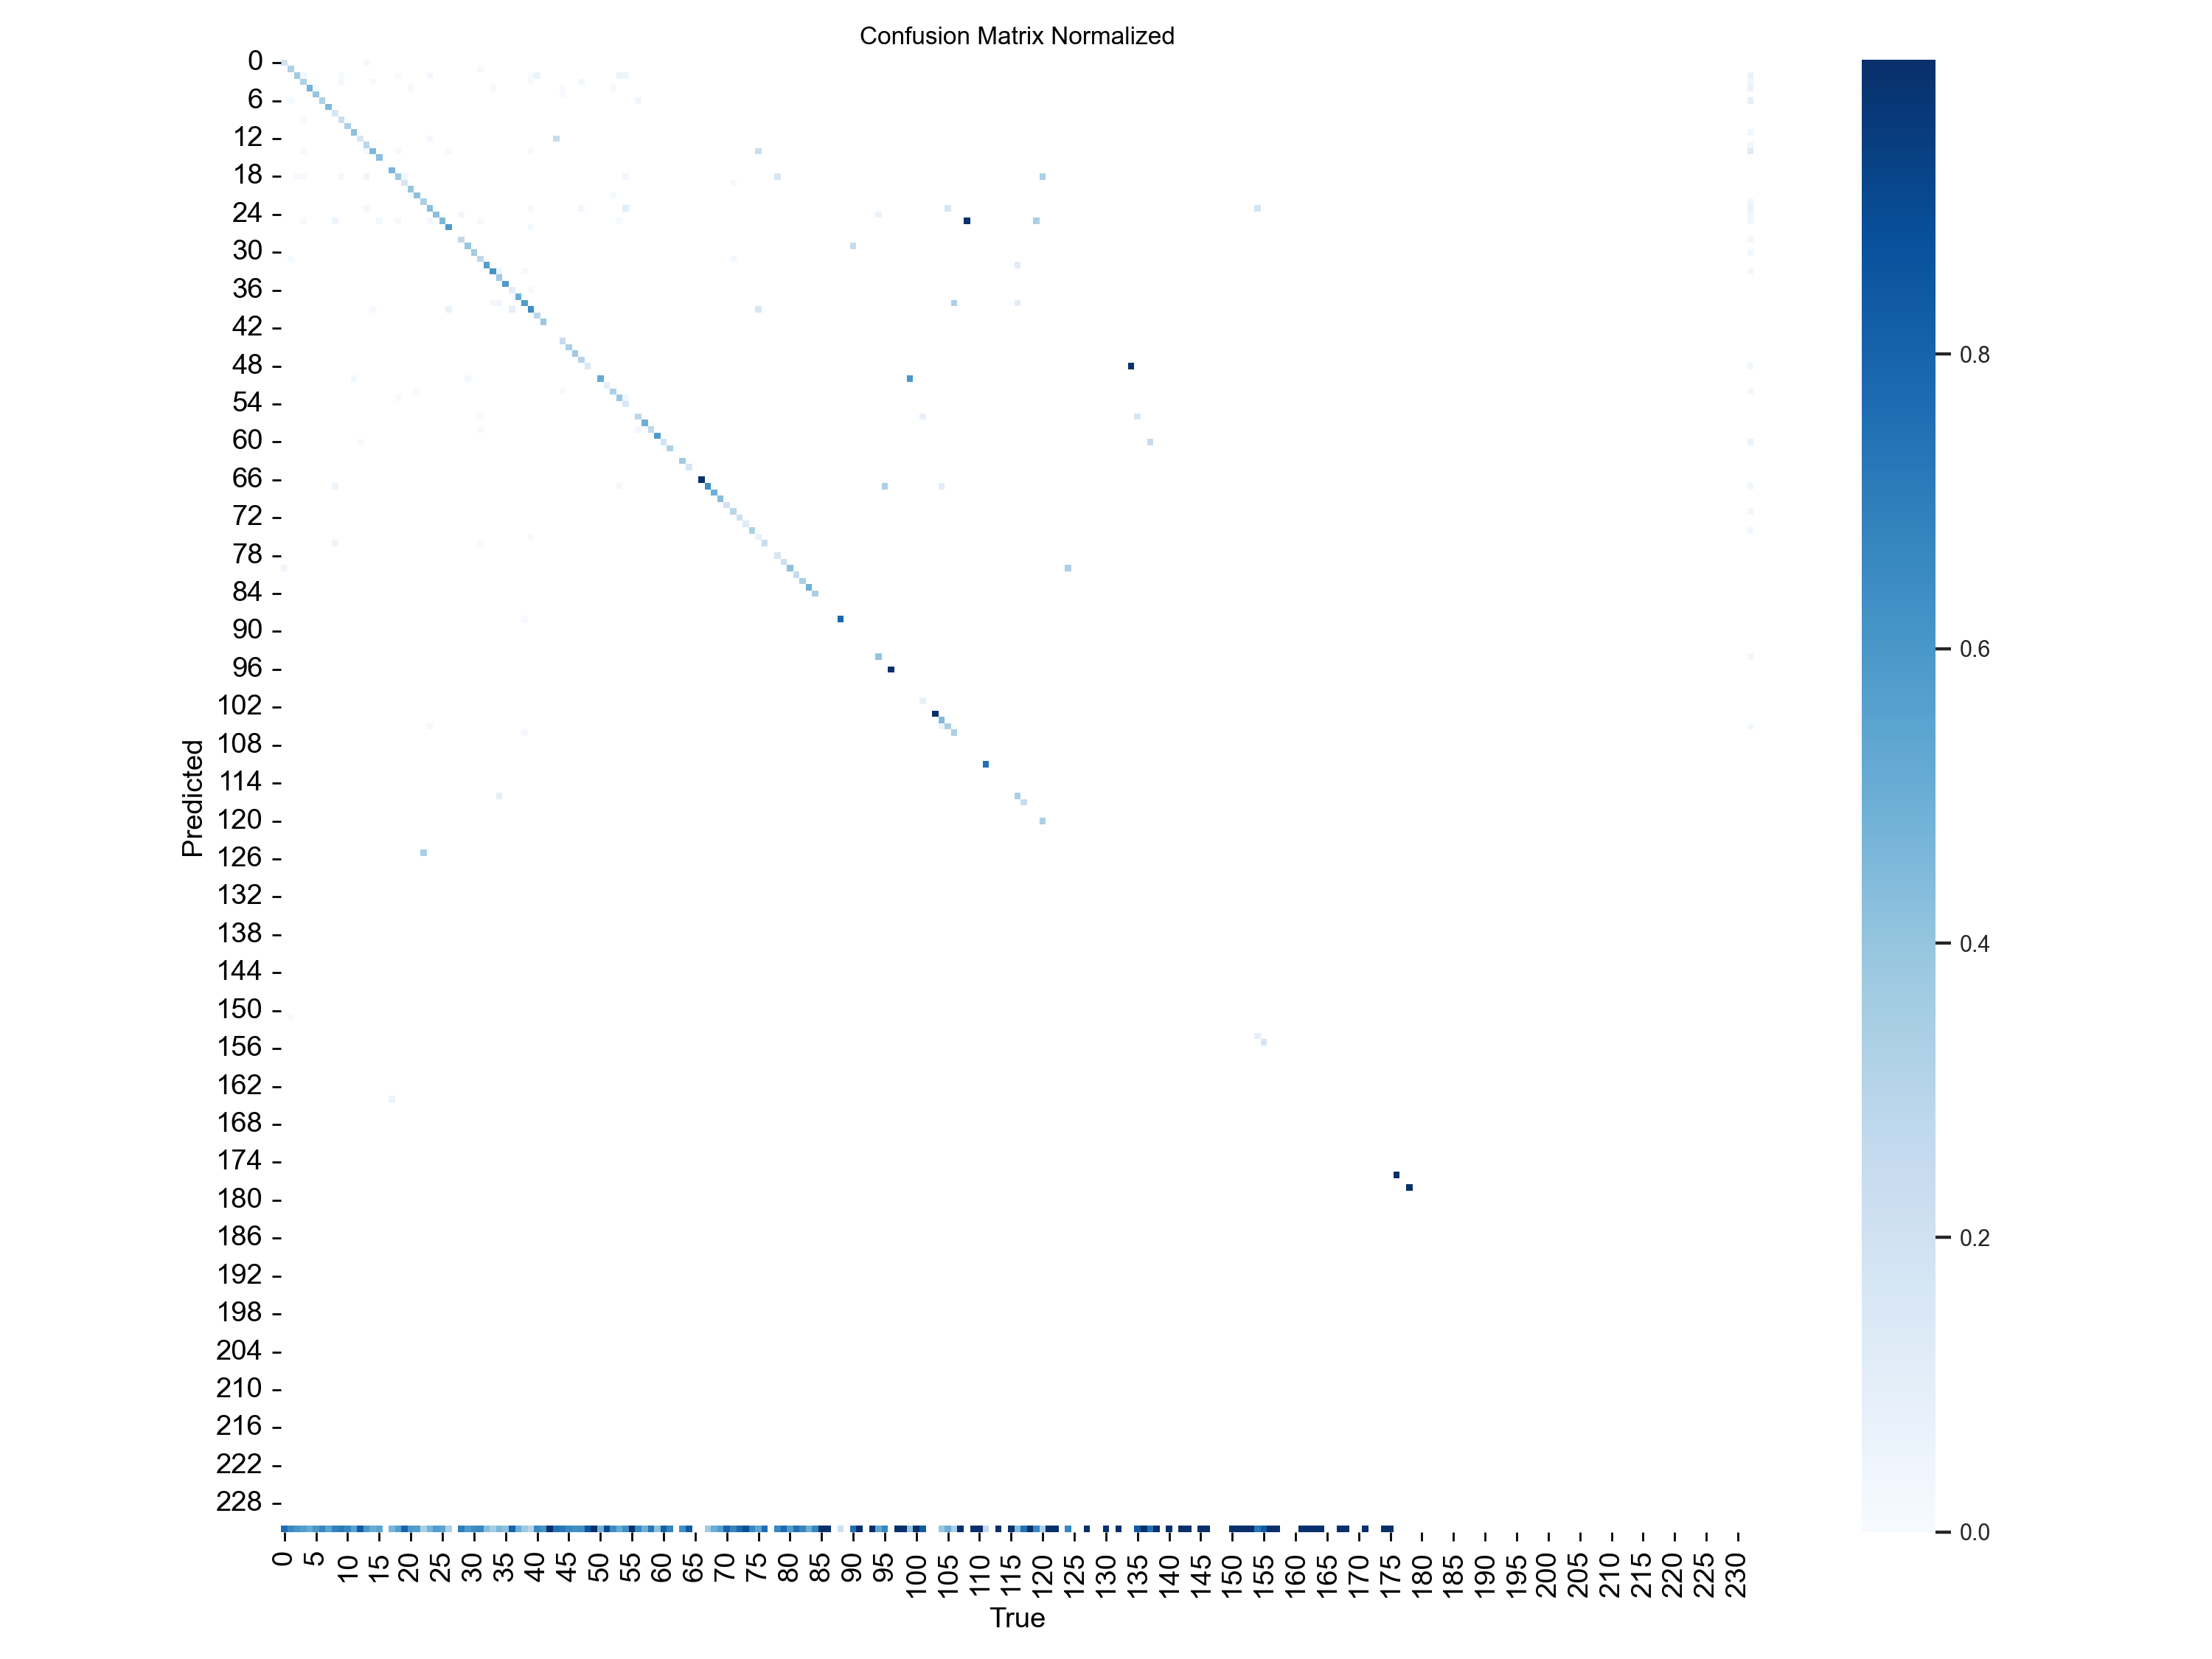
\includegraphics[width=0.4\textwidth]{../figure/fogtt_10_confusion_matrix_normalized.png}
        }
        \subfloat[YOLOv9s\label{fig:fogtt100k_9s_cmn}]{
            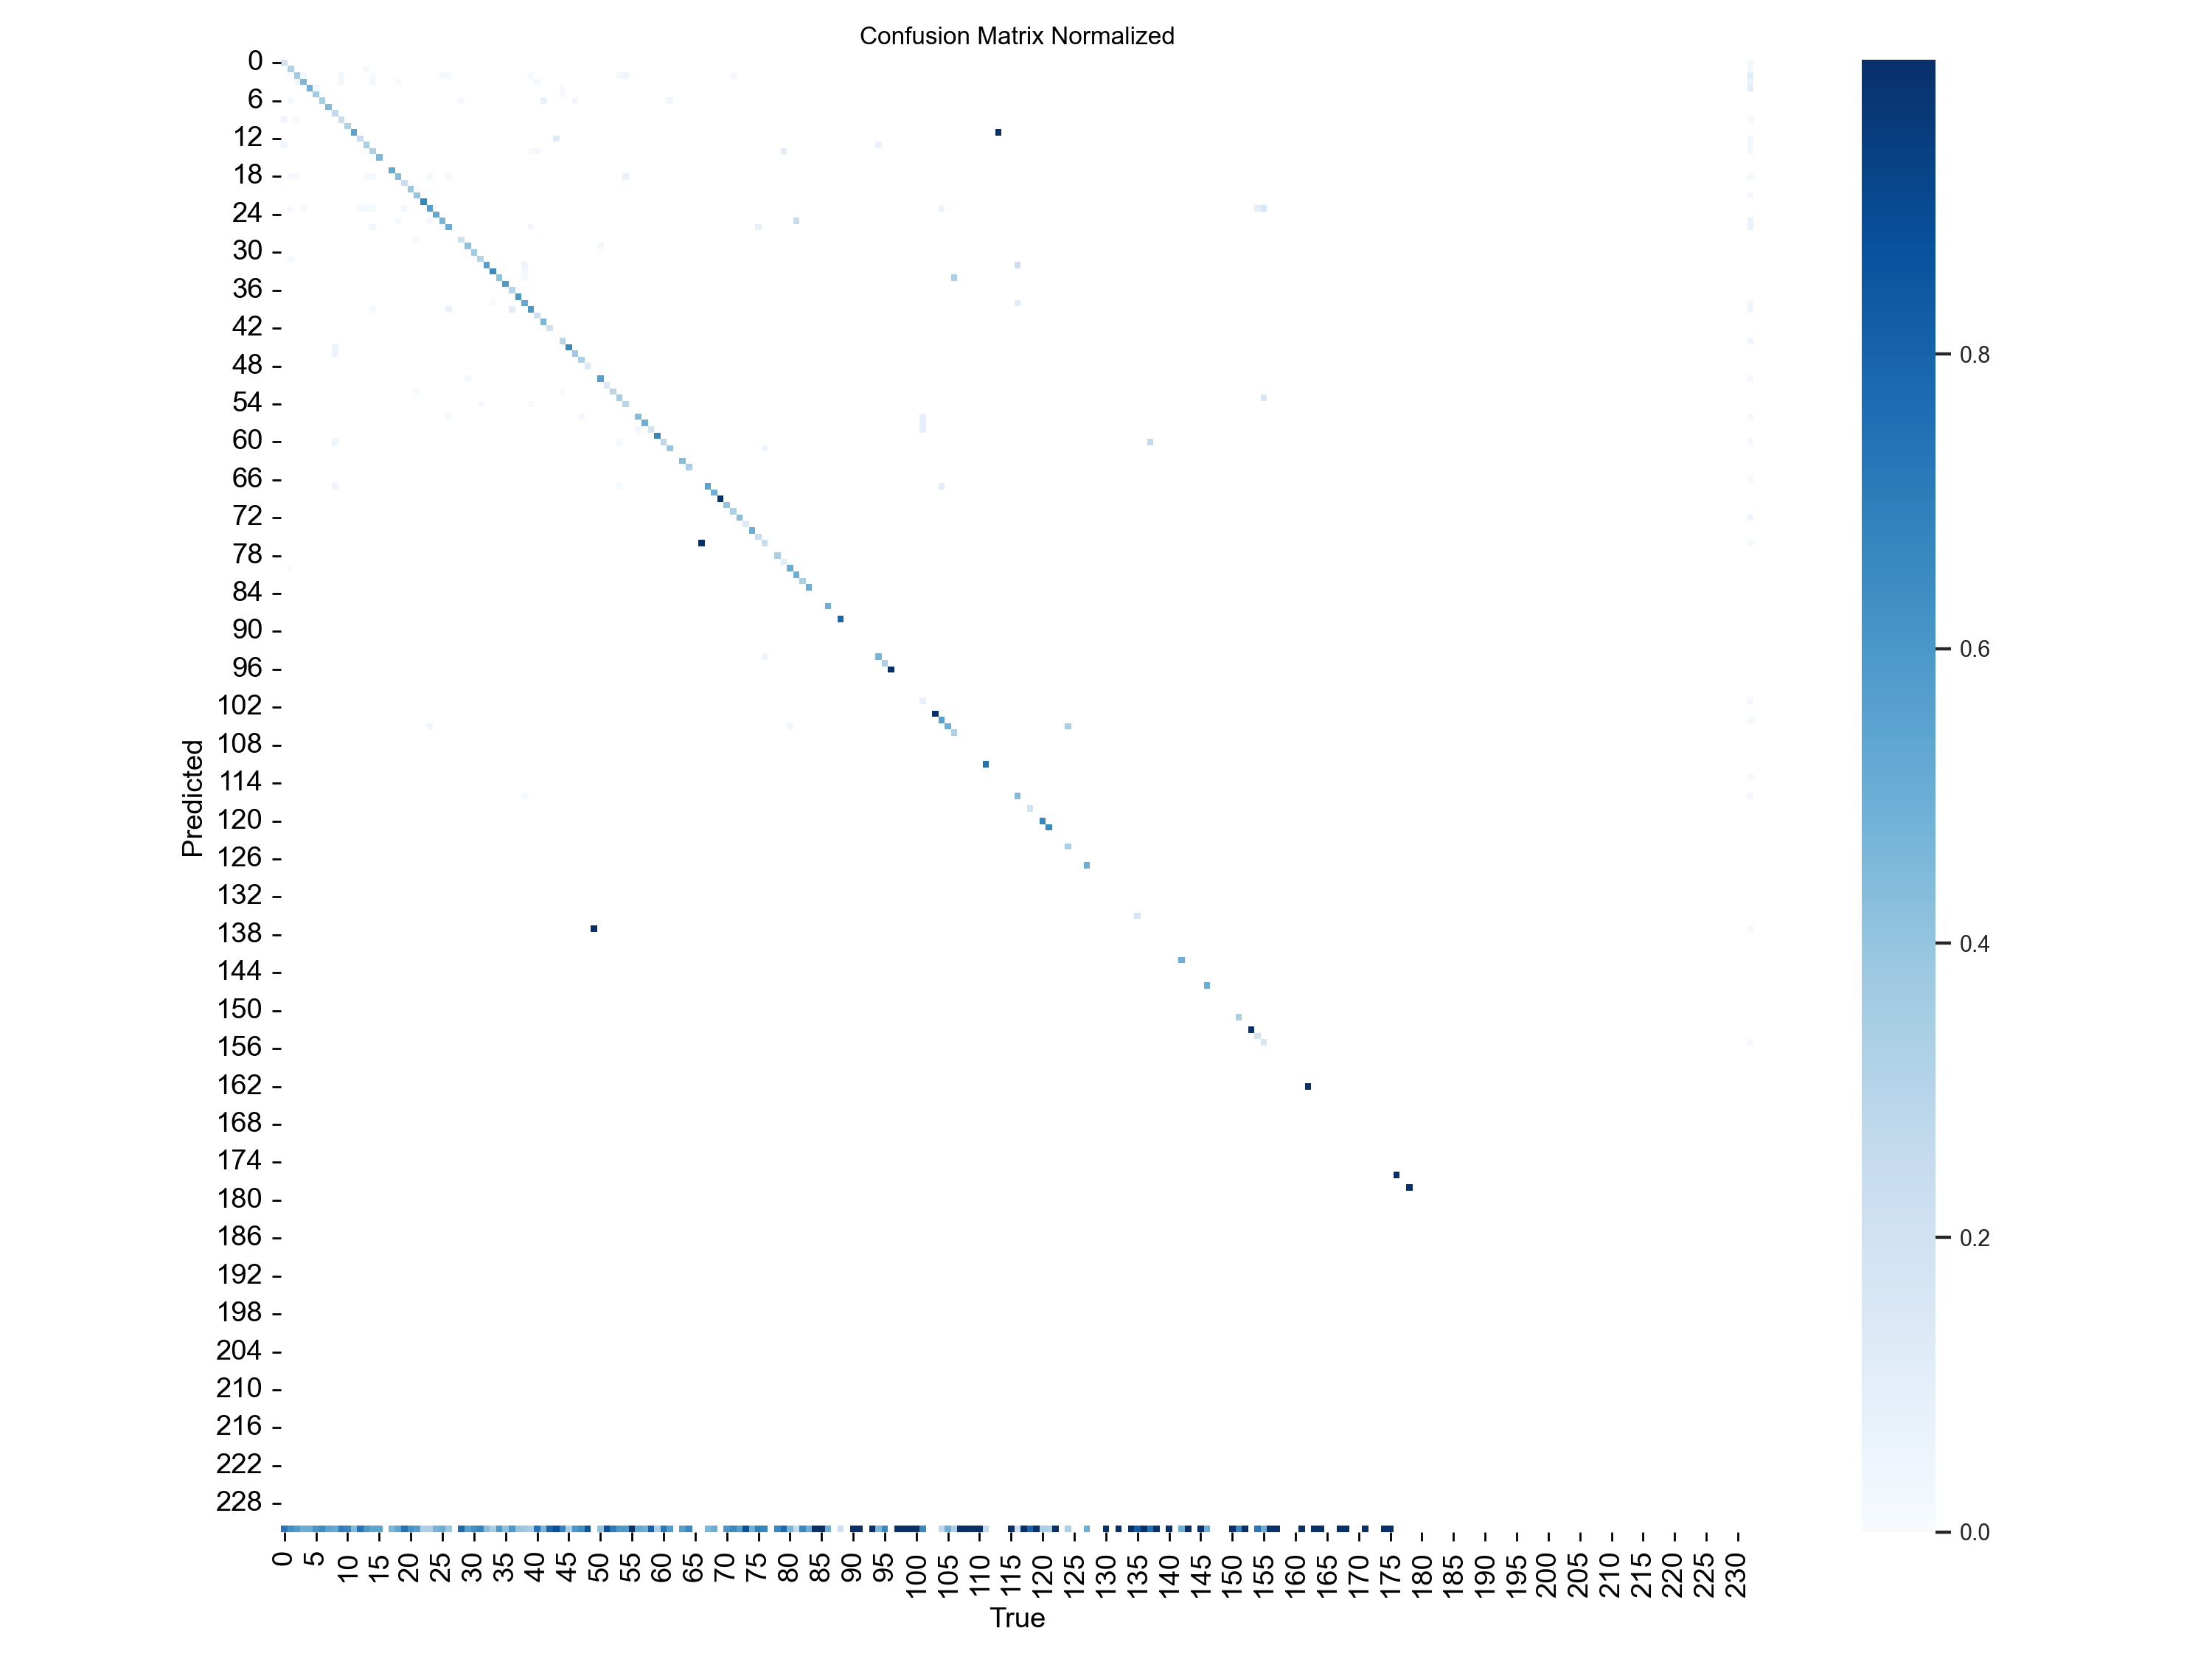
\includegraphics[width=0.4\textwidth]{../figure/fogtt_9_confusion_matrix_normalized.png}
        }
    \captionsetup{font=footnotesize}
    \bicaption{不同的网络模型在 FOG-TT100K 数据集上的归一化混淆矩阵}{The normalized confusion matrix of different network models on the FOG-TT100K dataset.}
    \label{fig:fogtt100k_cmn}
\end{figure}

\begin{figure}[htbp]
    \centering
        \subfloat[CGF-YOLO\label{fig:fogtt100k_ex_f1}]{
            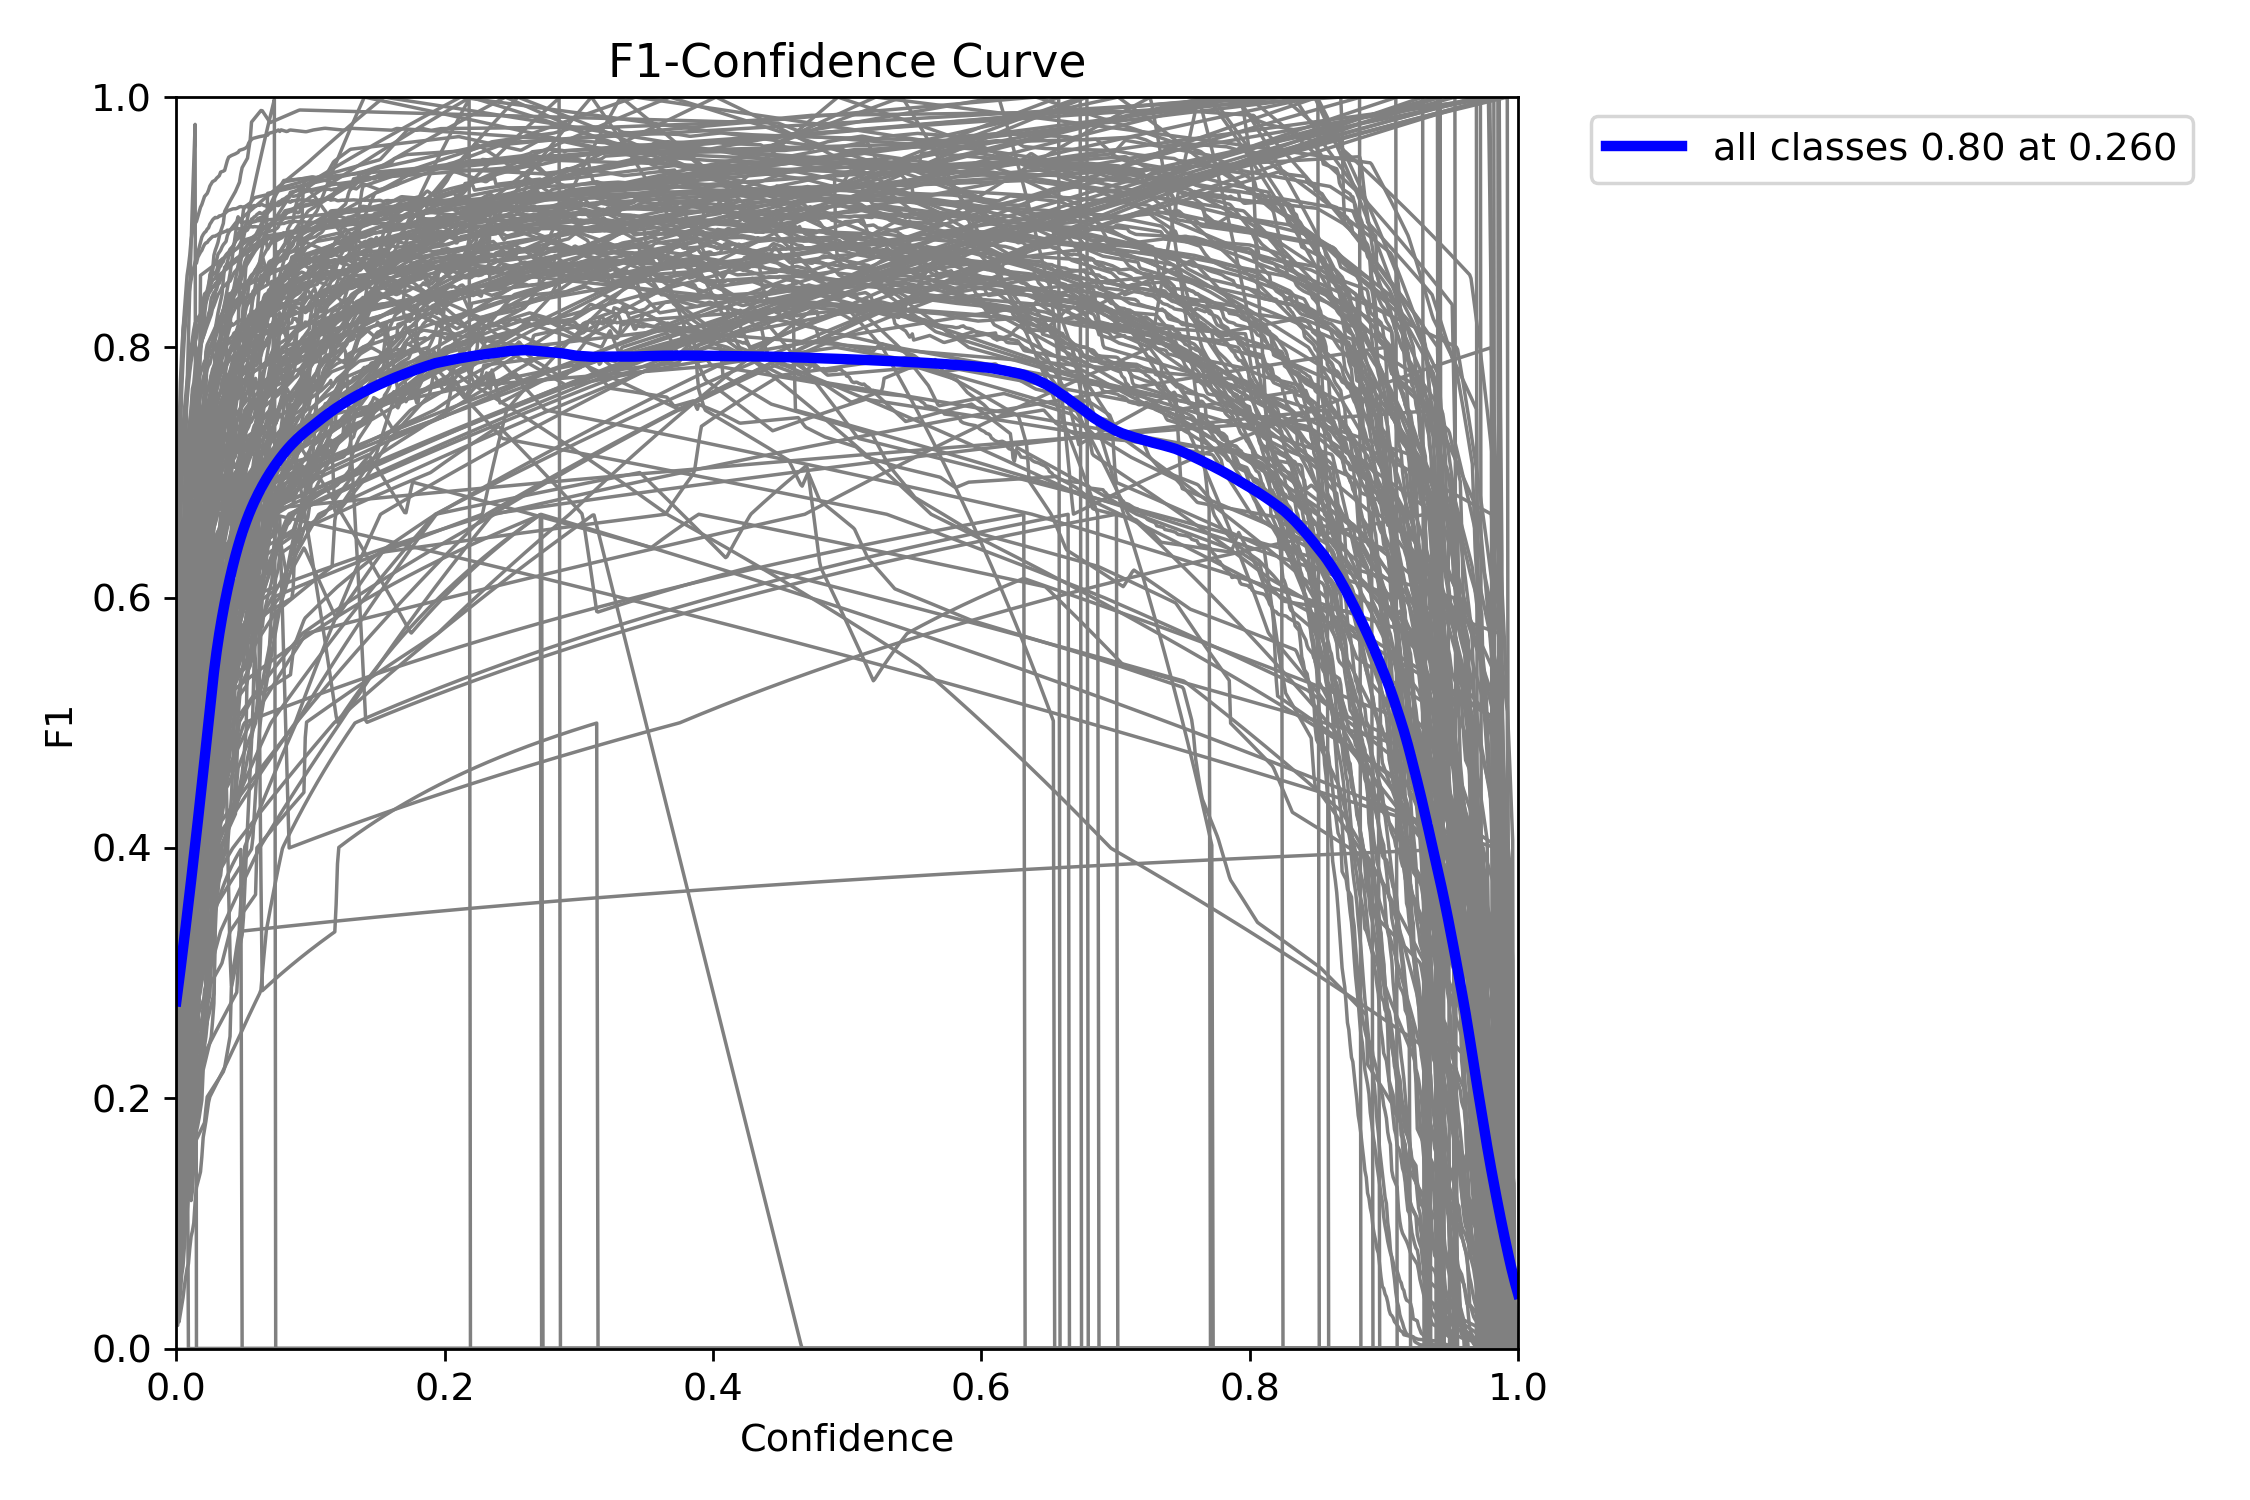
\includegraphics[width=0.4\textwidth]{../figure/tt100k_ex_F1_curve.png}
        }
        \subfloat[YOLOv11s\label{fig:fogtt100k_11s_f1}]{
            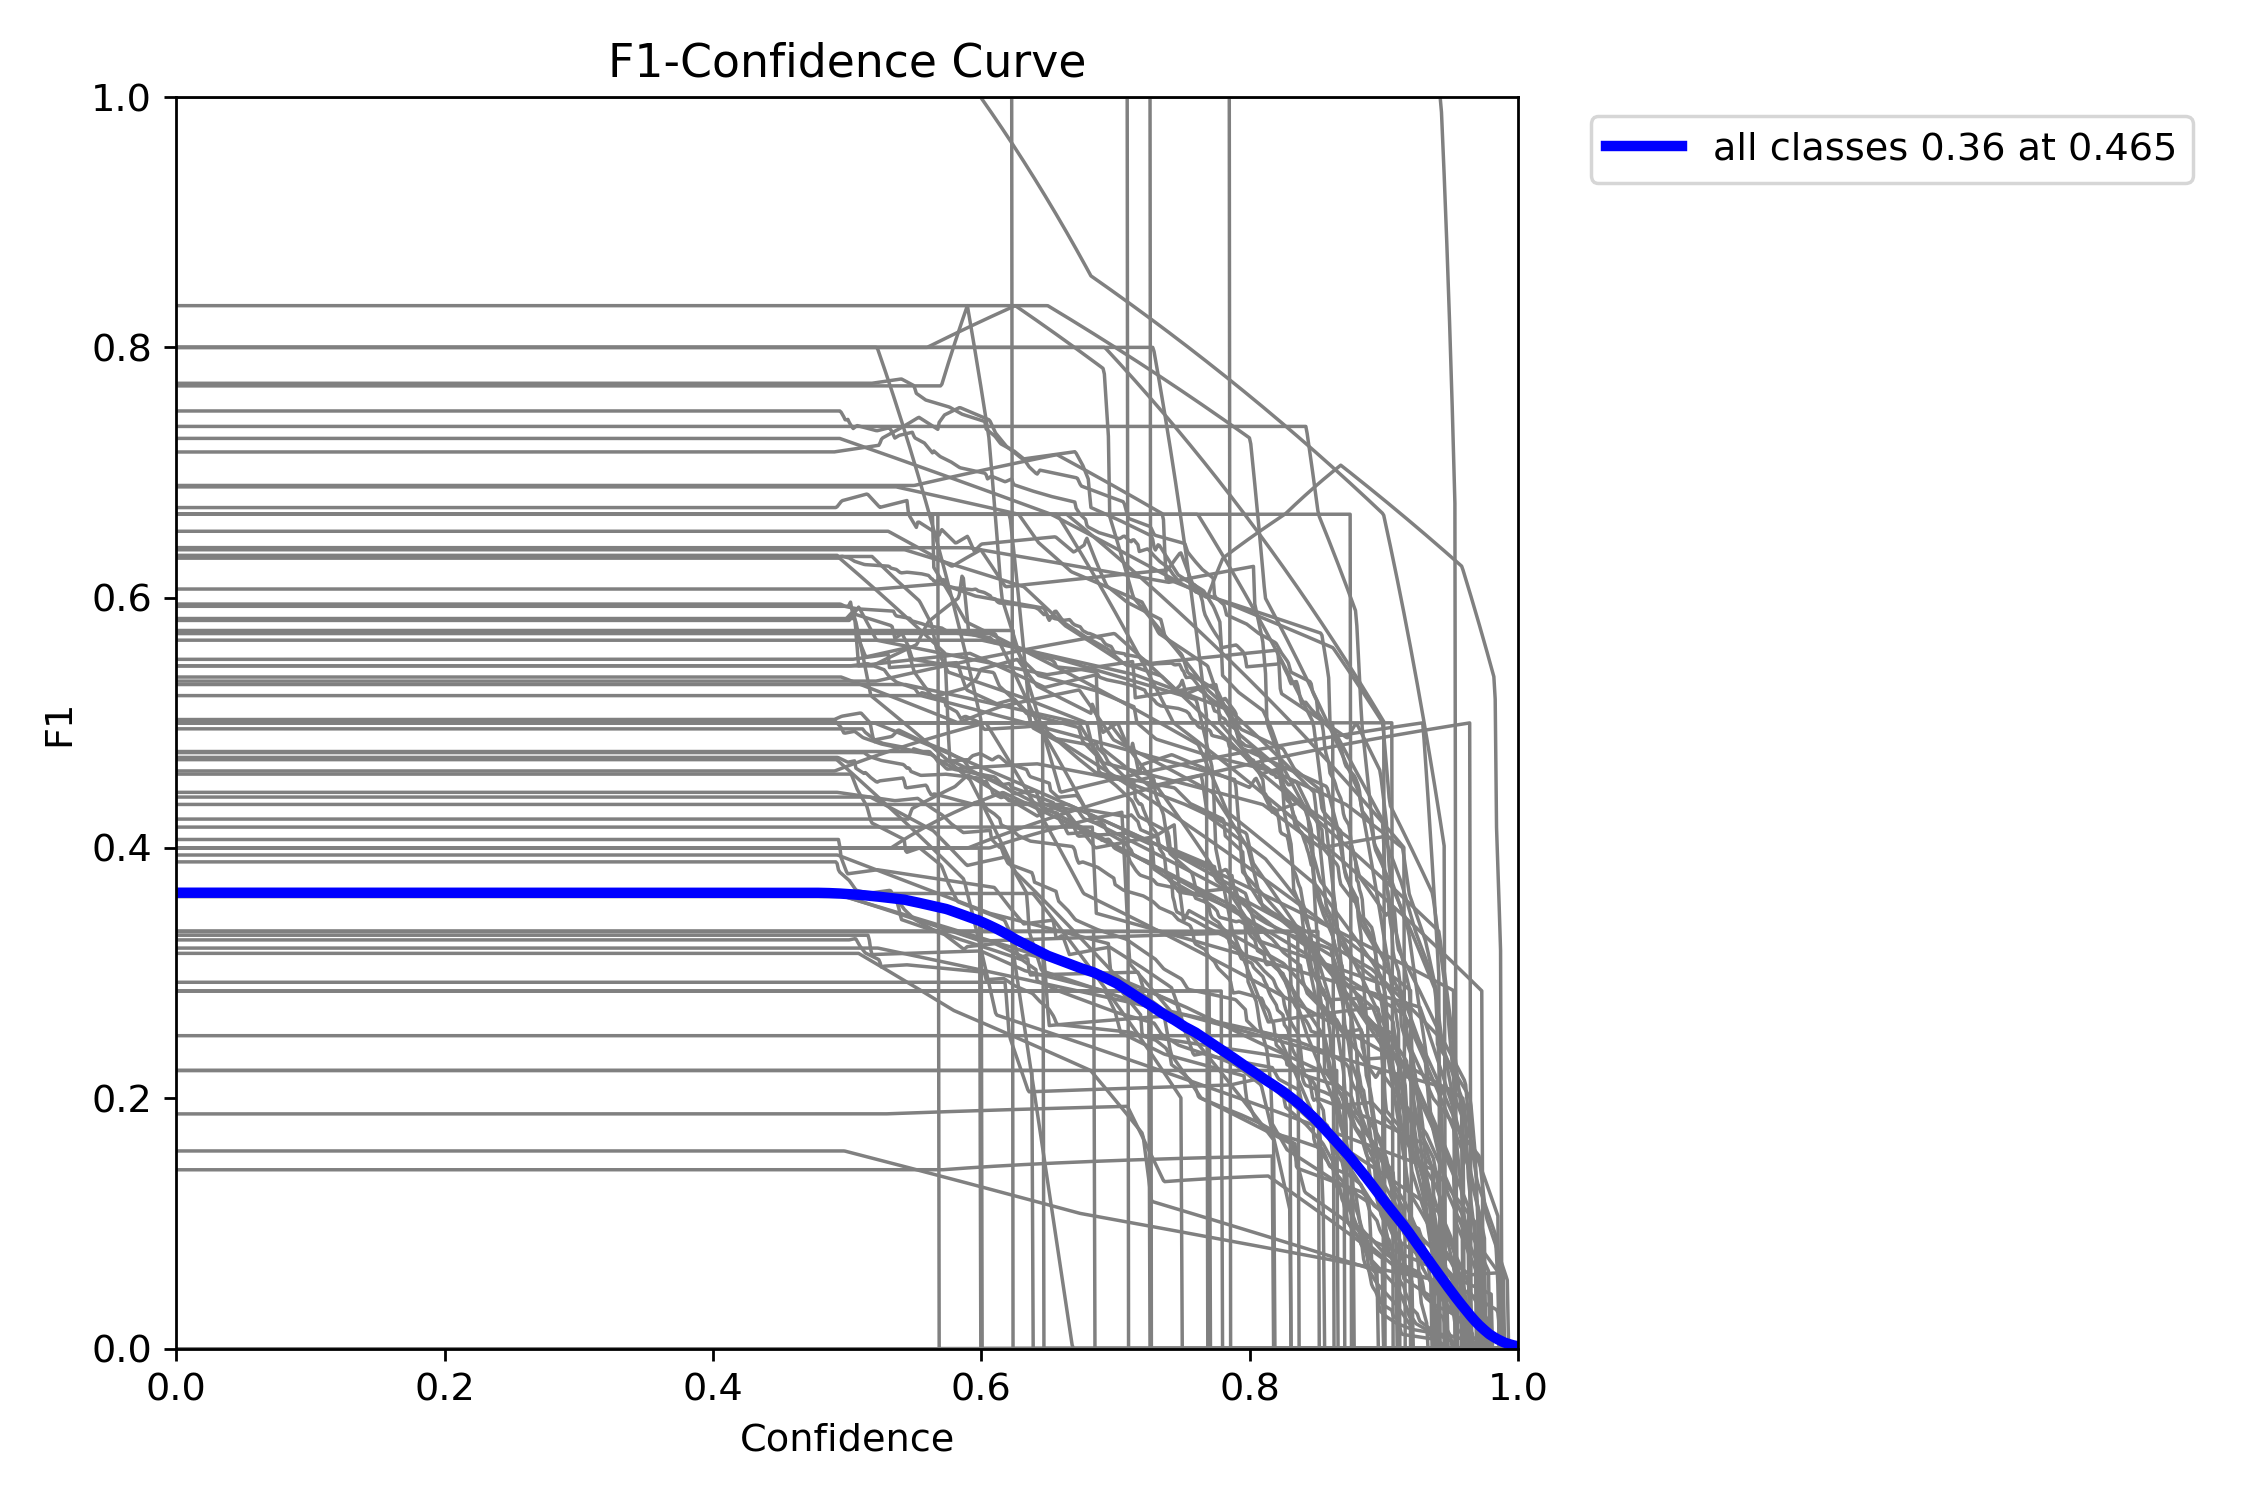
\includegraphics[width=0.4\textwidth]{../figure/fogtt_11_F1_curve.png}
        } \\
        \subfloat[YOLOv10s\label{fig:fogtt100k_10s_f1}]{
            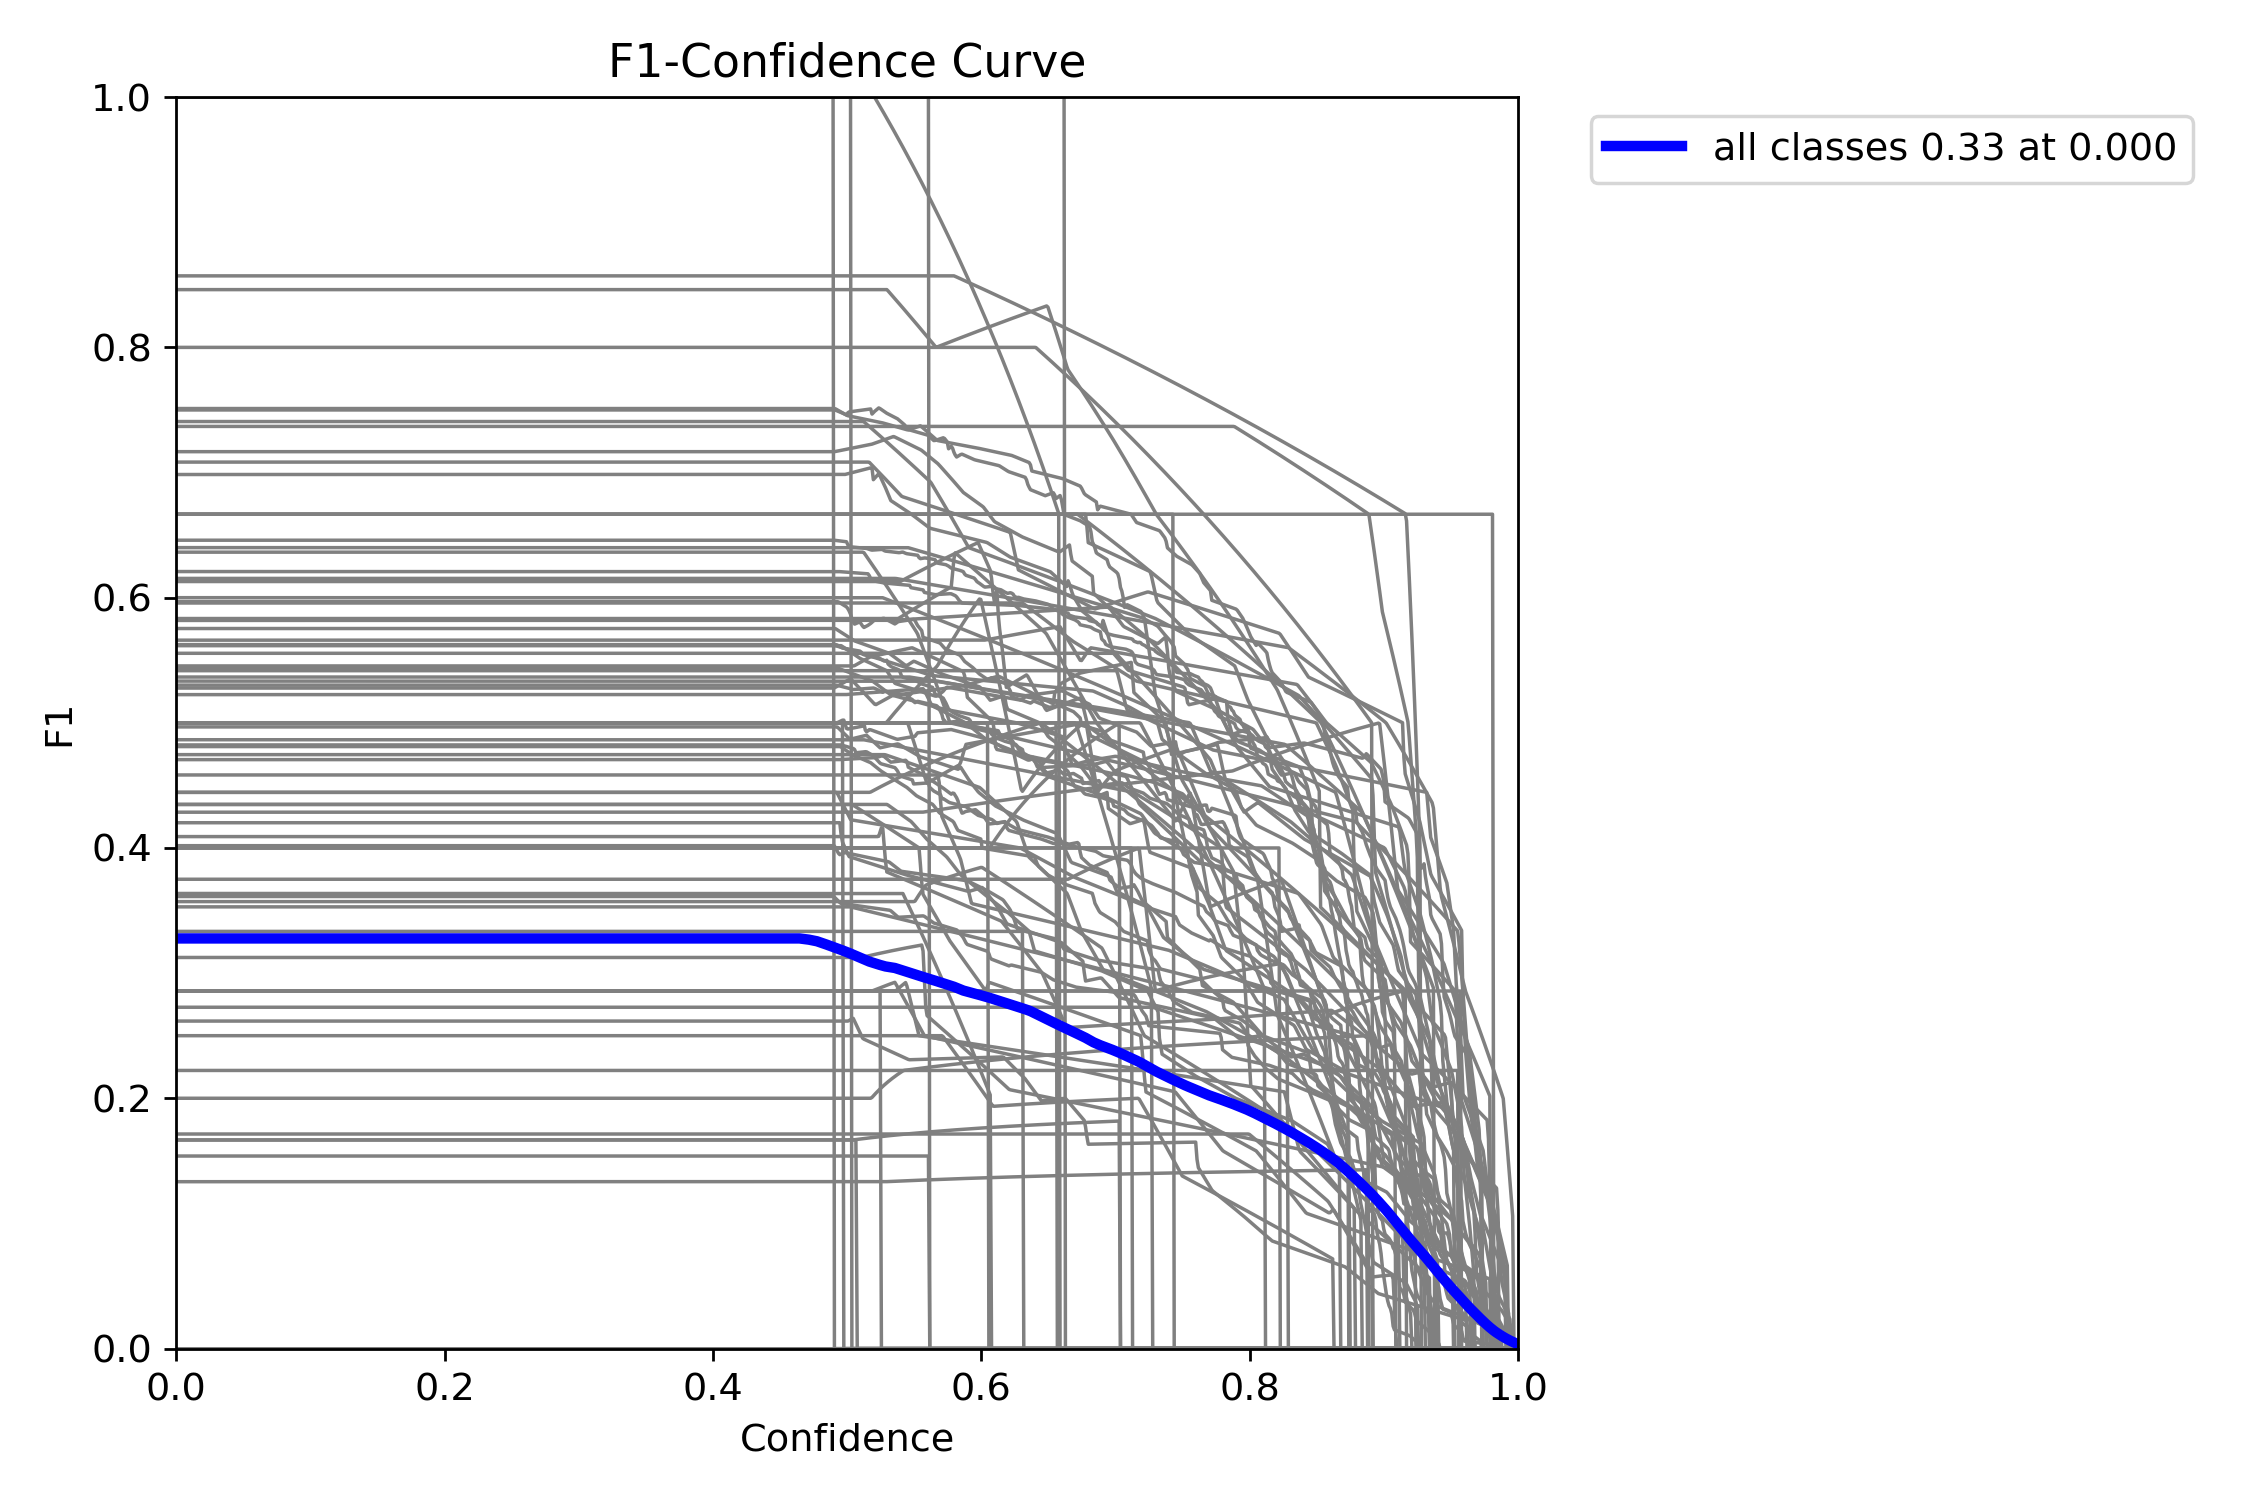
\includegraphics[width=0.4\textwidth]{../figure/fogtt_10_F1_curve.png}
        }
        \subfloat[YOLOv9s\label{fig:fogtt100k_9s_f1}]{
            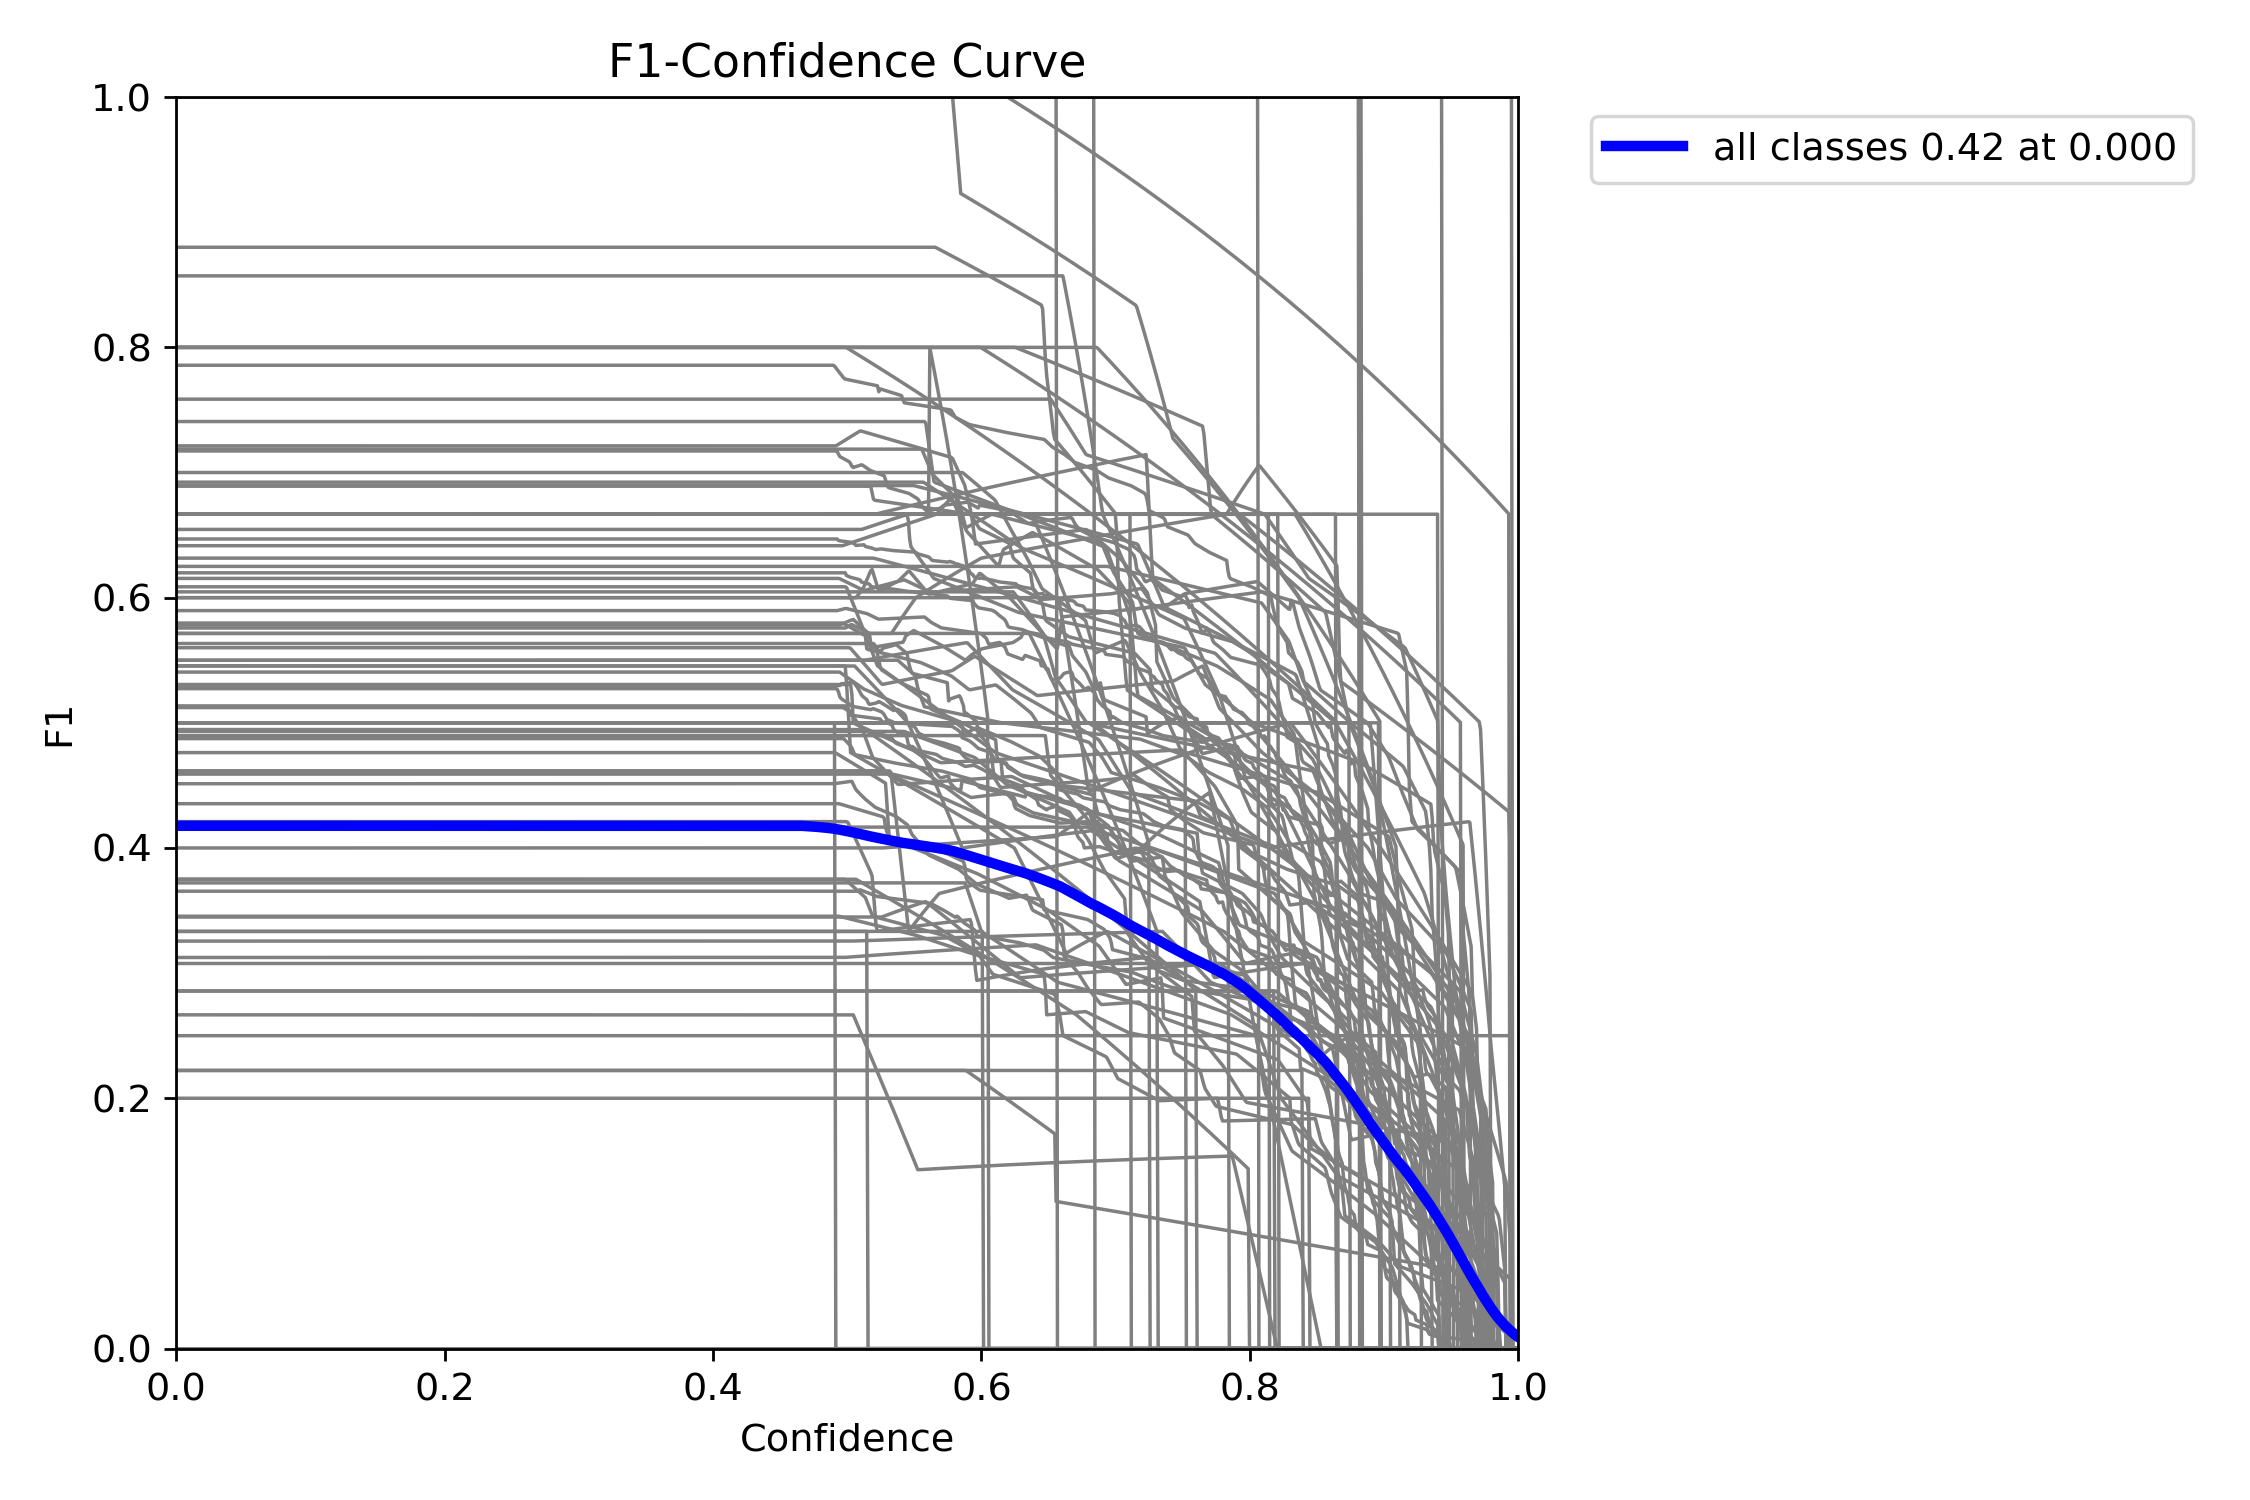
\includegraphics[width=0.4\textwidth]{../figure/fogtt_9_F1_curve.png}
        }
    \captionsetup{font=footnotesize}
    \bicaption{不同的网络模型在 FOG-TT100K 数据集上的F1得分}{F1 scores of different network models on the FOG-TT100K dataset.}
    \label{fig:fogtt100k_f1}
\end{figure}

在精确度(P)方面,YOLOv9s 表现最佳,达到 0.666,our 模型为 0.678,优于 YOLOv11s 的 0.615 和 YOLOv10s 的 0.570,展现出色的精确检测能力。

在召回率(R)方面,our 模型达到 0.321,虽略低于 YOLOv9s 的 0.328,但高于 YOLOv11s 的 0.280 和 YOLOv10s 的 0.249,说明其在目标检测全面性上具有一定优势。

图 \ref{fig:fogtt100k_cmn} 呈现了 YOLOv9s、YOLOv10s、YOLOv11s 以及 our 模型在TT100K数据集针对不同类别目标的预测状况。具体而言,图 \ref{fig:fogtt100k_cmn} 为归一化混淆矩阵的热力图形式,其中颜色深浅与预测概率呈正相关,颜色愈深,意味着预测准确率愈高,相应地,颜色愈浅,则表明预测准确率较低。需要强调的是,热力图对角线上的数据对应着模型成功预测正确标签的情况,而非对角线部分的数据则反映了模型出现标签预测错误的情形。

然而,从直观观察的角度来看,图 \ref{fig:fogtt100k_ex_cmn}、图 \ref{fig:fogtt100k_11s_cmn}、图 \ref{fig:fogtt100k_10s_cmn} 以及图 \ref{fig:fogtt100k_9s_cmn} 均难以清晰地辨识出每一个类别具体的预测数据细节。但深入分析可发现,于图 \ref{fig:fogtt100k_ex_cmn} 所示的 our 模型中,预测错误标签几率超过 0.5 的类别数量为 7 个;在图 \ref{fig:fogtt100k_11s_cmn} 展示的 YOLOv11s 模型里,这一数值同样为 7 个;从图 \ref{fig:fogtt100k_10s_cmn} 可知,在 YOLOv10s 模型中,预测错误标签几率大于 0.5 的类别有 9 个;而依据图 \ref{fig:fogtt100k_9s_cmn},YOLOv9s 模型中预测错误标签几率大于 0.5 的类别数量为 4 个。

综合图 \ref{fig:fogtt100k_cmn} 所揭示的归一化混淆矩阵热力图信息,可以明确地得出结论:在 TT100K 数据集上,YOLOv9s 模型在预测正确类别方面展现出更为卓越的性能,这一结论也得到了表 \ref{tab:compare_studies_tt100k} 中相关数据的有力印证 ——YOLOv9s 的精确度和召回率分别达到了 0.914 和 0.818。尽管 our 模型在预测正确标签的性能上稍逊于 YOLOv9s 模型,但与 YOLOv11s 模型相比,our 模型在预测正确标签方面维持了相近的性能水平,且二者的表现均优于 YOLOv10s 模型。

在 mAP 性能方面,our 模型以 0.555 的 $mAP_{0.5}$ 领先,优于 YOLOv11s 的 0.453、YOLOv10s 的 0.414 以及 YOLOv9s 的 0.501,这表明 our 模型在平衡精确度和召回率方面表现出色,在雾天交通场景目标检测任务中具有很强的竞争力,能够有效提升对各类交通目标的综合检测性能。

图 \ref{fig:fogtt100k_f1} 展示了不同模型的F1得分曲线。YOLOv9s的mAP是最高的(0.906),这与其高F1 AUC一致。 我们模型的mAP为0.893,略低于YOLOv9s,但高于YOLOv11s和YOLOv10s。 这表明,尽管our 模型在平均精度上略低于YOLOv9s,但不同F1分数级别的综合性能与YOLOv9s非常接近。 F1曲线的高性能与我们模型的精度和召回率之间的良好平衡有关。 虽然F1曲线的性能略低于YOLOv9s,但our 模型仍然保持了高检测精度和处理速度,同时降低了计算量,这使得它在无人机的小目标检测任务中具有很高的实际应用价值。

从计算量来看,our 模型的计算量仅为 17.0 GFLOPs,显著低于 YOLOv11s 的 21.8 GFLOPs、YOLOv10s 的 25.4 GFLOPs 和 YOLOv9s 的 27.2 GFLOPs。这使得 our 模型在保持较高检测精度的同时,具备更低的计算复杂度,更有利于在资源受限的设备(如无人机)上进行实时目标检测,可有效提高无人机在复杂雾天场景下对交通目标的检测效率和实用性,为其在实际交通管理、智能驾驶辅助等领域的应用提供了有力支持。尽管参数量稍高(11.4 MB),但综合考虑其在精度和计算效率方面的优势,这种参数量的增加是合理且值得的,our 模型成功实现了在雾天交通场景目标检测任务中精度与效率的良好平衡。


\begin{table}[htbp]
    \centering
    \captionsetup{font=footnotesize}
    \bicaption{在 FOG-VisDrone 数据集上的对比实验结果}{Symbol cross-reference table}
    \label{tab:compare_studies_fogvd}
    \begin{tabular}{p{0.13\textwidth}p{0.12\textwidth}p{0.13\textwidth}p{0.19\textwidth}p{0.09\textwidth}p{0.07\textwidth}p{0.07\textwidth}}
        \toprule
        模型         & 图像大小 & 参数量 MB & 计算量 GFLOPs  & $mAP_{0.5}$     & P     & R     \\ %& FPS \\ 
        \midrule
        YOLOv11s     & 400     & 9.4   & 21.3          & 0.339           & 0.631  & 0.049 \\%& 82.6 \\
        YOLOv10s     & 400     & 8.0   & 24.5          & 0.364           & 0.674  & 0.054 \\%& 78.1 \\
        YOLOv9s      & 400     & 7.2   & 26.7          & 0.348           & 0.642  & 0.055 \\%& 62.1 \\
        \textbf{our} & 400     & 11.4  & \textbf{15.4} & \textbf{0.397}  & 0.721  & 0.074 \\%& 68.5 \\
        \bottomrule
    \end{tabular}
\end{table}

\begin{figure}[htbp]
    \centering
        \subfloat[CGF-YOLO\label{fig:fogvd_ex_cmn}]{
            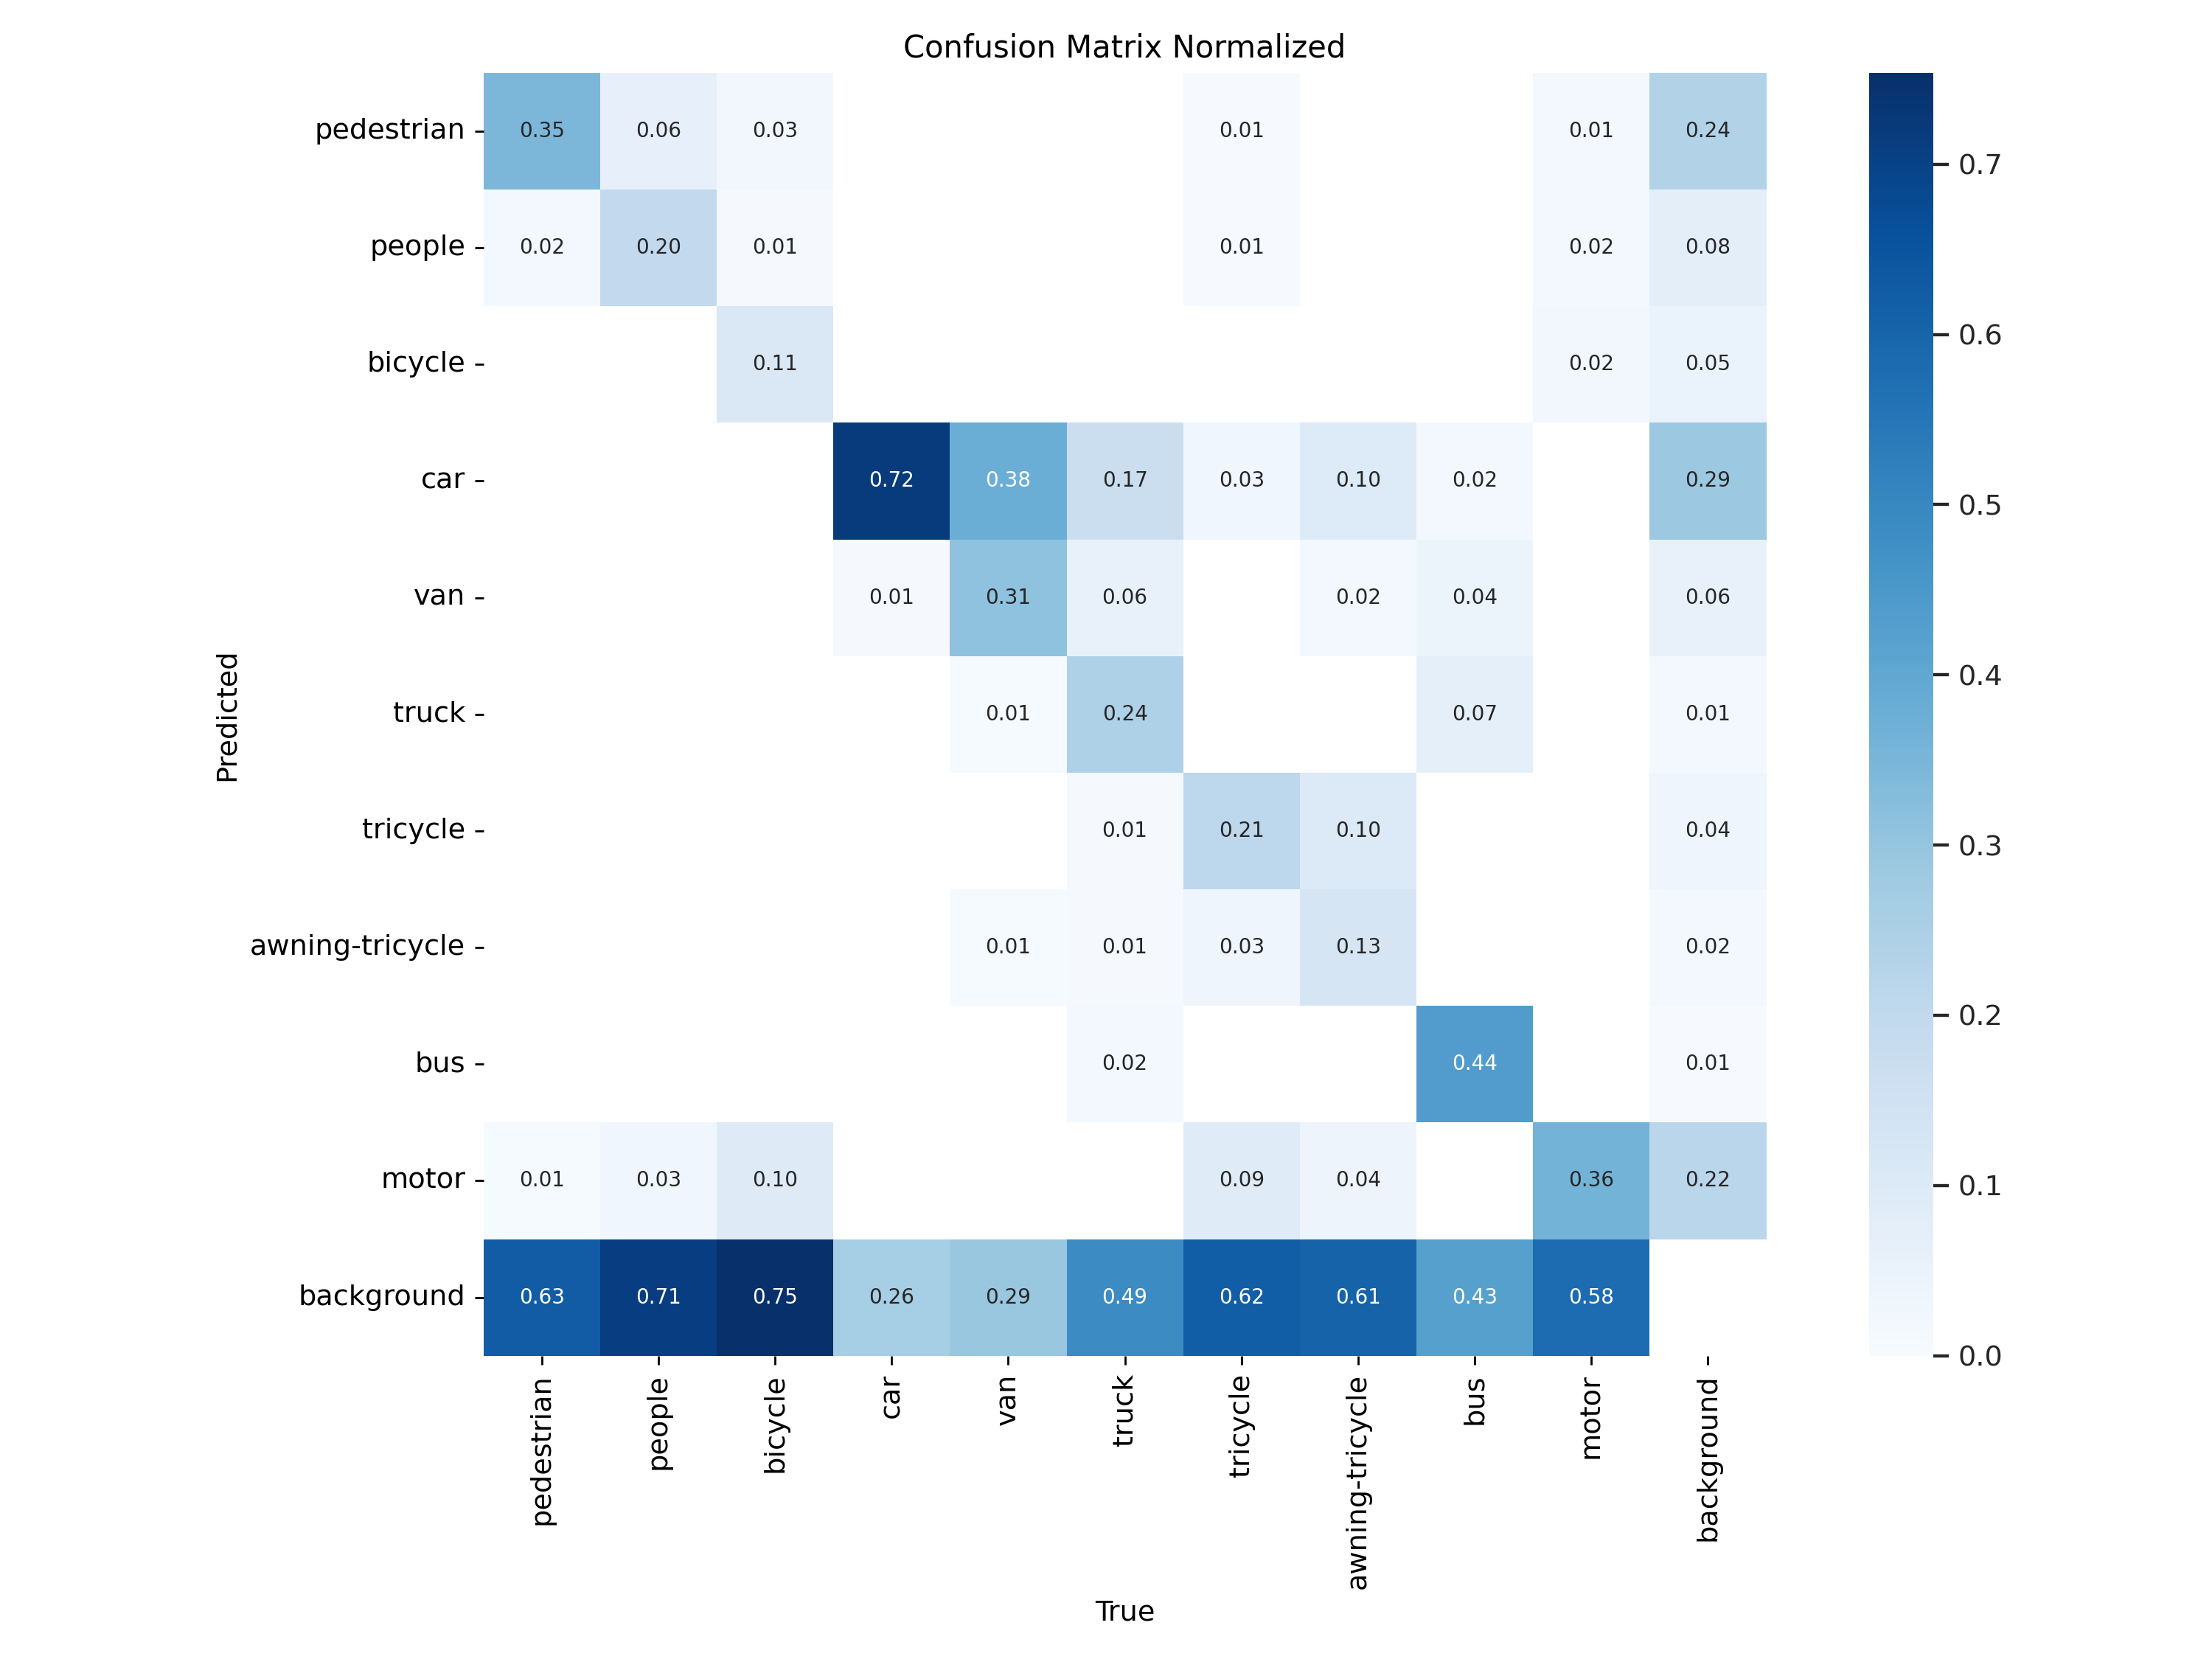
\includegraphics[width=0.4\textwidth]{../figure/vd_ex_confusion_matrix_normalized.png}
        }
        \subfloat[YOLOv11s\label{fig:fogvd_11s_cmn}]{
            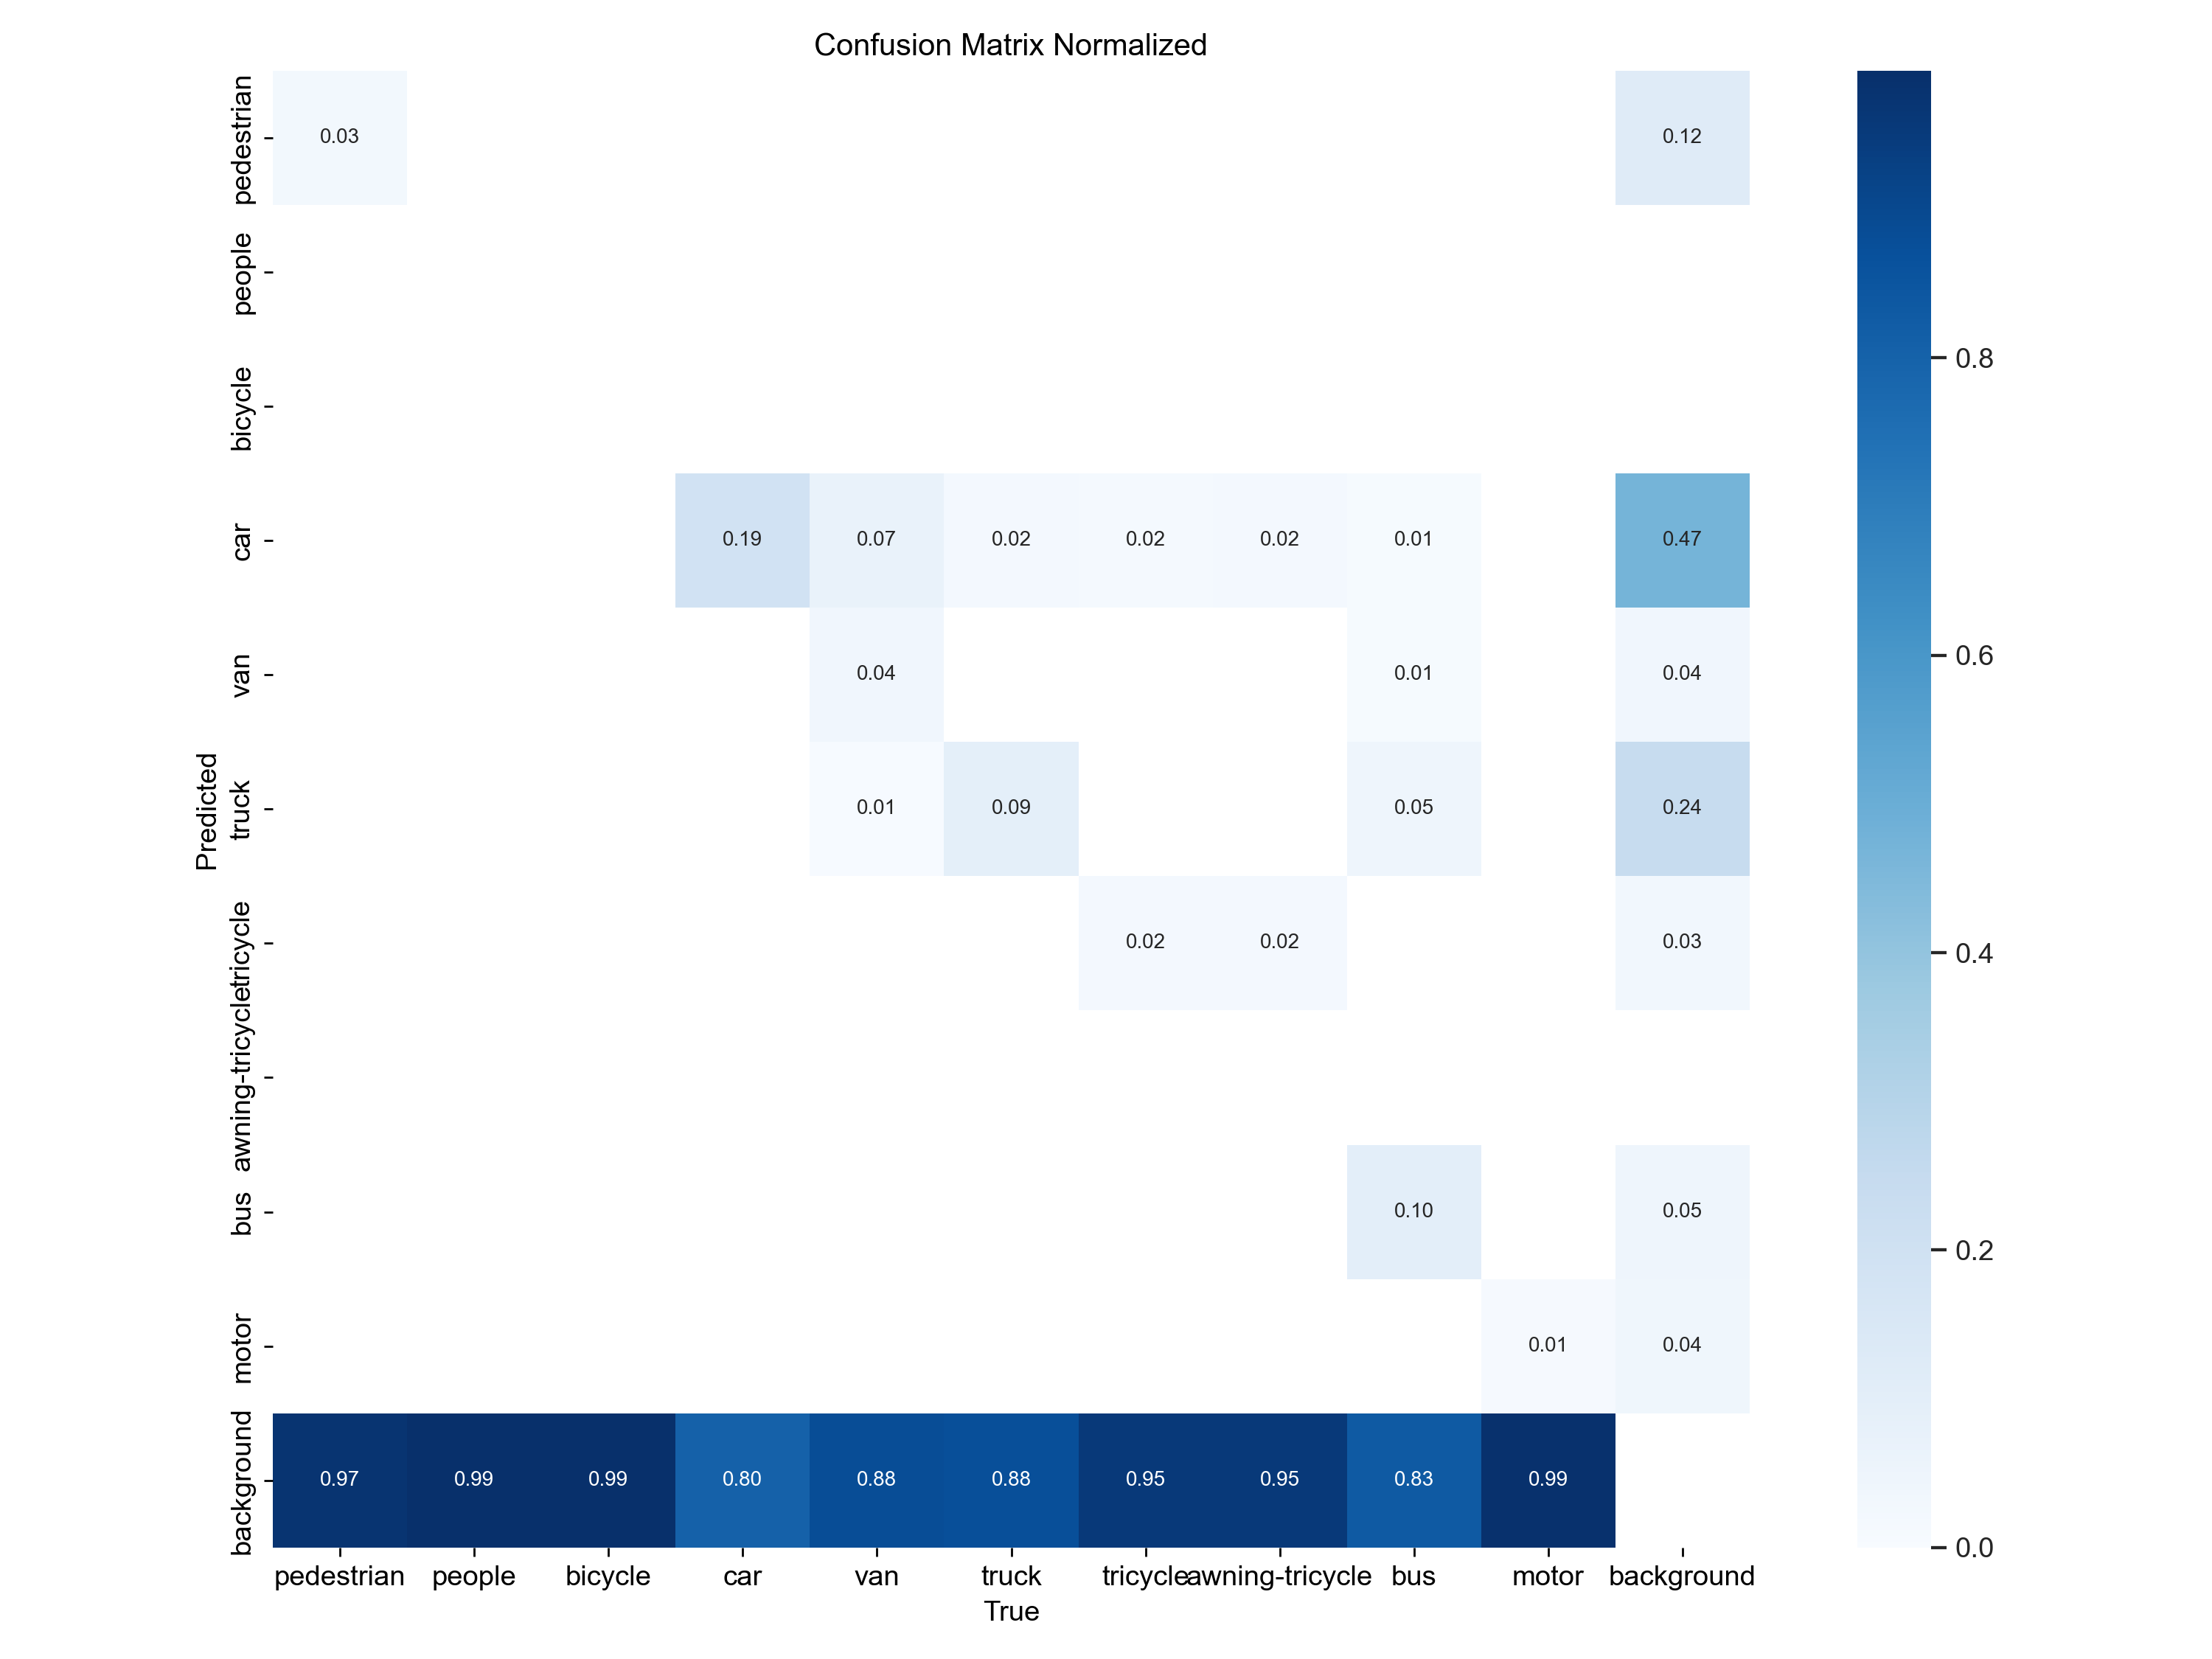
\includegraphics[width=0.4\textwidth]{../figure/fogvd_v11s_confusion_matrix_normalized.png}
        } \\
        \subfloat[YOLOv10s\label{fig:fogvd_10s_cmn}]{
            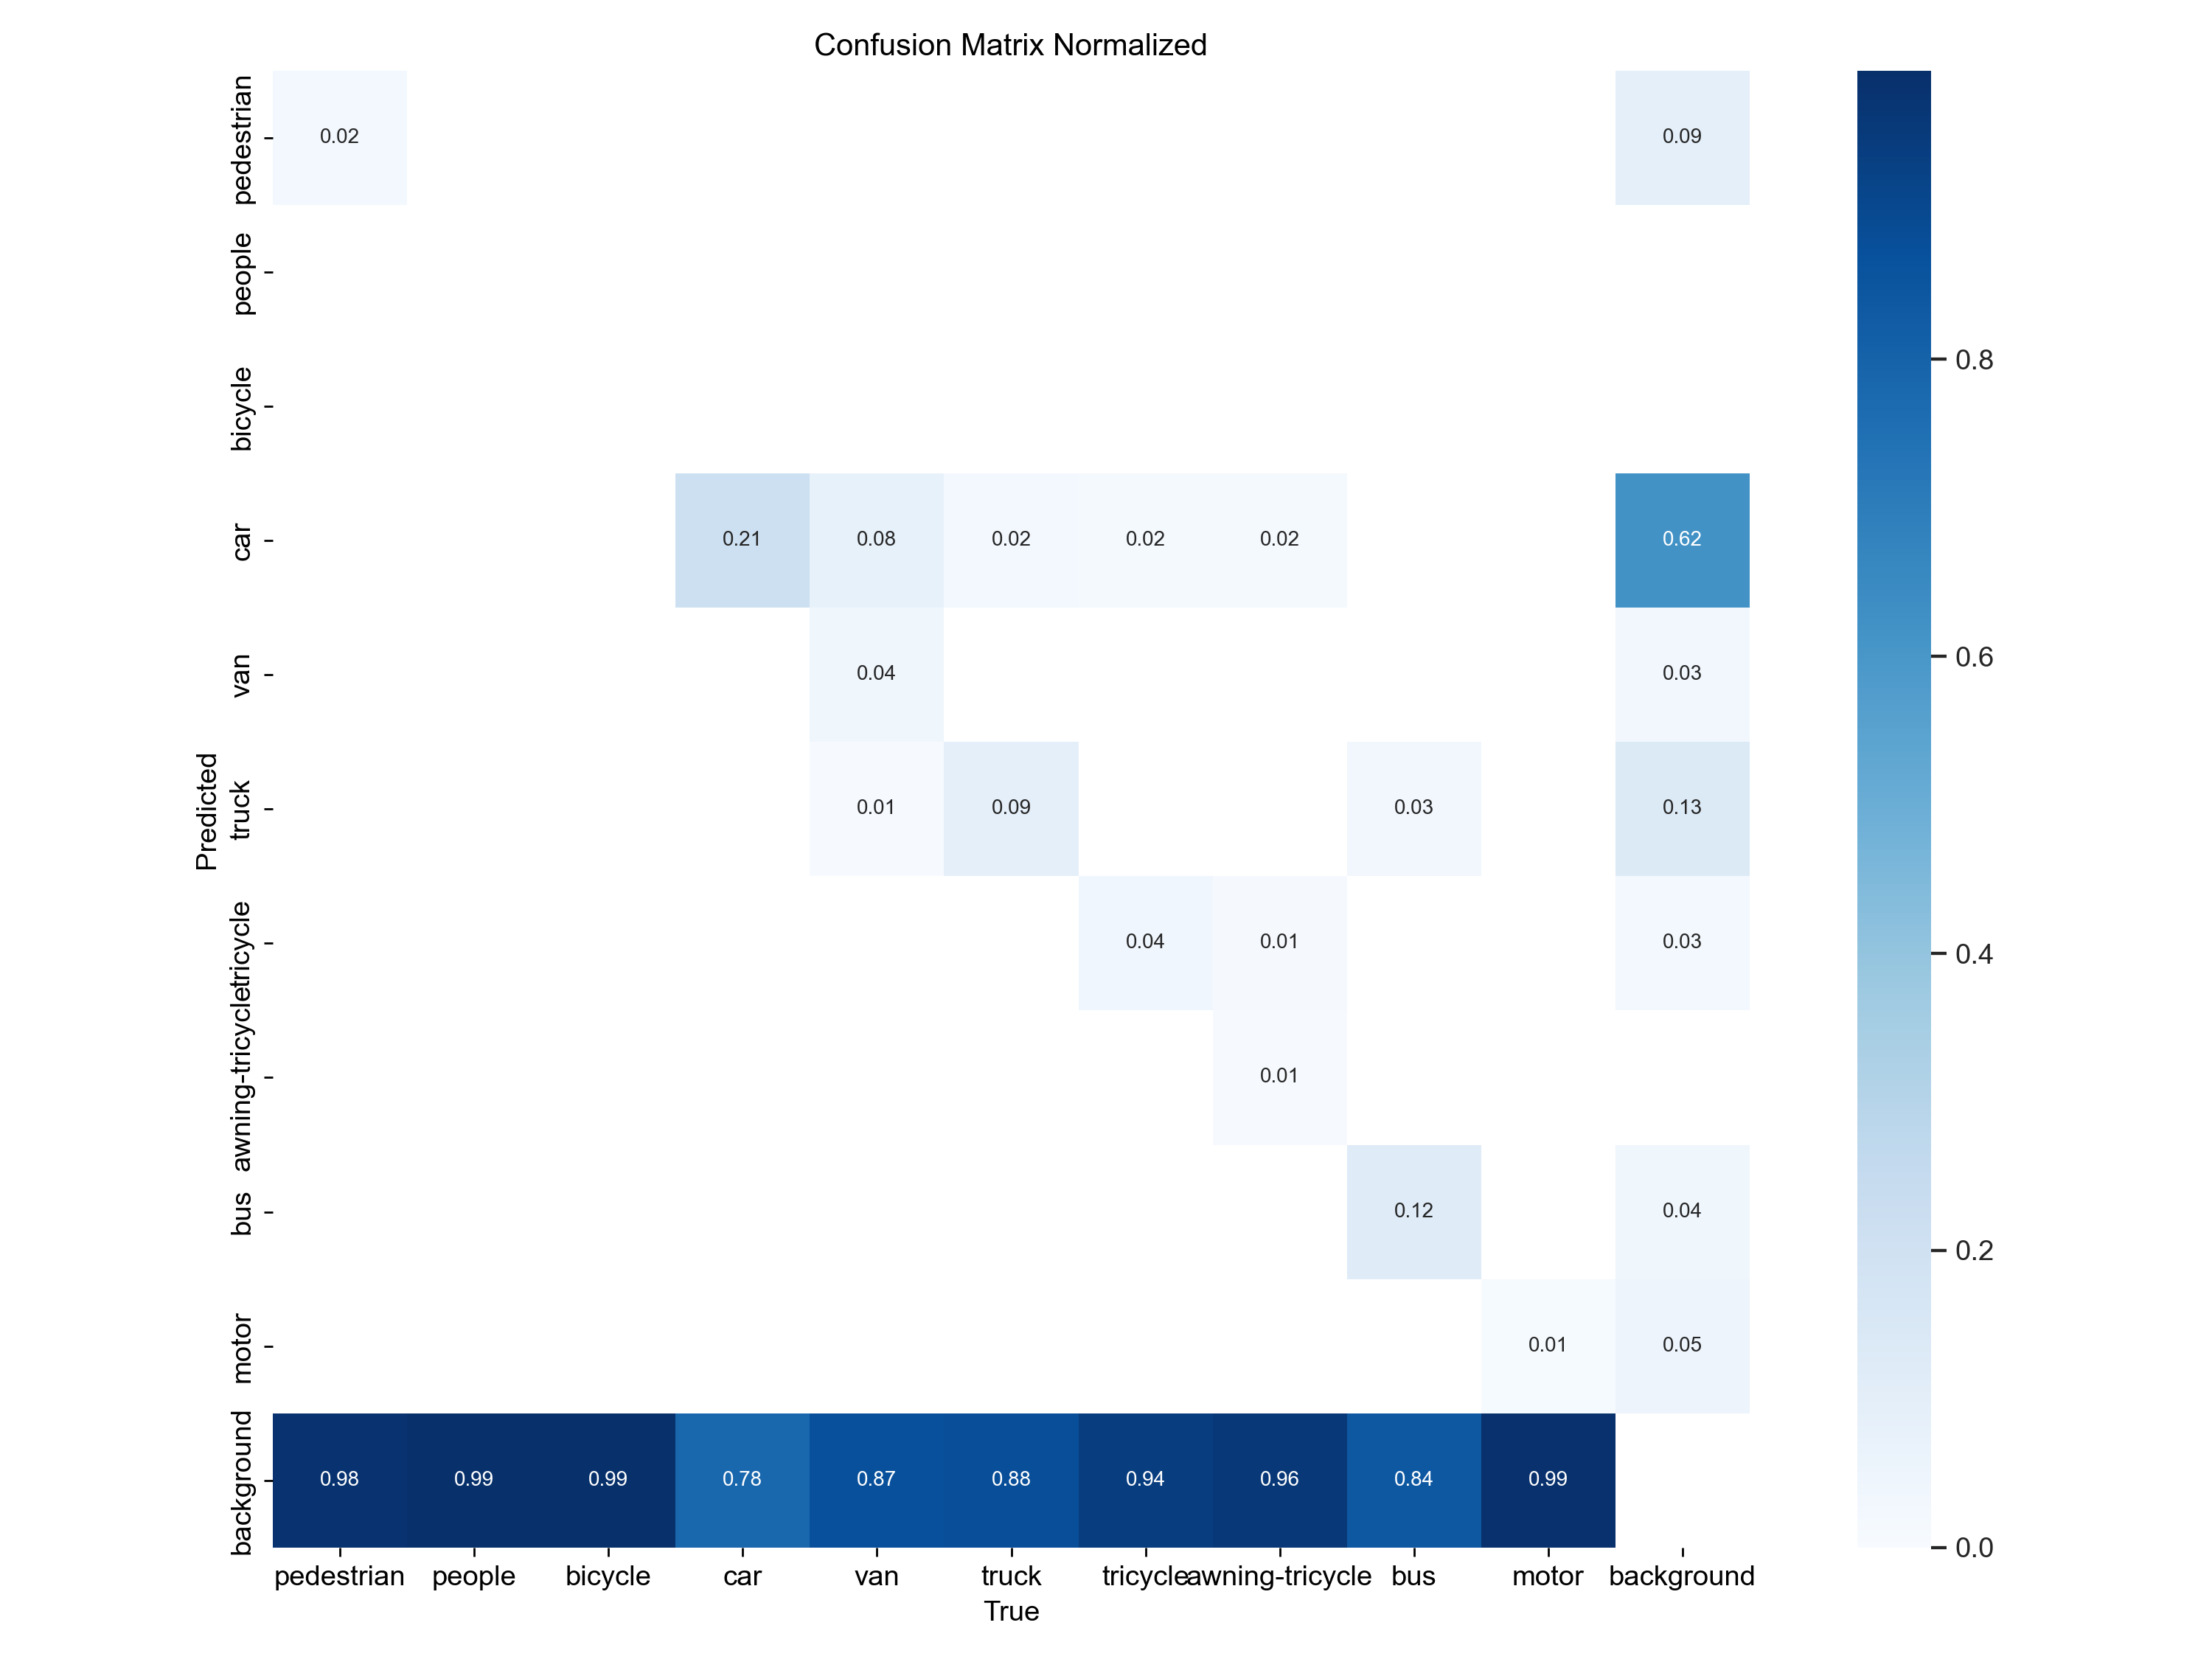
\includegraphics[width=0.4\textwidth]{../figure/fogvd_v10s_confusion_matrix_normalized.png}
        }
        \subfloat[YOLOv9s\label{fig:fogvd_9s_cmn}]{
            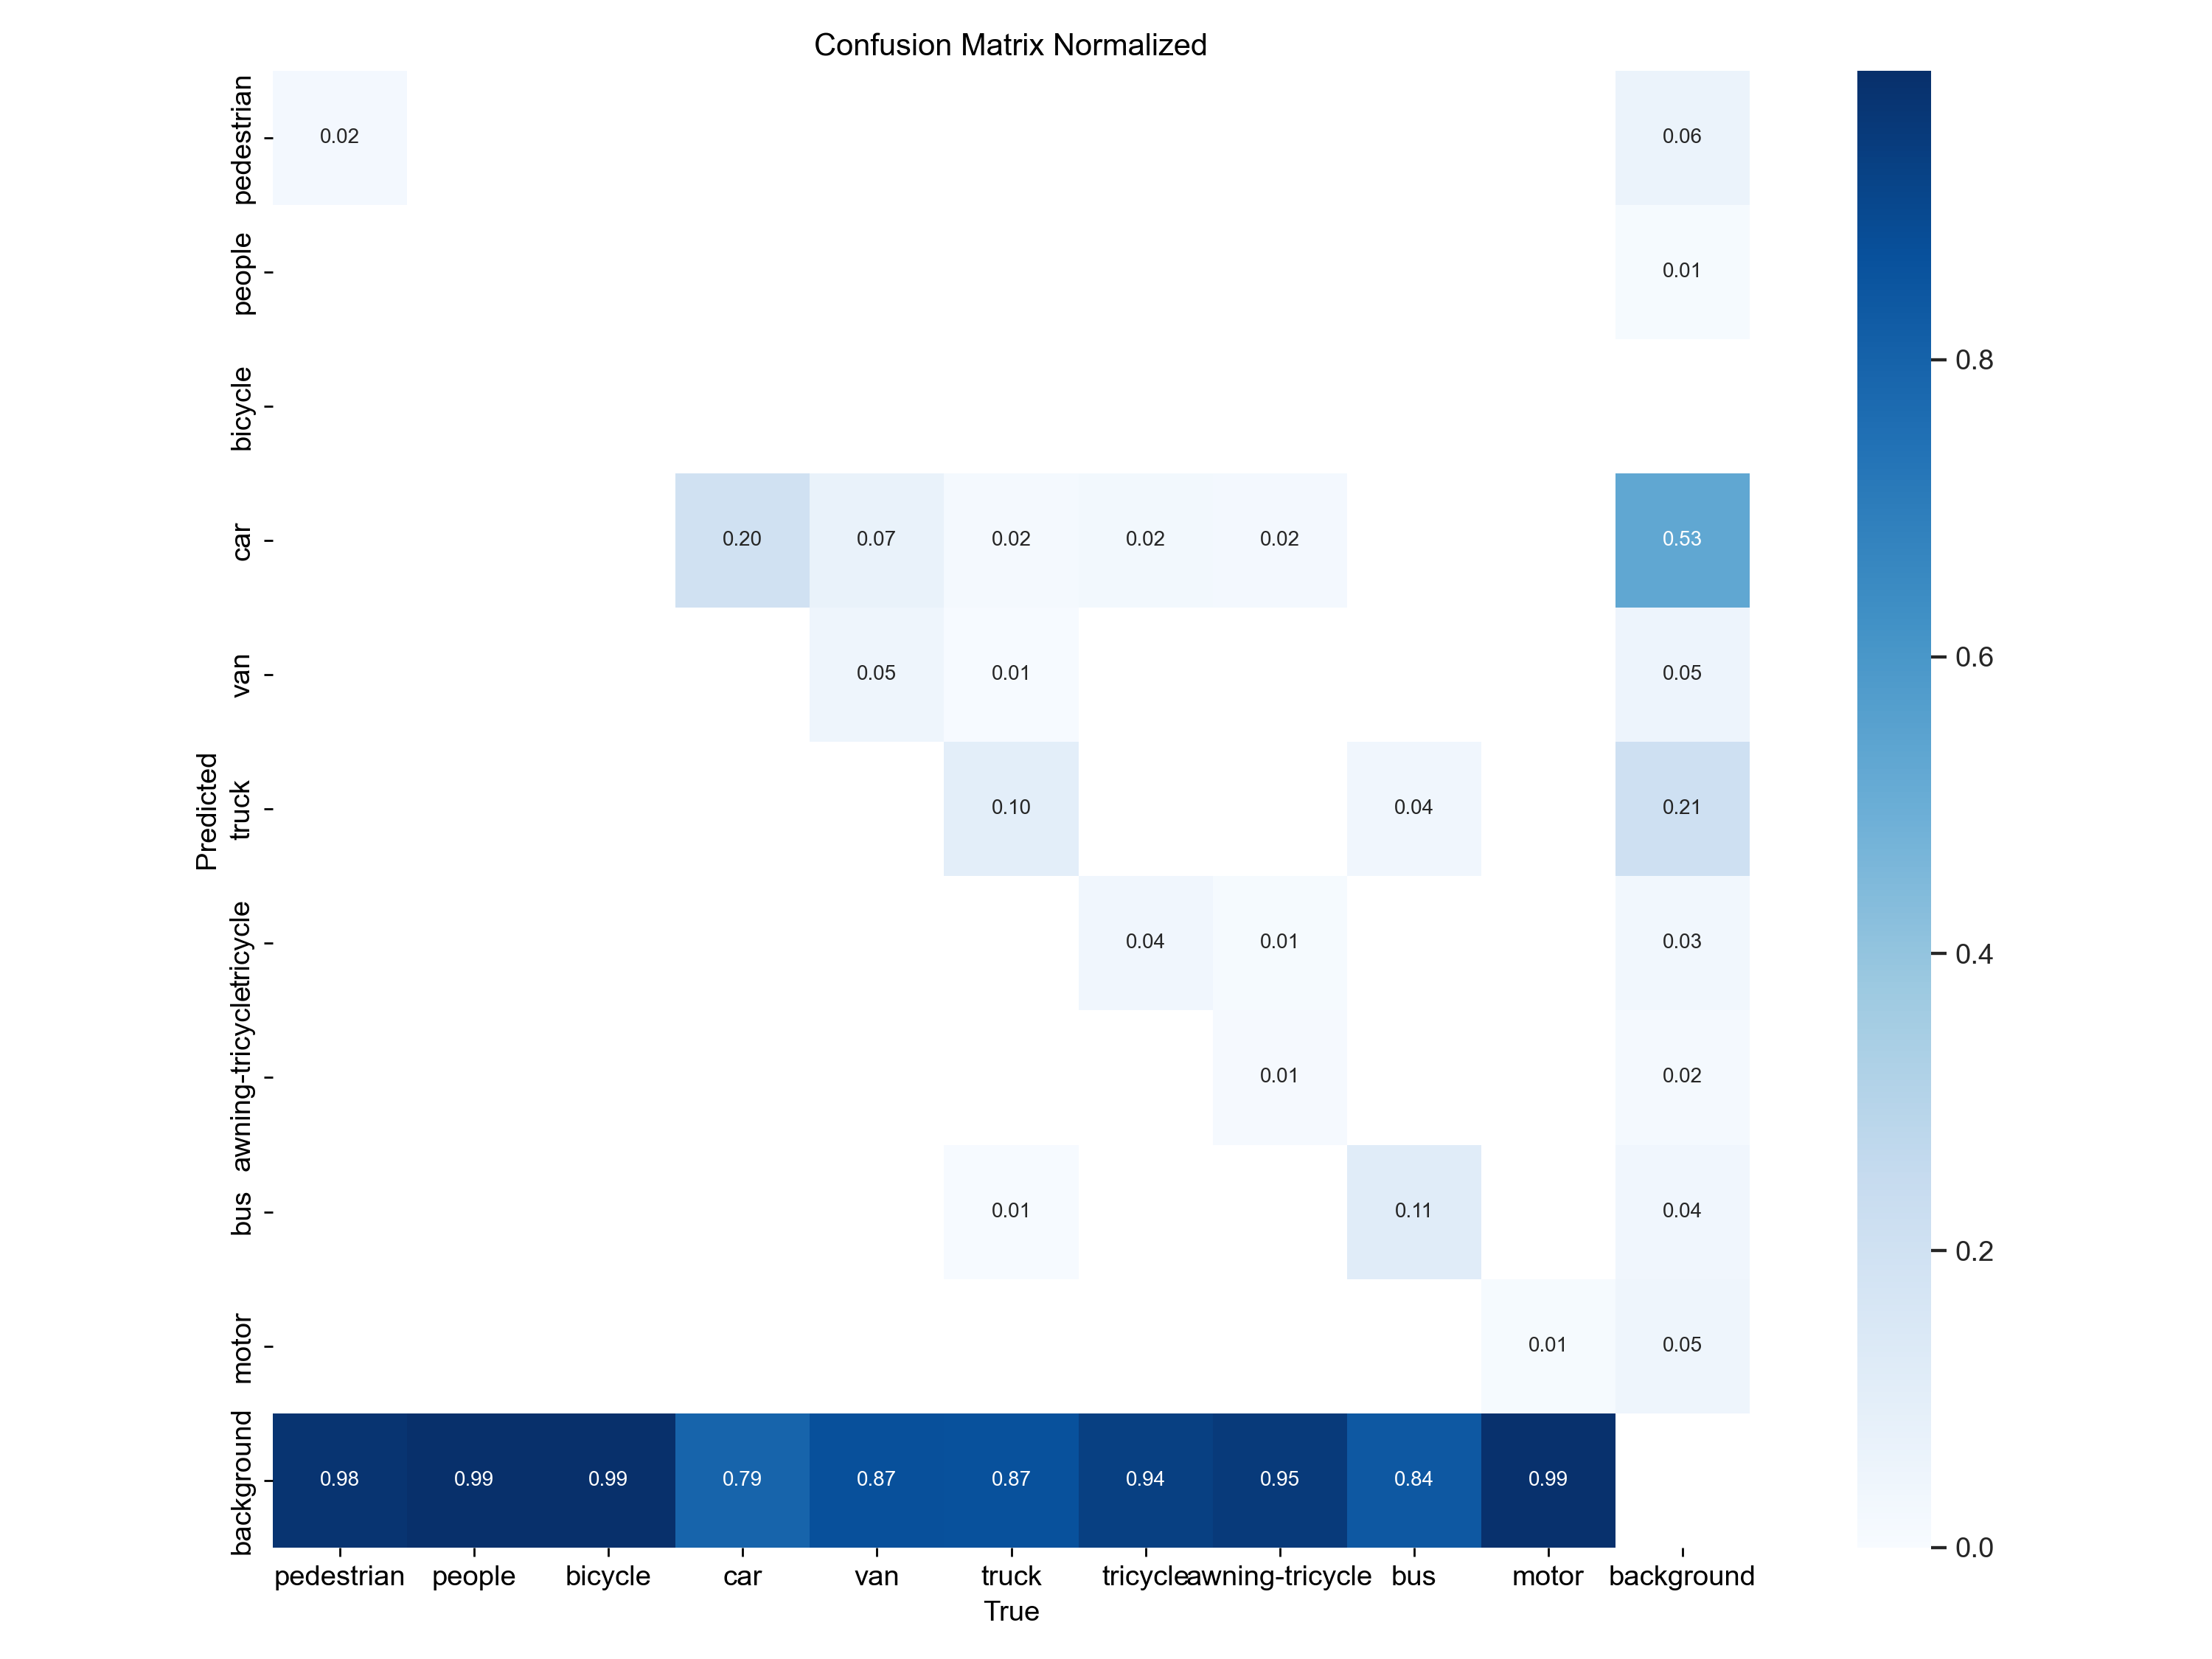
\includegraphics[width=0.4\textwidth]{../figure/fogvd_v9s_confusion_matrix_normalized.png}
        }
    \captionsetup{font=footnotesize}
    \bicaption{不同的网络模型在 FOG-VisDrone 数据集上的归一化混淆矩阵}{The normalized confusion matrix of different network models on the FOG-VisDrone dataset.}
    \label{fig:fogvd_cmn}
\end{figure}

\begin{figure}[htbp]
    \centering
    \subfloat[CGF-YOLO\label{fig:fogvd_ex_f1}]{
        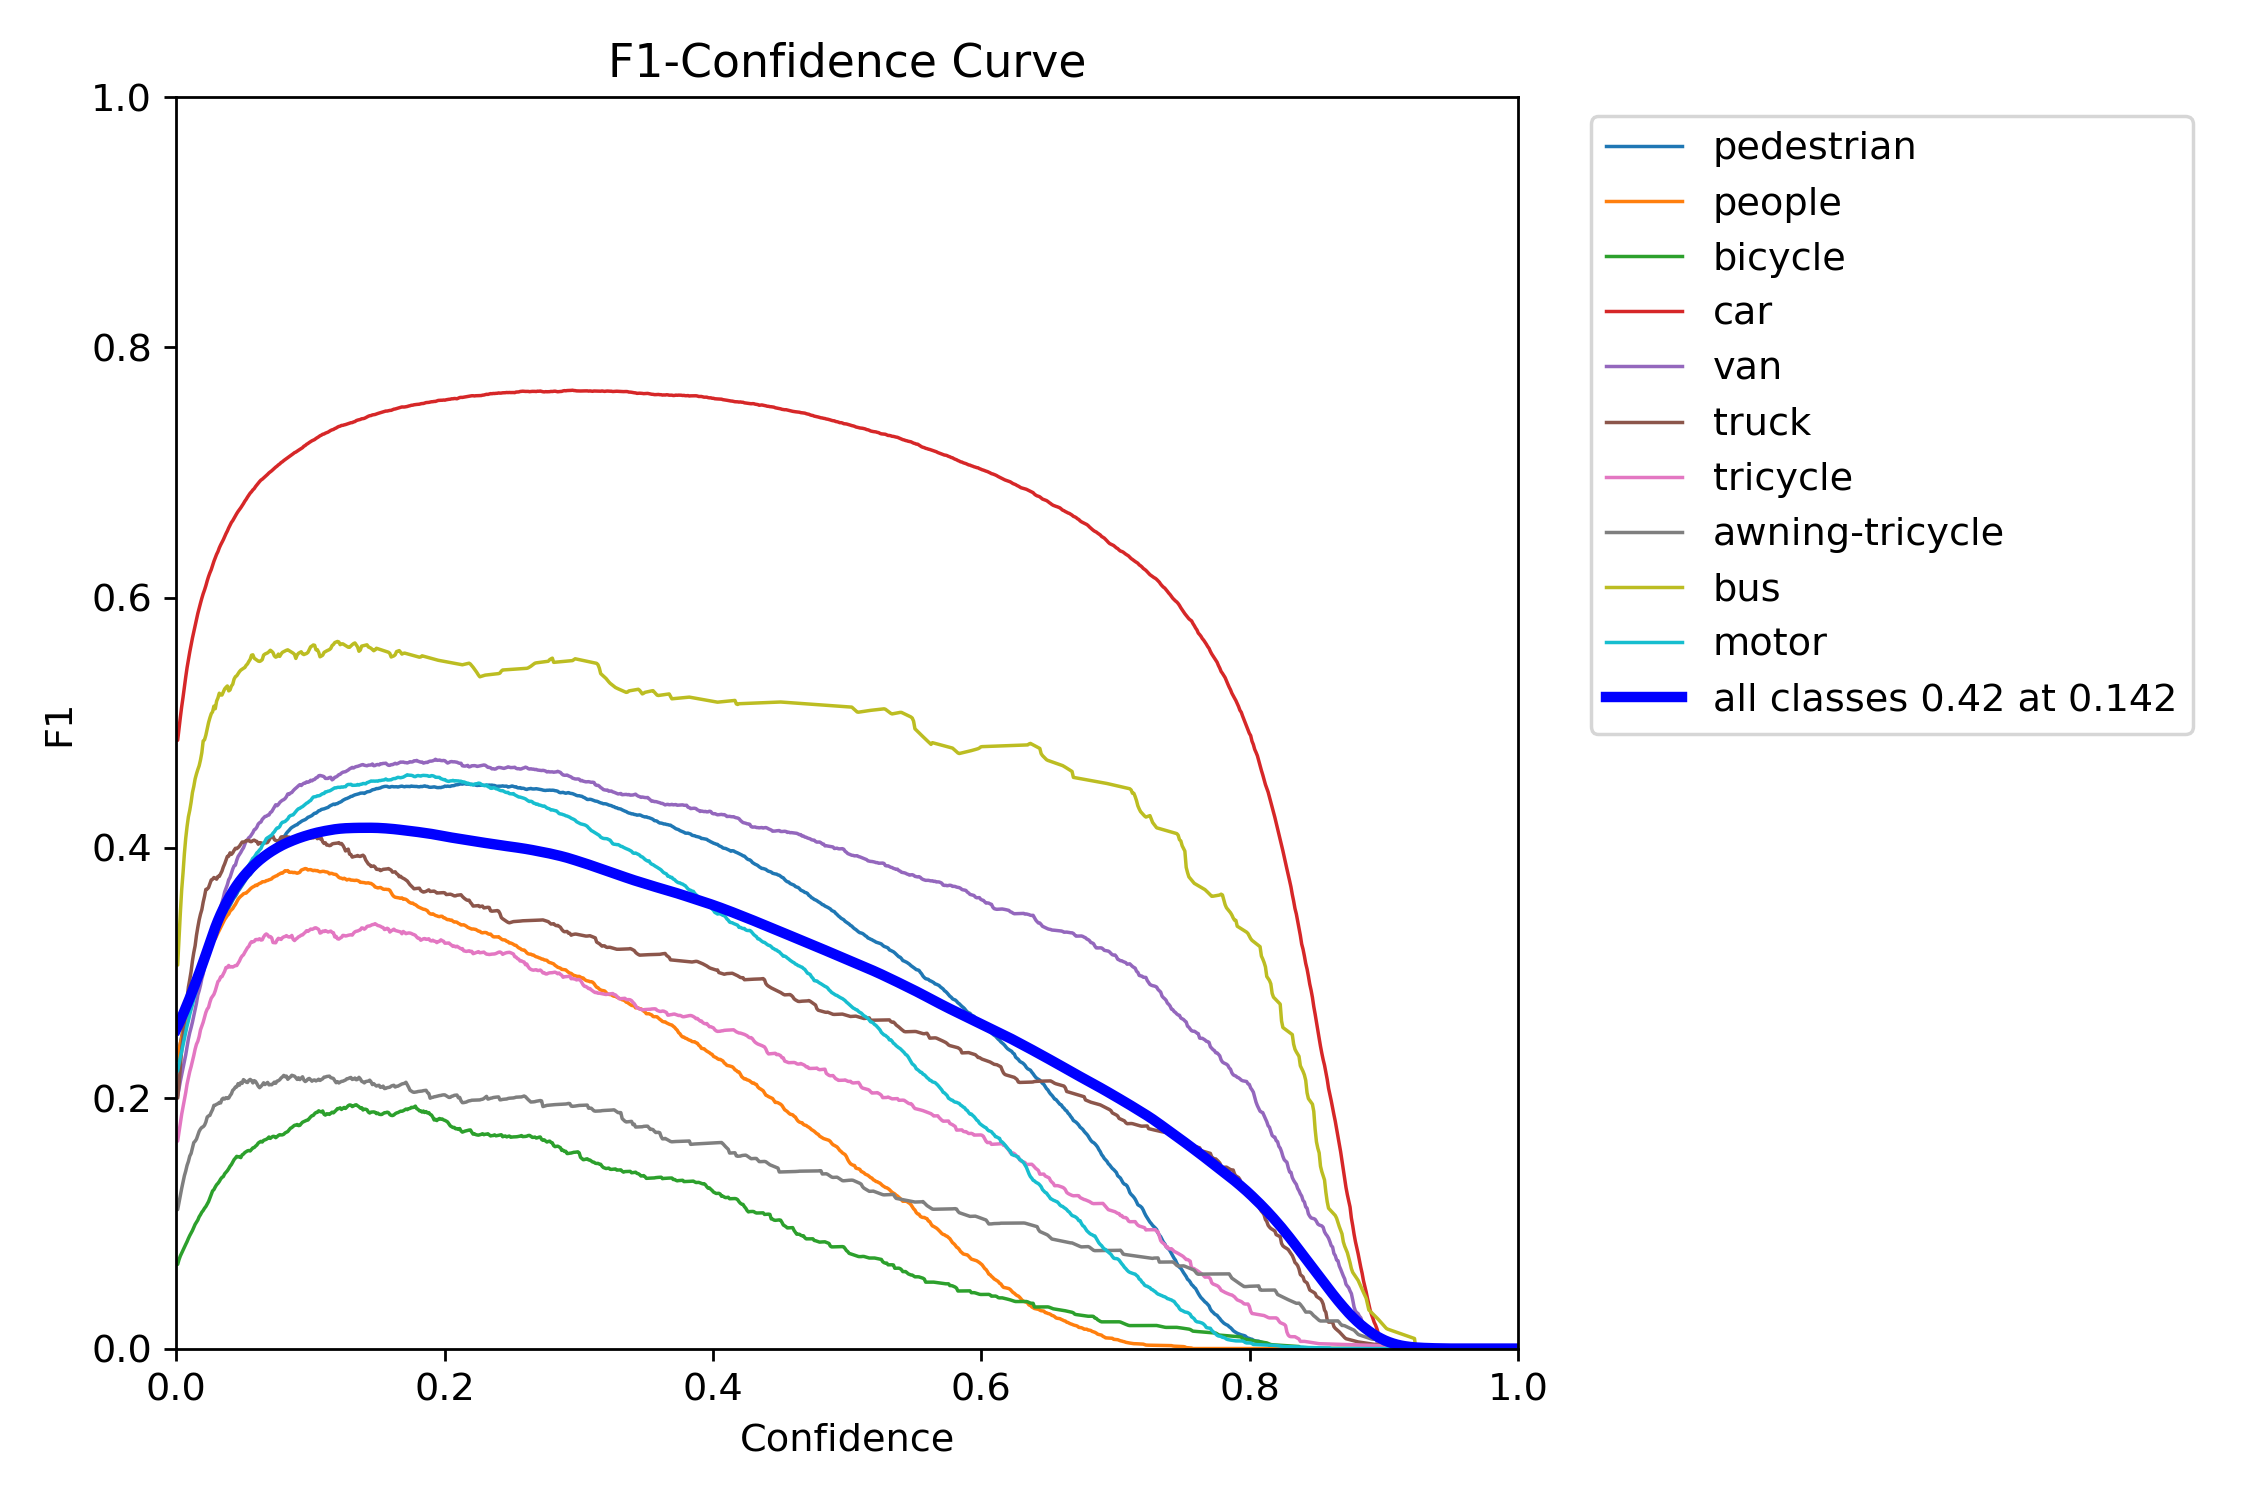
\includegraphics[width=0.4\textwidth]{../figure/vd_ex_F1_curve.png}
    }
    \subfloat[YOLOv11s\label{fig:fogvd_11s_f1}]{
        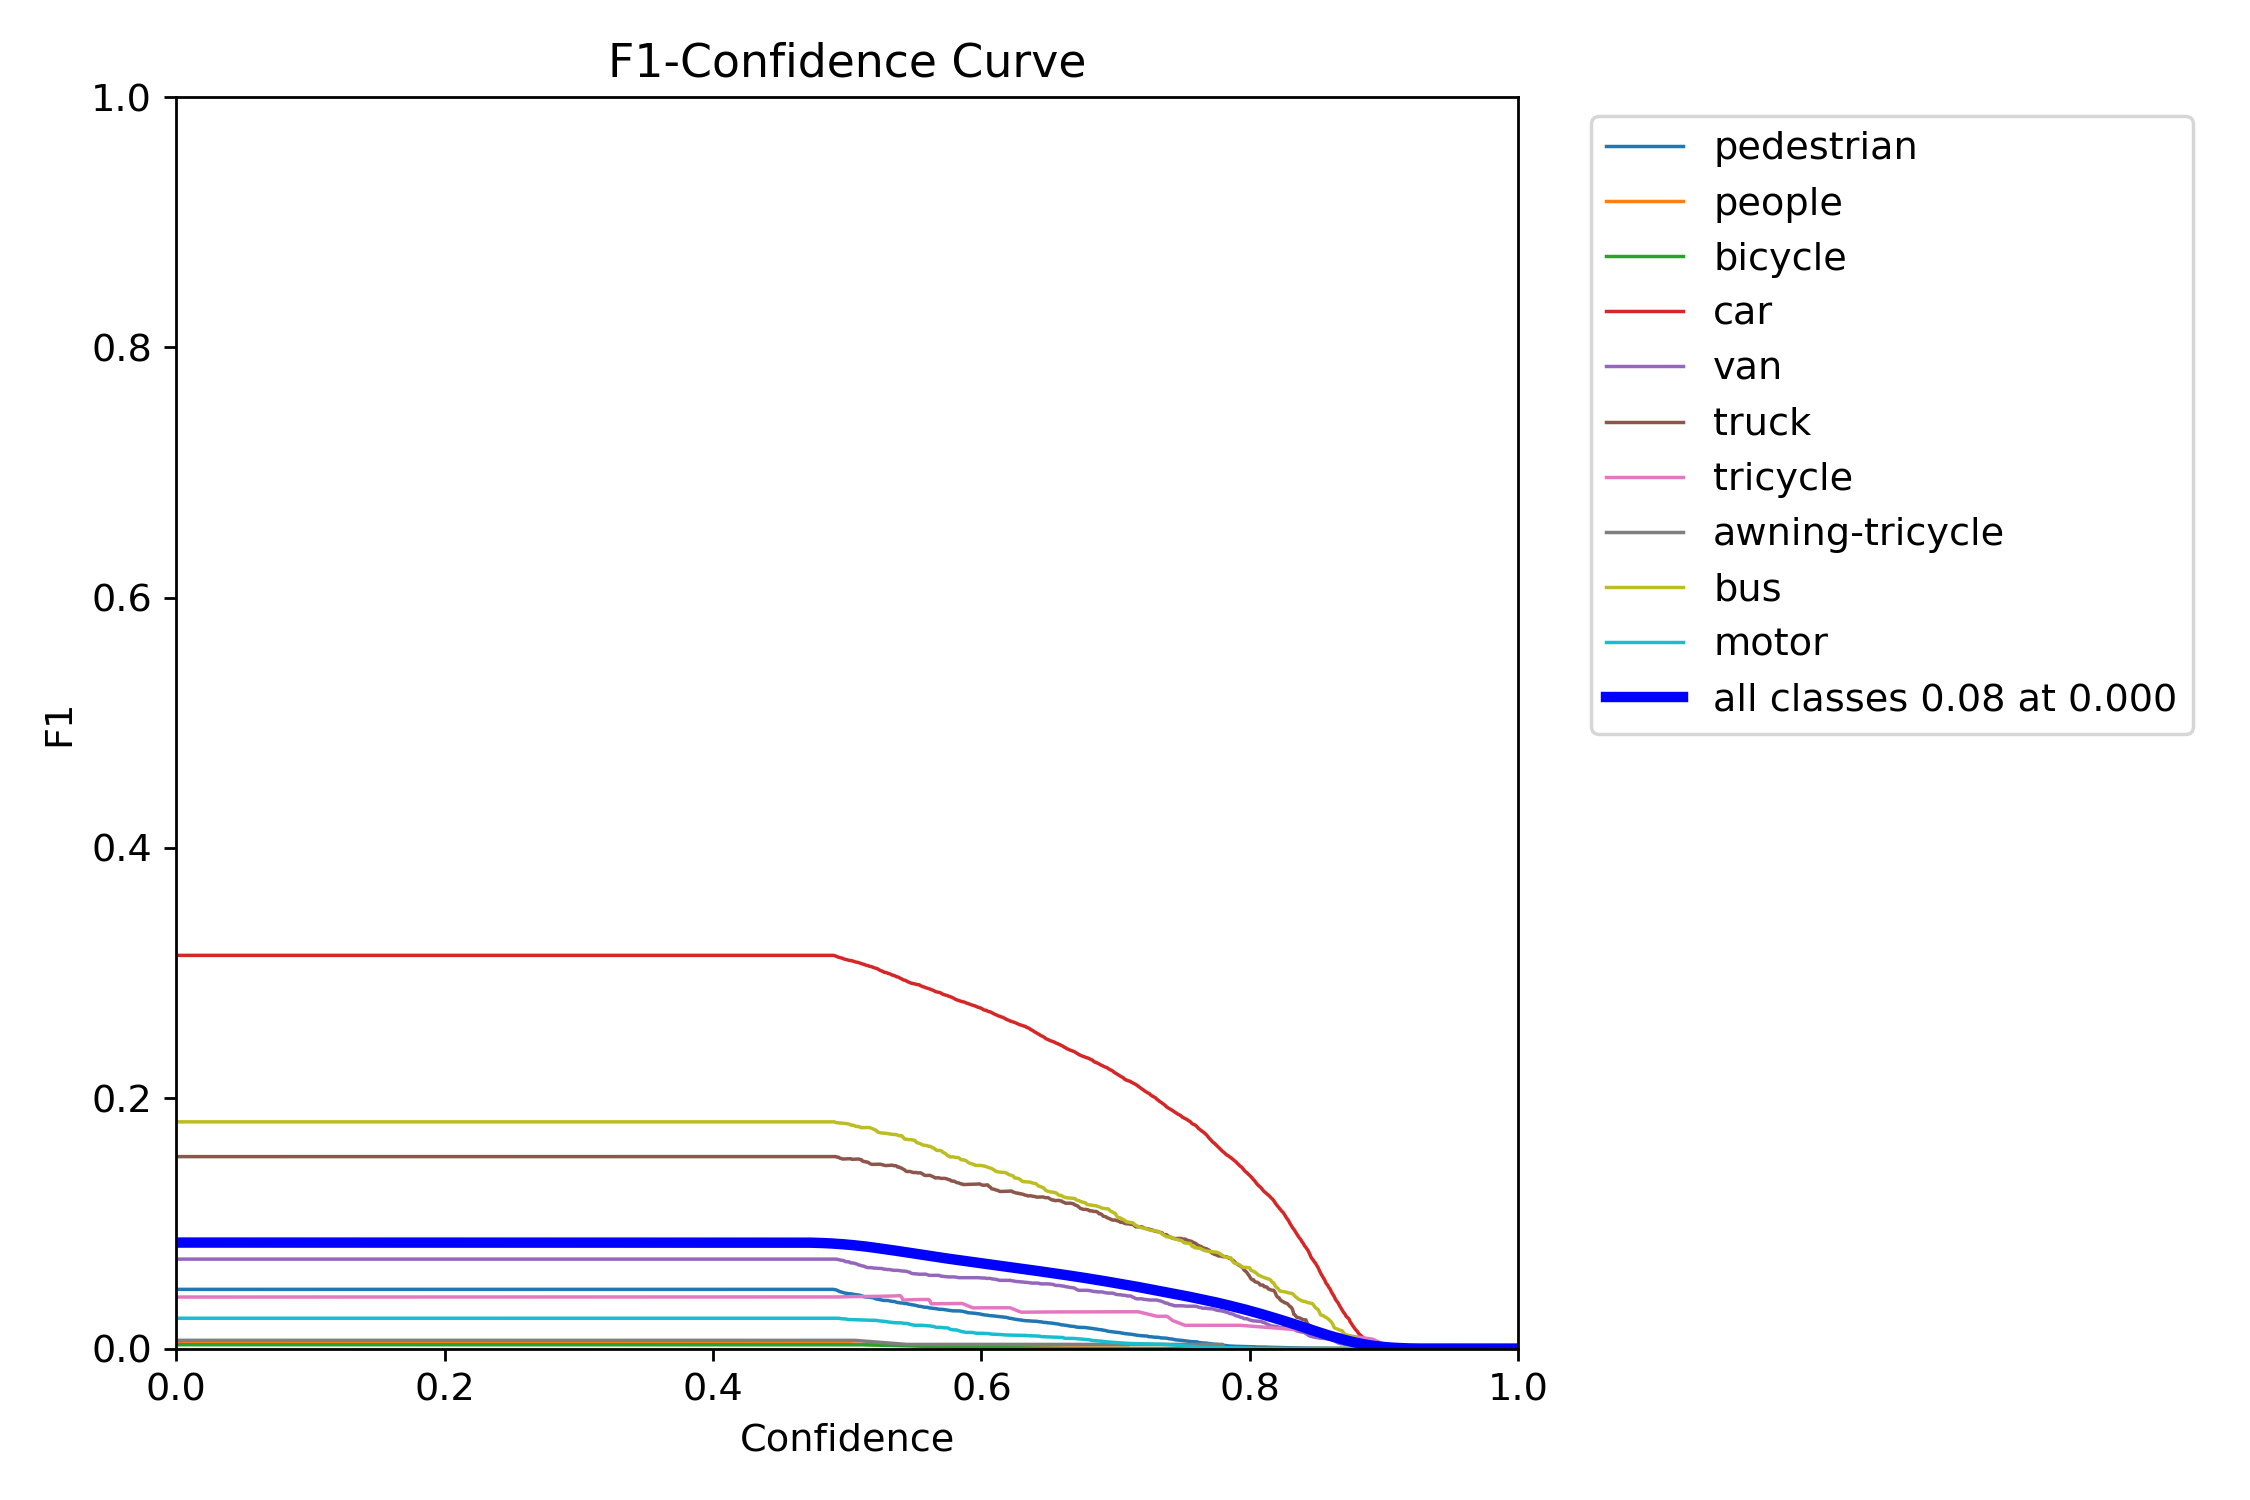
\includegraphics[width=0.4\textwidth]{../figure/fogvd_v11s_F1_curve.png}
    } \\
    \subfloat[YOLOv10s\label{fig:fogvd_10s_f1}]{
        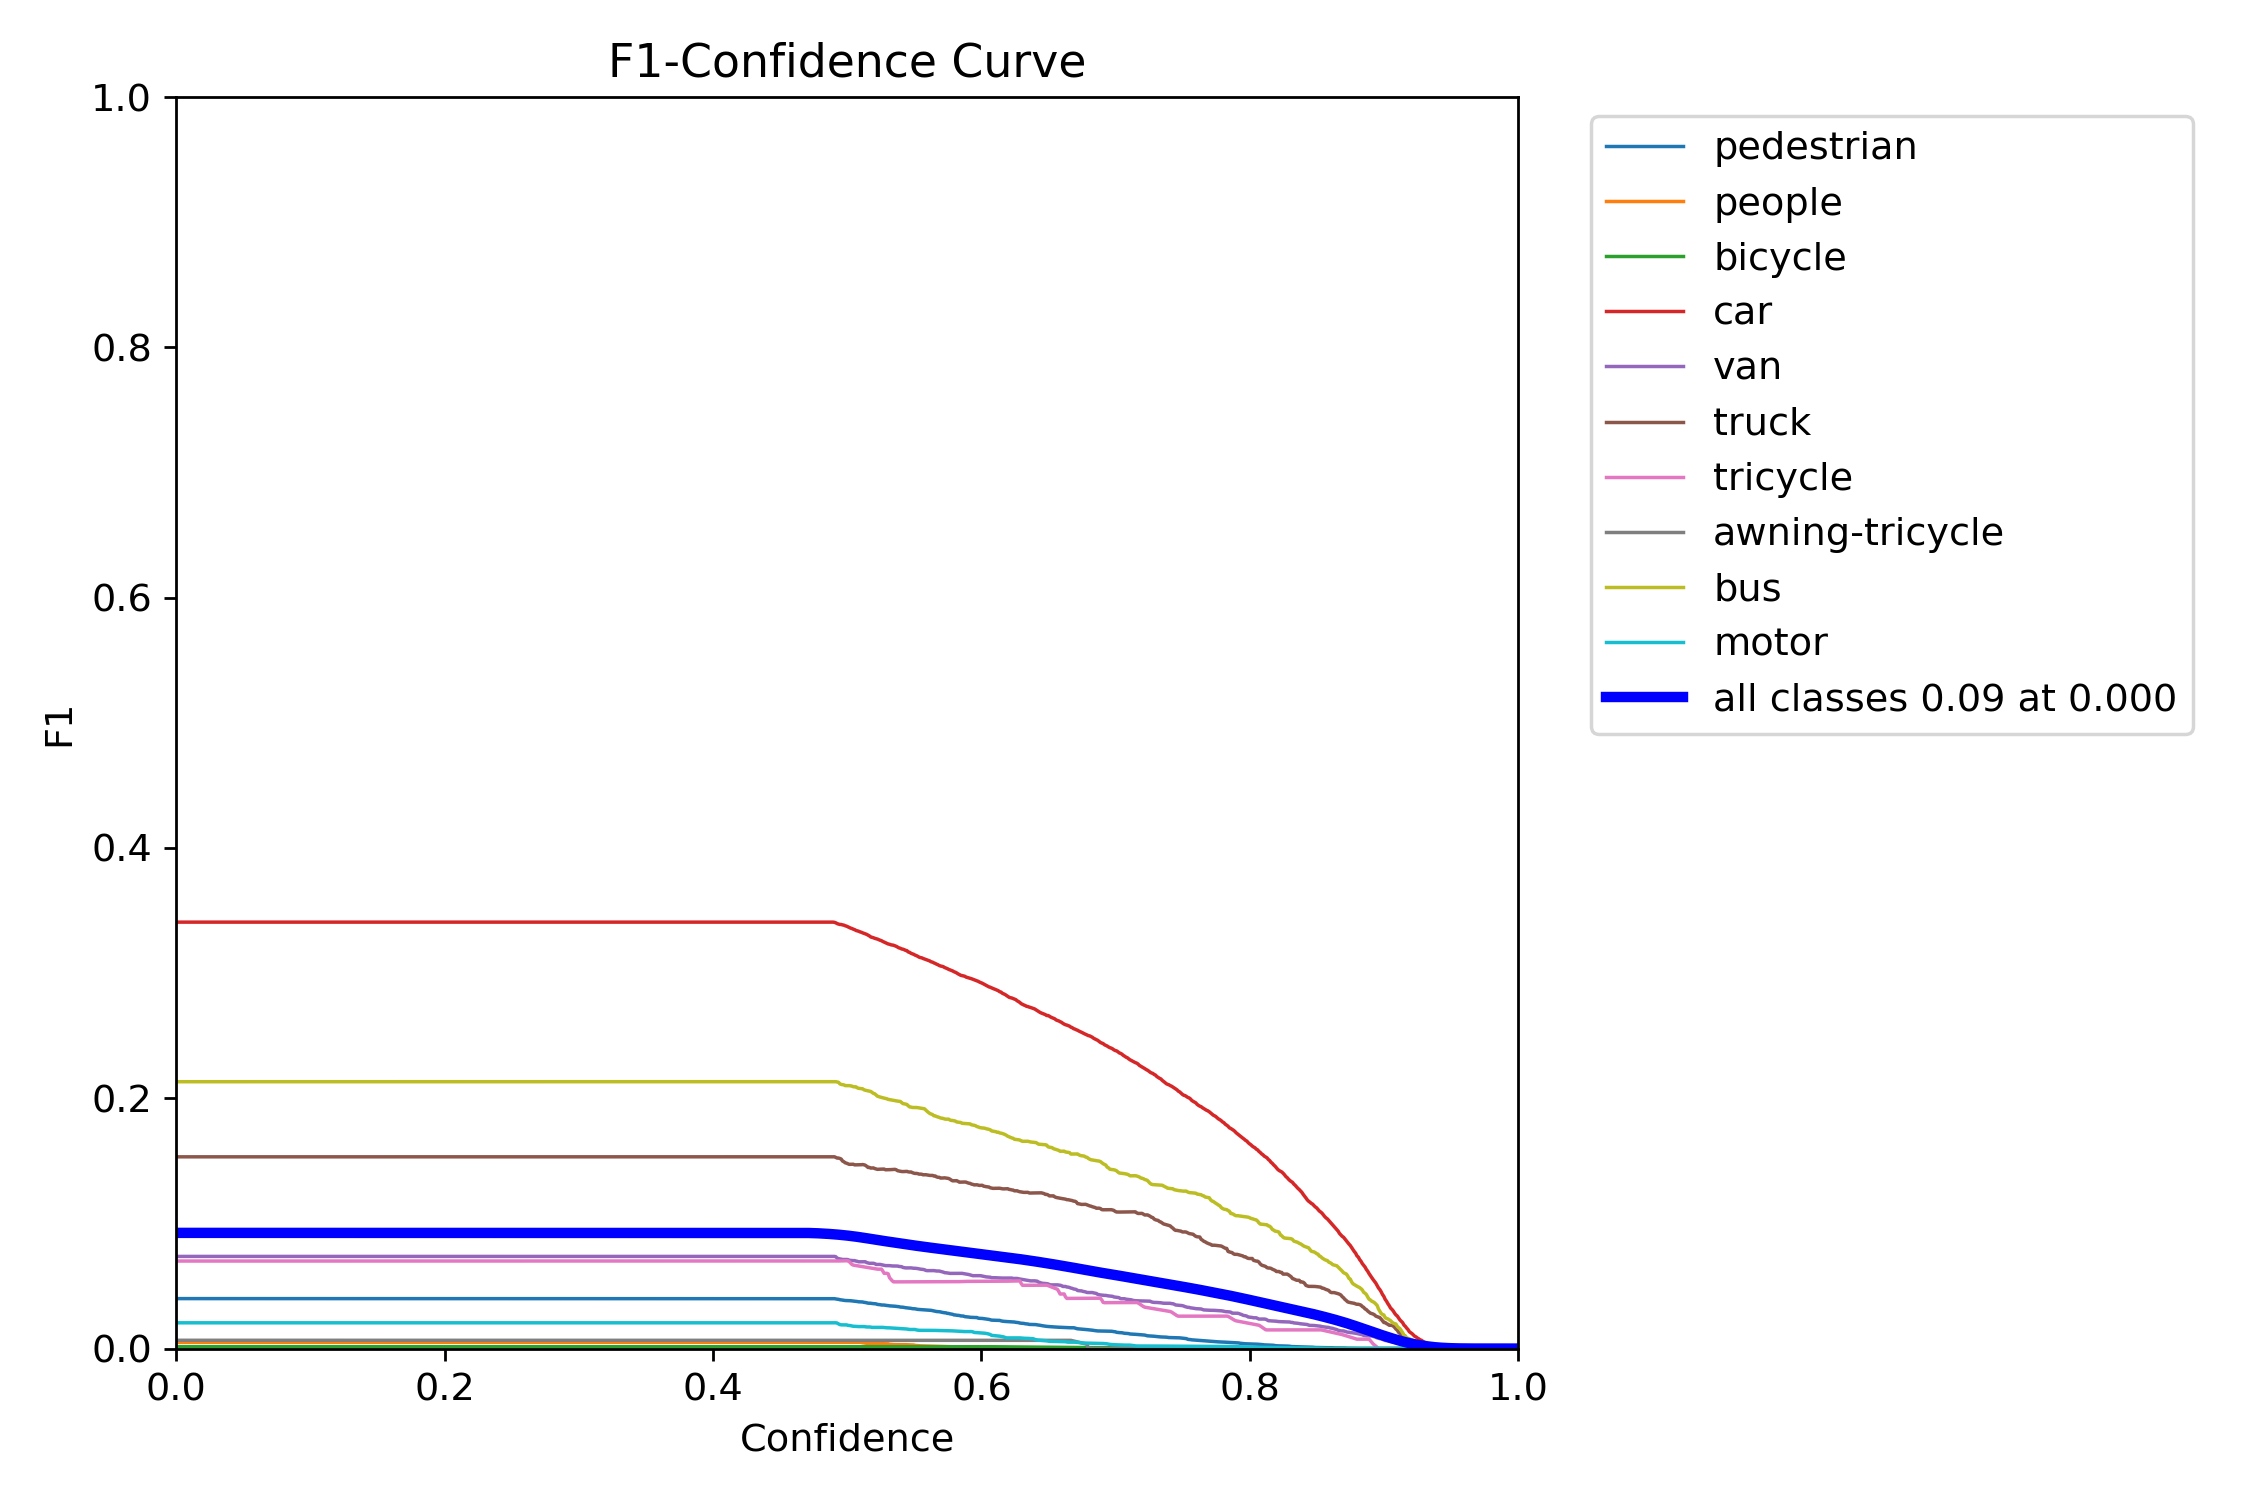
\includegraphics[width=0.4\textwidth]{../figure/fogvd_v10s_F1_curve.png}
    }
    \subfloat[YOLOv9s\label{fig:fogvd_9s_f1}]{
        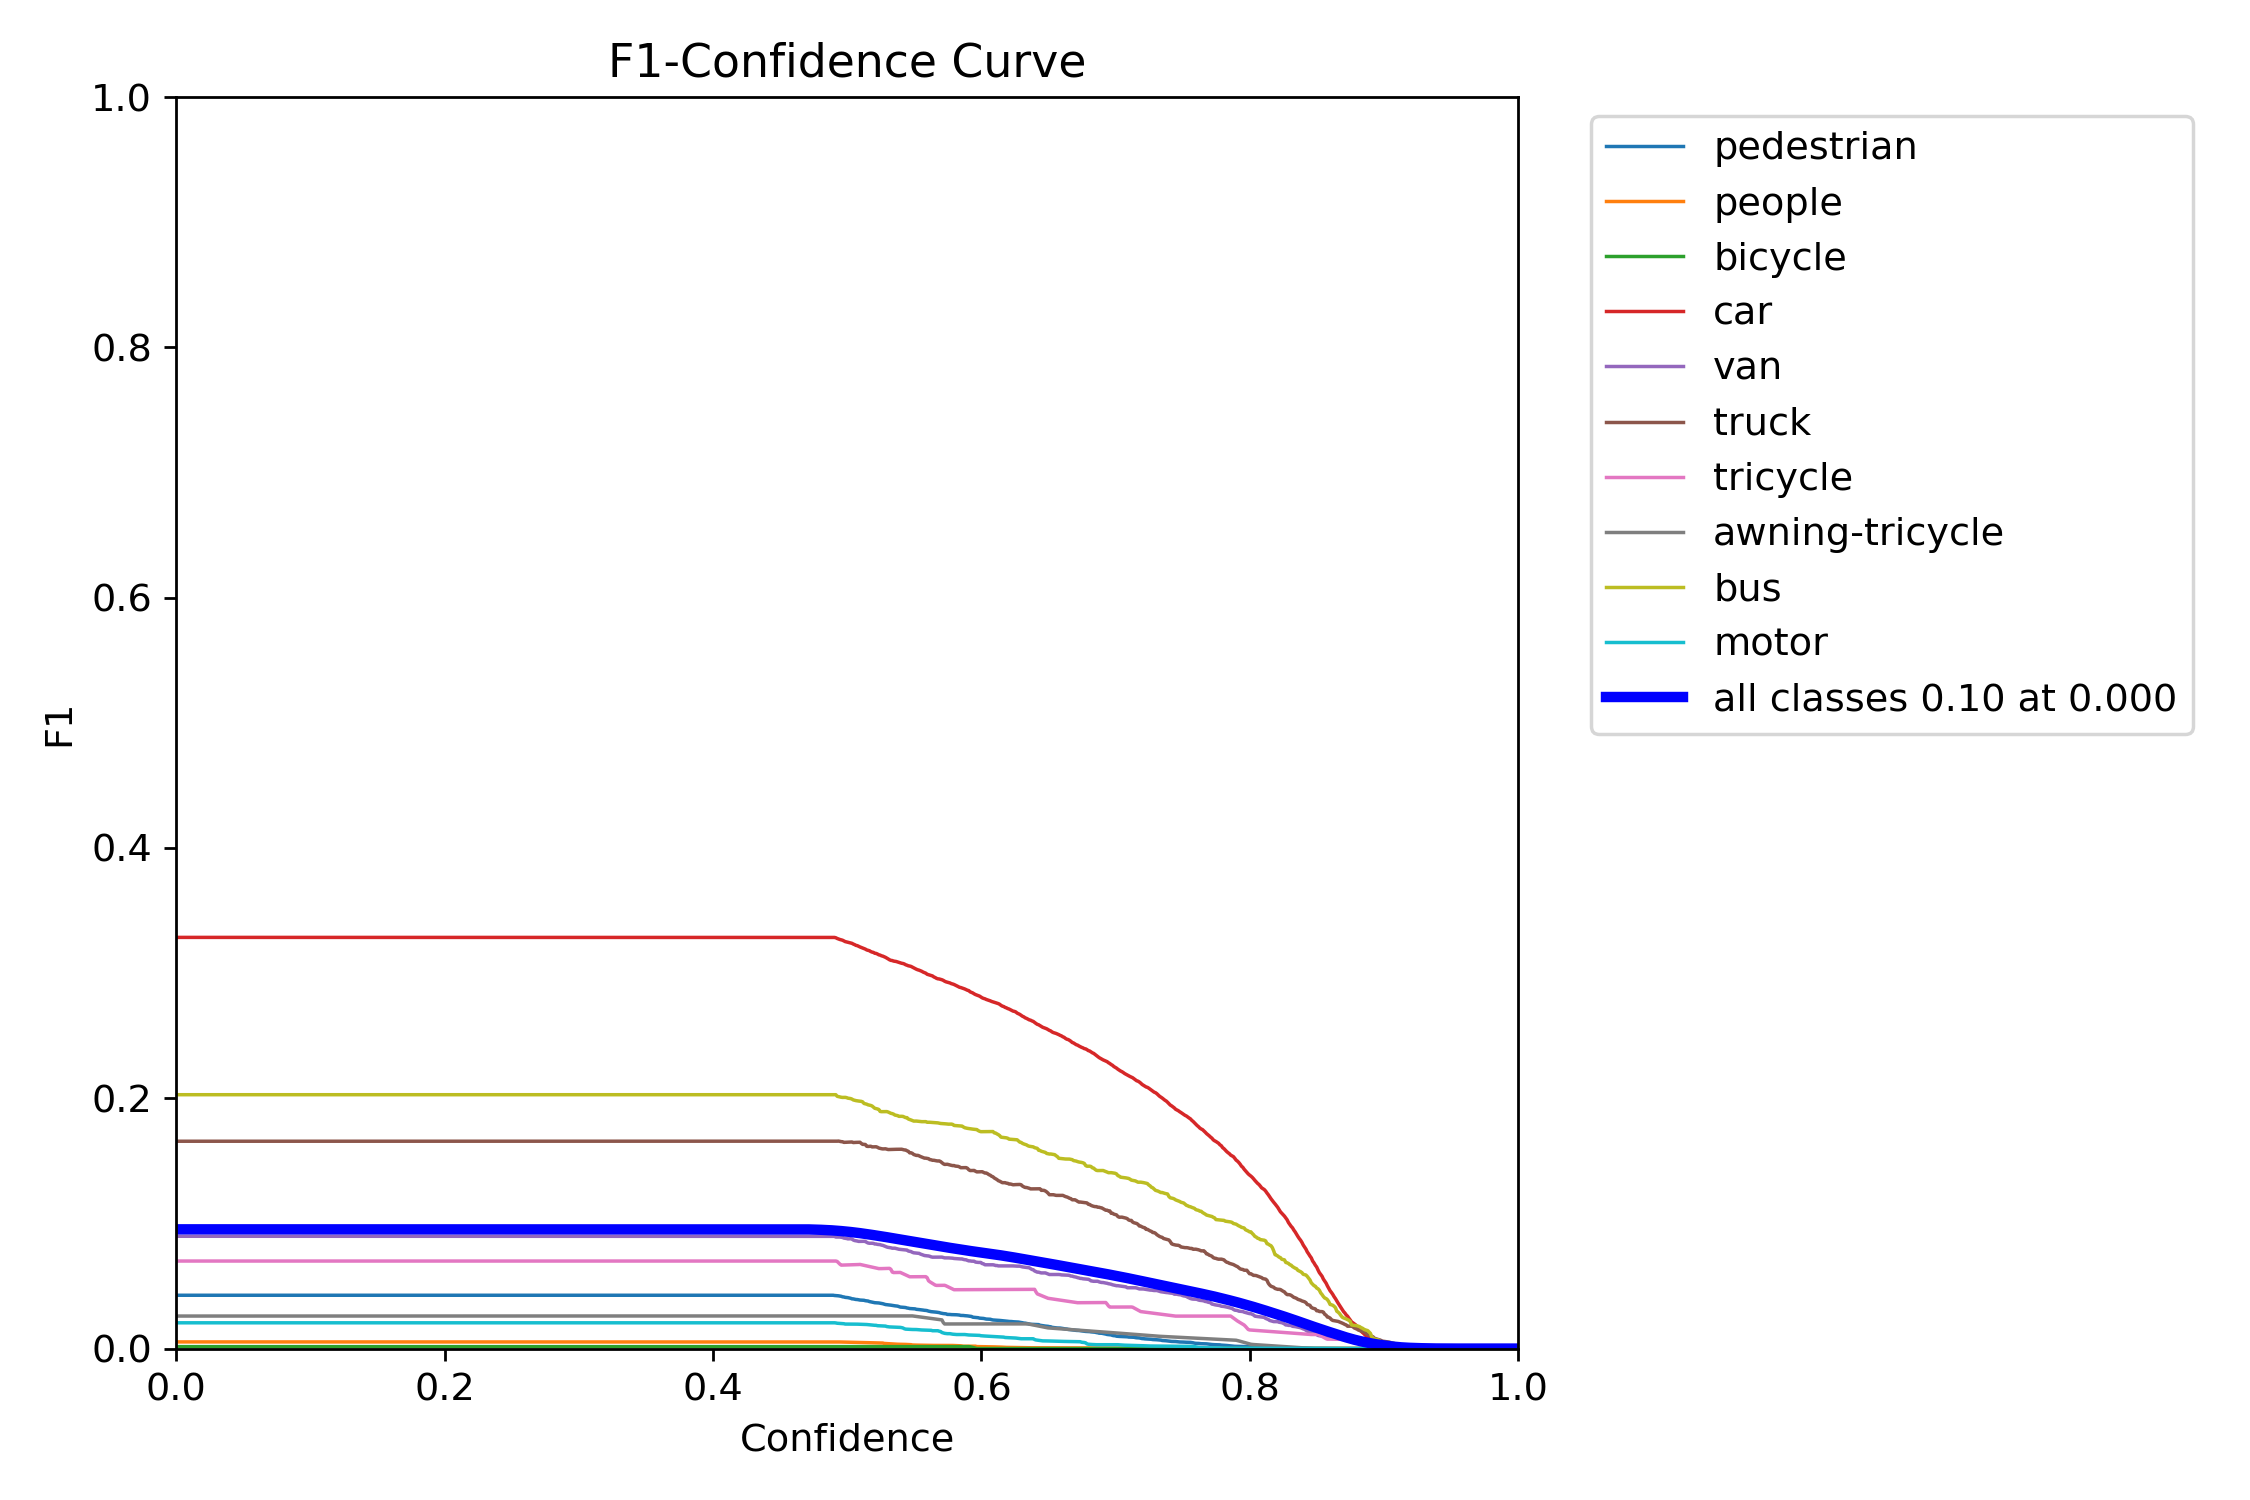
\includegraphics[width=0.4\textwidth]{../figure/fogvd_v9s_F1_curve.png}
    }
    \captionsetup{font=footnotesize}
    \bicaption{不同的网络模型在 FOG-VidDrone 数据集上的F1得分}{F1 scores of different network models on the FOG-VidDrone dataset.}
    \label{fig:fogvd_f1}
\end{figure}

在表 \ref{tab:compare_studies_fogvd} 中,从计算量(GFLOPs)来看,our 模型以 15.4 GFLOPs 显著低于 YOLOv11s(21.3 GFLOPs)、YOLOv10s(24.5 GFLOPs)和 YOLOv9s(26.7 GFLOPs)。这表明改进后的算法在降低计算复杂度方面成效显著,有助于提升无人机在复杂雾天环境中的运行效率和图像处理速度。



在精确度(P)方面,our 模型达到 0.721,优于 YOLOv11s(0.631)、YOLOv10s(0.674)和 YOLOv9s(0.642),展现出更高的目标检测精准性。
从召回率(R)来看,our 模型为 0.074,虽然数值较低,但已超出 YOLOv11s(0.049)、YOLOv10s(0.054)和 YOLOv9s(0.055),说明其在雾天场景下对交通目标的检测范围更广。



图 \ref{fig:fogvd_cmn} 展示了 YOLOv9s、YOLOv10s、YOLOv11s 以及 our 模型在 VisDrone 数据集针对不同类别目标的预测状况,以归一化混淆矩阵热力图形式呈现。热力图颜色深浅与预测概率正相关,颜色愈深表示预测准确率愈高,颜色愈浅则表明预测准确率较低。对角线数据反映模型成功预测正确标签的情况,非对角线数据则体现模型标签预测错误的情形。



从图 \ref{fig:fogvd_ex_cmn} 至图 \ref{fig:fogvd_9s_cmn} 可见,各模型在不同类别上的预测表现存在差异。
综合归一化混淆矩阵热力图信息可知,在 VisDrone 数据集上,YOLOv9s 模型在预测正确类别方面表现较为出色,这一结论与表 \ref{tab:compare_studies_fogvd} 中的数据相呼应 —— YOLOv9s 的精确度(0.525)和召回率(0.392)均处于较高水平。our 模型的精确度(0.514)略低于 YOLOv9s,但召回率(0.372)与 YOLOv11s(召回率 0.381)和 YOLOv10s(召回率 0.380)相近,整体性能优于 YOLOv10s 模型。尽管 our 模型在精确度和召回率上未超越 YOLOv9s,但其在特定类别预测上展现出独特优势,例如在 “pedestrian” 和 “awning-tricycle”类别预测中,our 模型的准确率达到了 0.35 和 0.13,相较于其他模型具有一定的竞争力。



在关键的 mAP 性能指标上,our 模型以 0.397 的 $mAP_{0.5}$ 领先于 YOLOv11s(0.339)、YOLOv10s(0.364)和 YOLOv9s(0.348)。这表明 our 模型在平衡精确度与召回率方面优势明显,在 FOG-VisDrone 数据集的复杂雾天交通场景目标检测任务中具有较强的竞争力。



综合来看,our 模型在 FOG-VisDrone 数据集上的表现全面优于对比的 YOLO 系列模型。其在保持较低计算量的同时,实现了更高的精确度、召回率和 mAP,有效解决了无人机在雾天环境下交通目标检测的难点问题。这种性能优势使其在实际应用中能够更加快速、准确地识别各类交通目标,对于提升无人驾驶飞行器在复杂气象条件下的检测性能和应用价值具有重要意义。

为了直观地看到 CGF-YOLO 的检测效果,选择了多组复杂的场景图进行测试。 使用 CGF-YOLO、YOLOv11s、YOLOv10s和 YOLOv9s 的加权文件被保留并用于测试和比较。 图像选择标准包括具有不同尺寸和重叠目标的复杂场景。 基于上述要求,可以清楚地看到 CGF-YOLO、YOLOv11s、YOLOv10s和YOLOv9s之间的差异。 其中,图\ref{fig:fogtt_1}显示了与数量少的小目标分布在图片边缘的复杂场景的比较,图\ref{fig:fogvd_1}显示了与密集小目标和不同类别的复杂场景的比较。

\begin{figure}[H]
    \centering
        \subfloat[FOG-TT100K 原图 \label{fig:fogtt_show_1}]{
            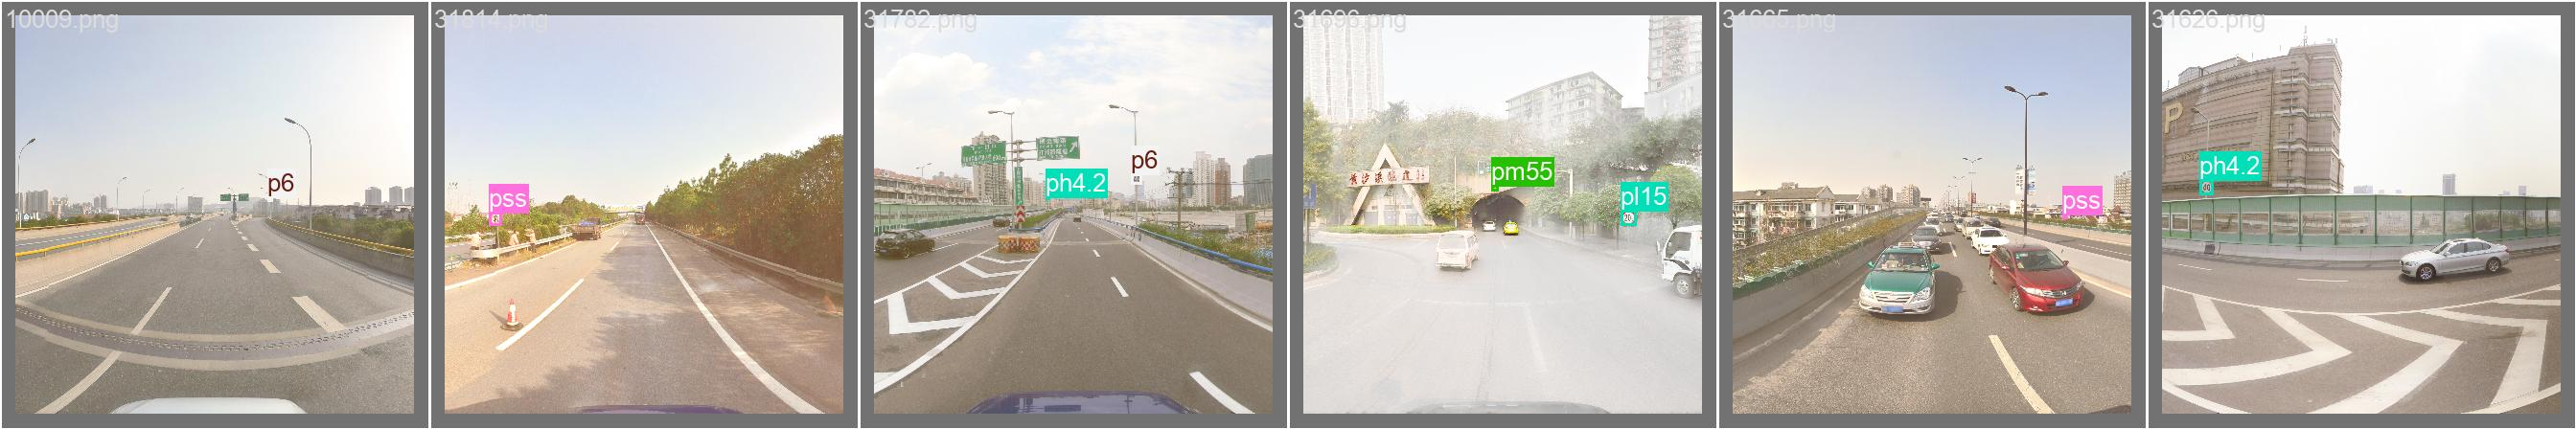
\includegraphics[width=0.95\textwidth]{../figure/tt_0_0.png}
        }
        \\
        \subfloat[CGF-YOLO \label{fig:fogtt_ex_1}]{
            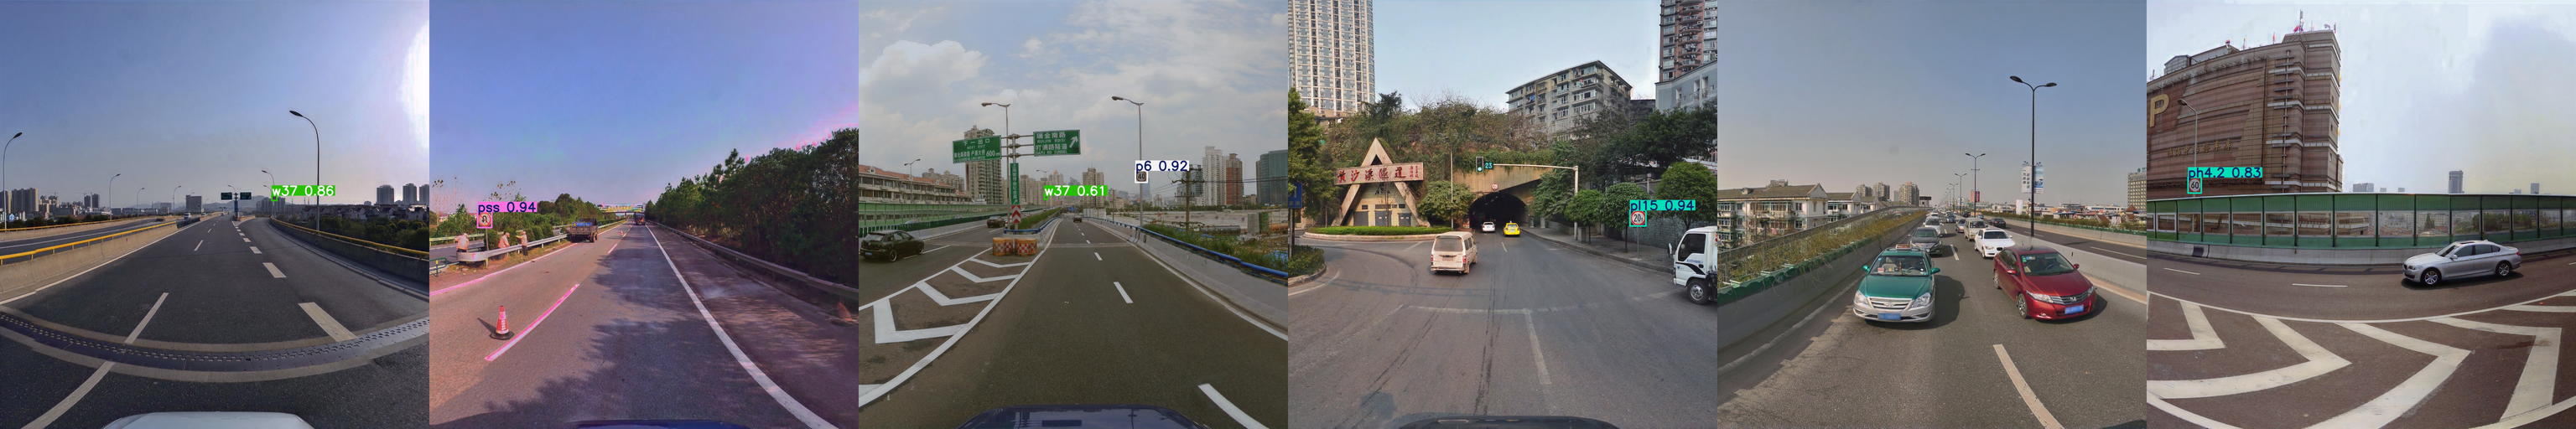
\includegraphics[width=0.95\textwidth]{../figure/fogtt_0_0_ex.png}
        }
        \\
        \subfloat[YOLOv11s \label{fig:fogtt_11s_1}]{
            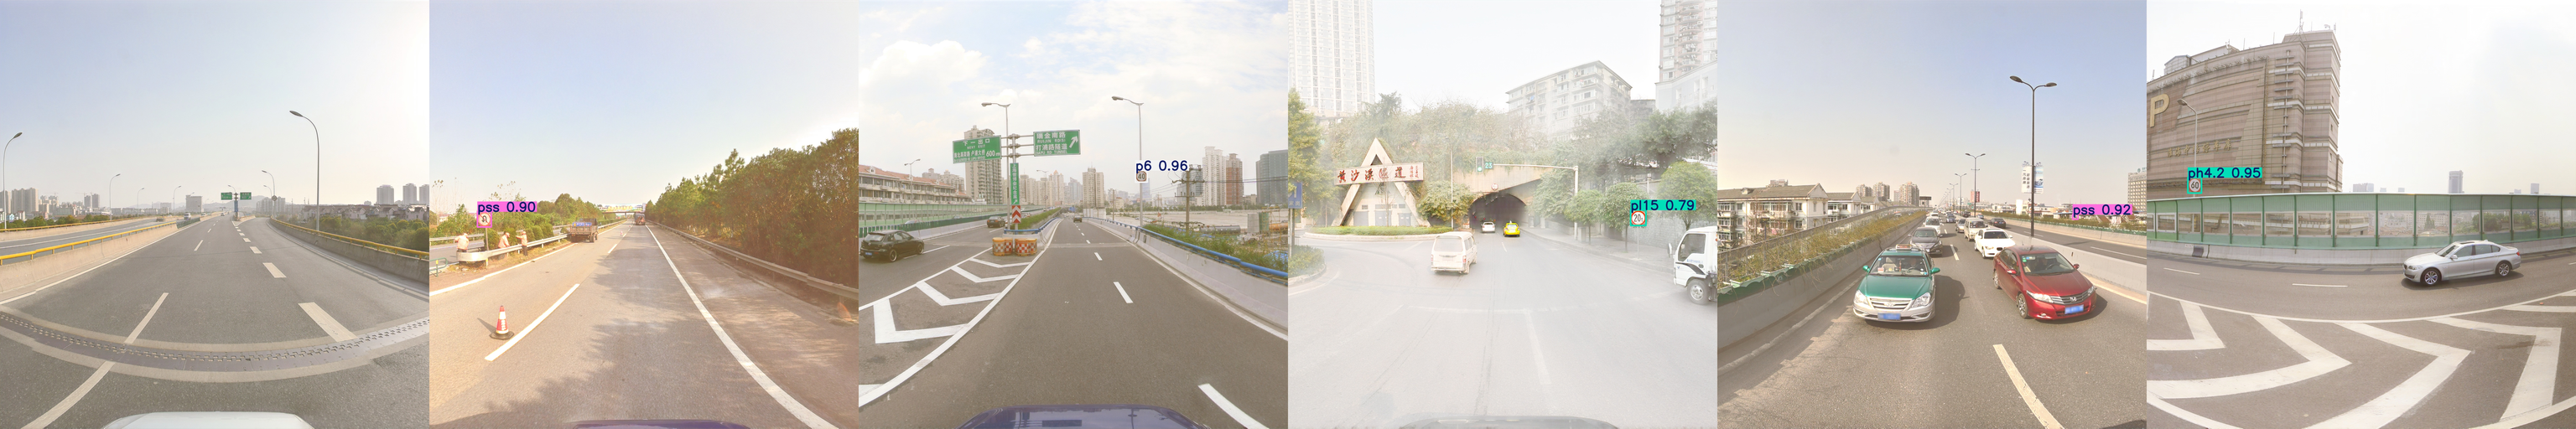
\includegraphics[width=0.95\textwidth]{../figure/fogtt_0_0_11.png}
        }
        \\
        \subfloat[YOLOv10s \label{fig:fogtt_10s_1}]{
            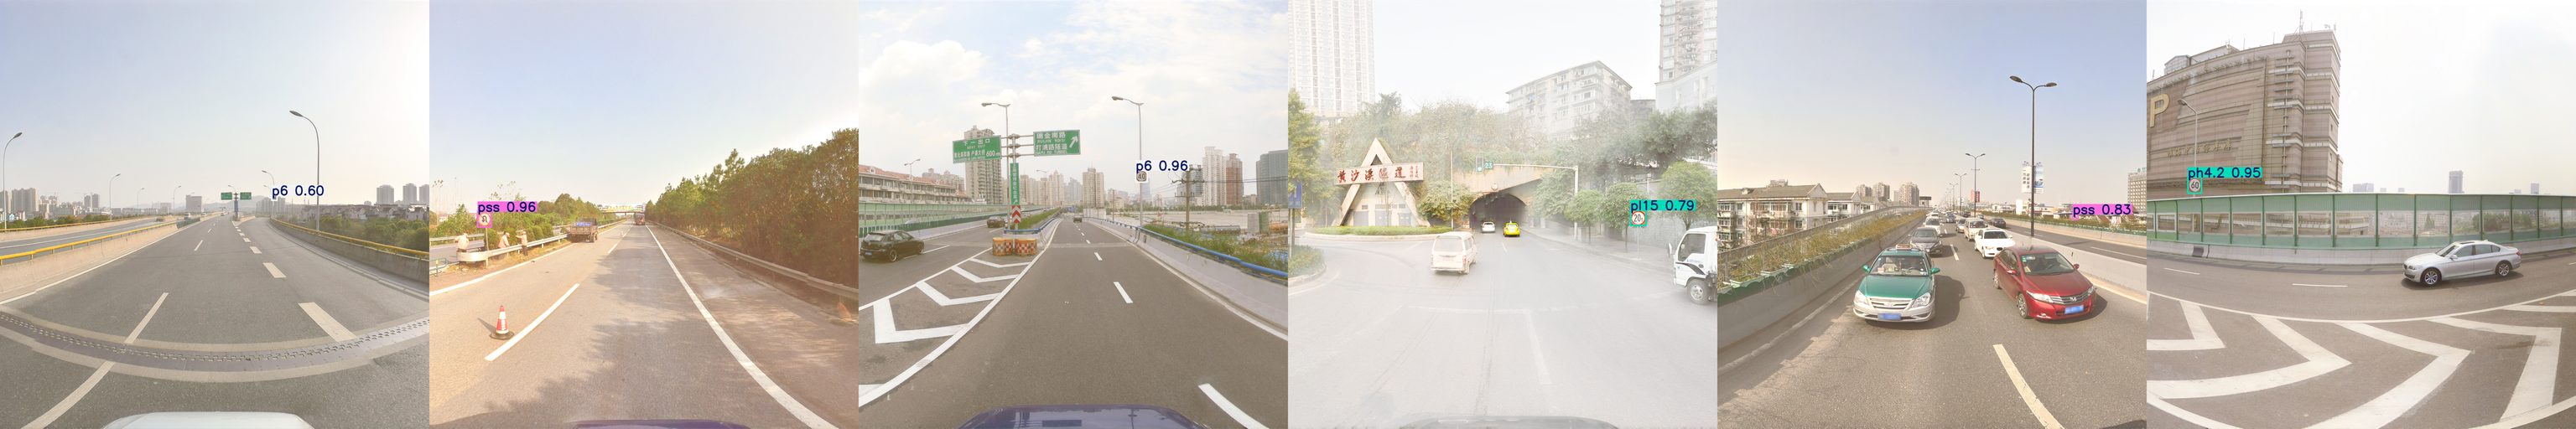
\includegraphics[width=0.95\textwidth]{../figure/fogtt_0_0_10.png}
        }
        \\
        \subfloat[YOLOv9s \label{fig:fogtt_9s_1}]{
            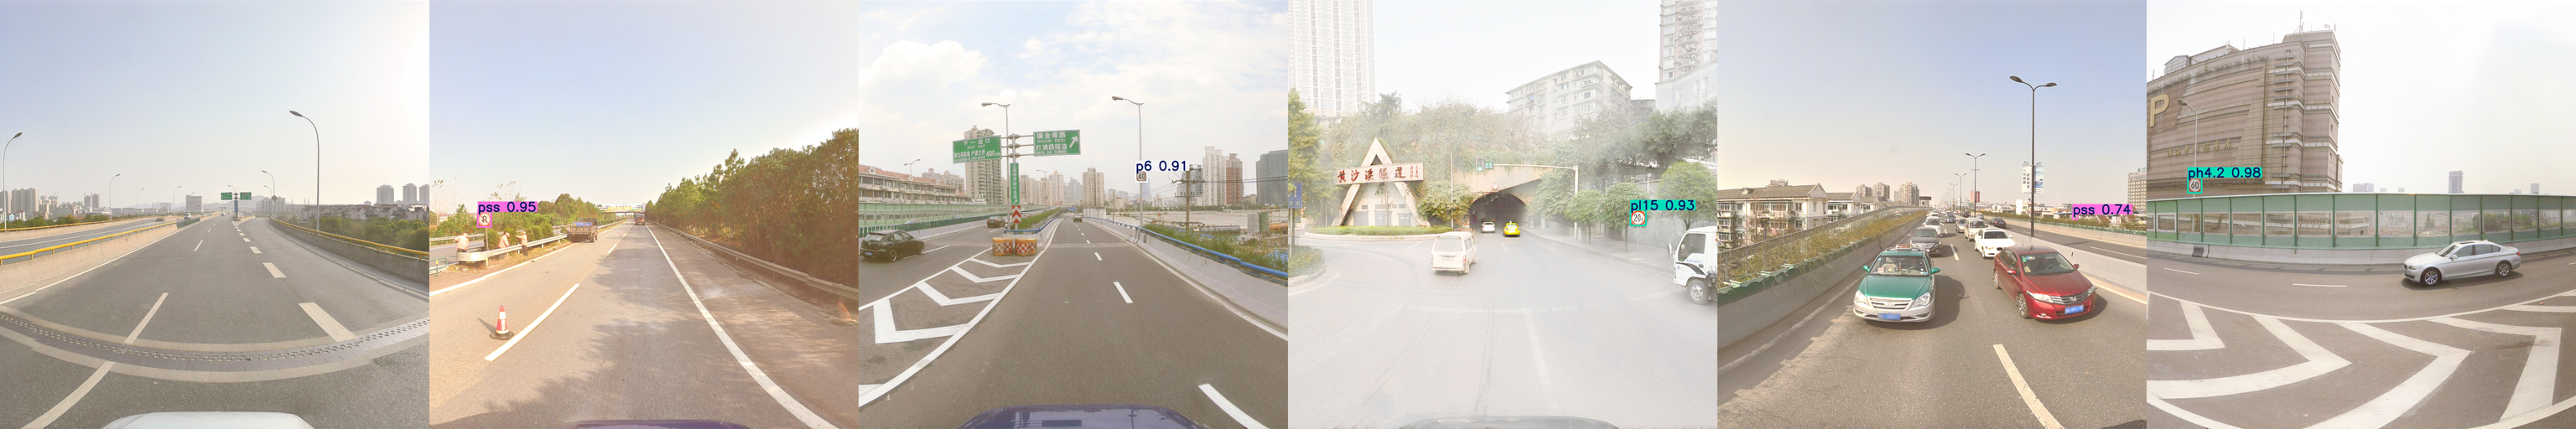
\includegraphics[width=0.95\textwidth]{../figure/fogtt_0_0_9.png}
        }
    \captionsetup{font=footnotesize}
    \bicaption{不同网络模型在 FOG-TT100K 数据集上的推理结果}{Symbol cross-reference table}
    \label{fig:fogtt_1}
\end{figure}

在图\ref{fig:fogtt_1}的比较实验中,选择了 FOG-TT100K 数据集中具有复杂场景和干扰的图像。
图\ref{fig:fogtt_1}显示,由于目标场景的复杂性,YOLOv9s无法检测到图片中的所有目标信息,YOLOv10s只能检测到一小部分目标信息,而YOLOv11s和CGF-YOLO检测到更完整的目标信息。 可以看出,YOLOv9和YOLOv10在检测小目标方面仍然存在一些问题。 相比之下,CGF-YOLO 可以用低计算能力准确检测正确的目标。

\begin{figure}[H]
    \centering
        \subfloat[FOG-VisDrone 原图 \label{fig:fogvd_show_1}]{
            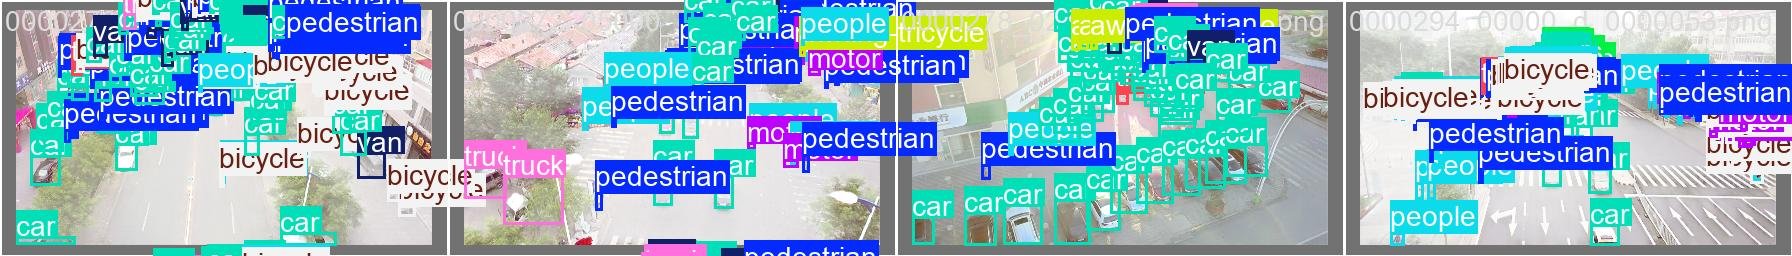
\includegraphics[width=1.0\textwidth]{../figure/vd_0_1.png}
        }
        \\
        \subfloat[CGF-YOLO \label{fig:fogvd_ex_1}]{
            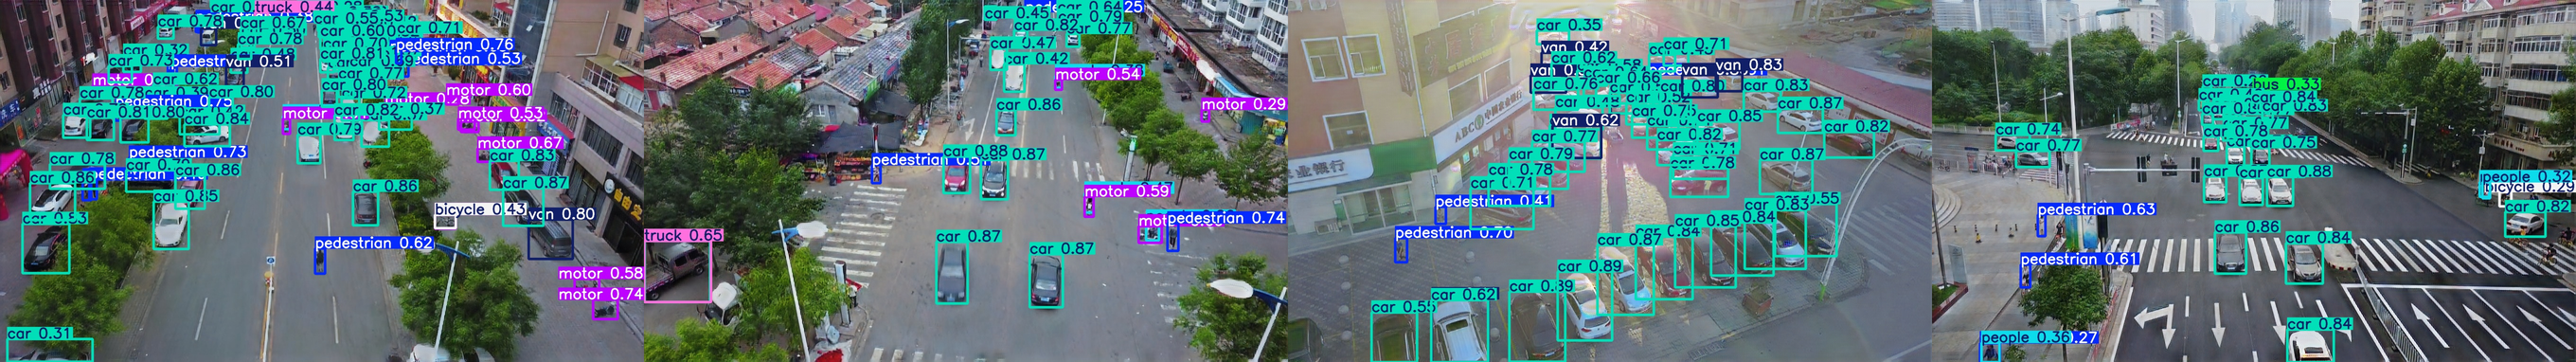
\includegraphics[width=1.0\textwidth]{../figure/vd_0_1_ex.png}
        }
        \\
        \subfloat[YOLOv11s \label{fig:fogvd_11s_1}]{
            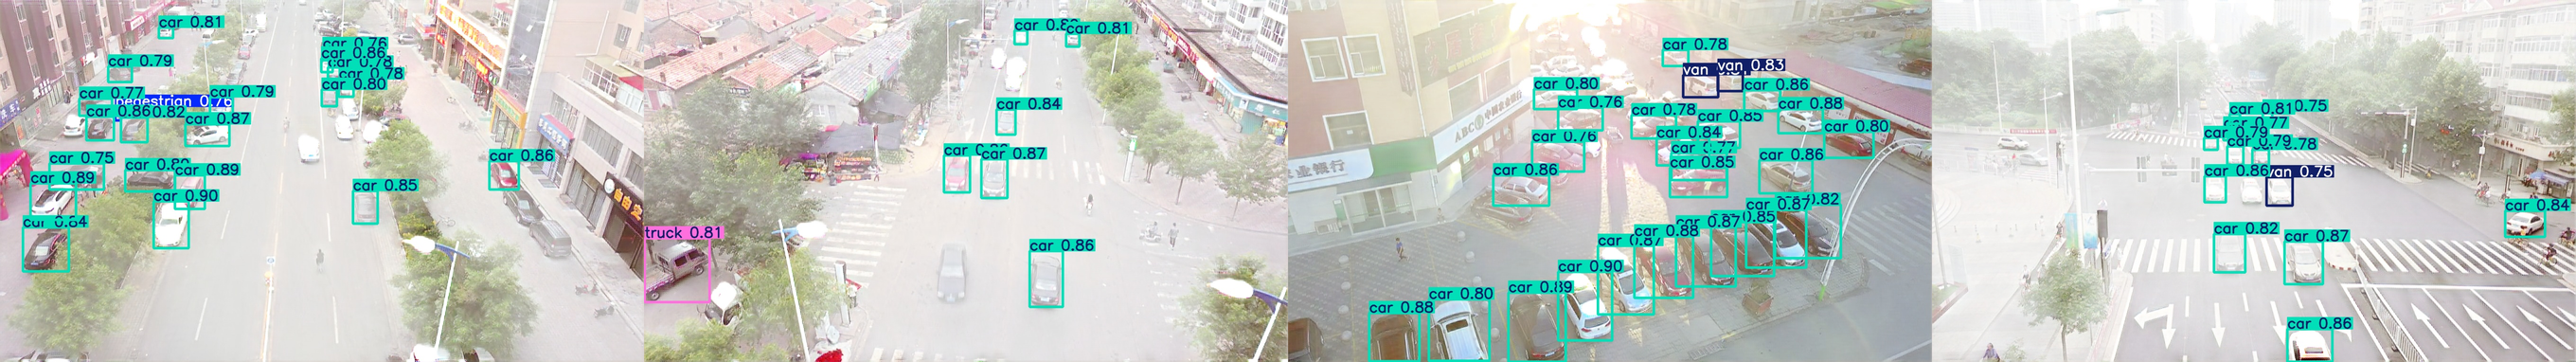
\includegraphics[width=1.0\textwidth]{../figure/vd_0_1_11.png}
        }
        \\
        \subfloat[YOLOv10s \label{fig:fogvd_10s_1}]{
            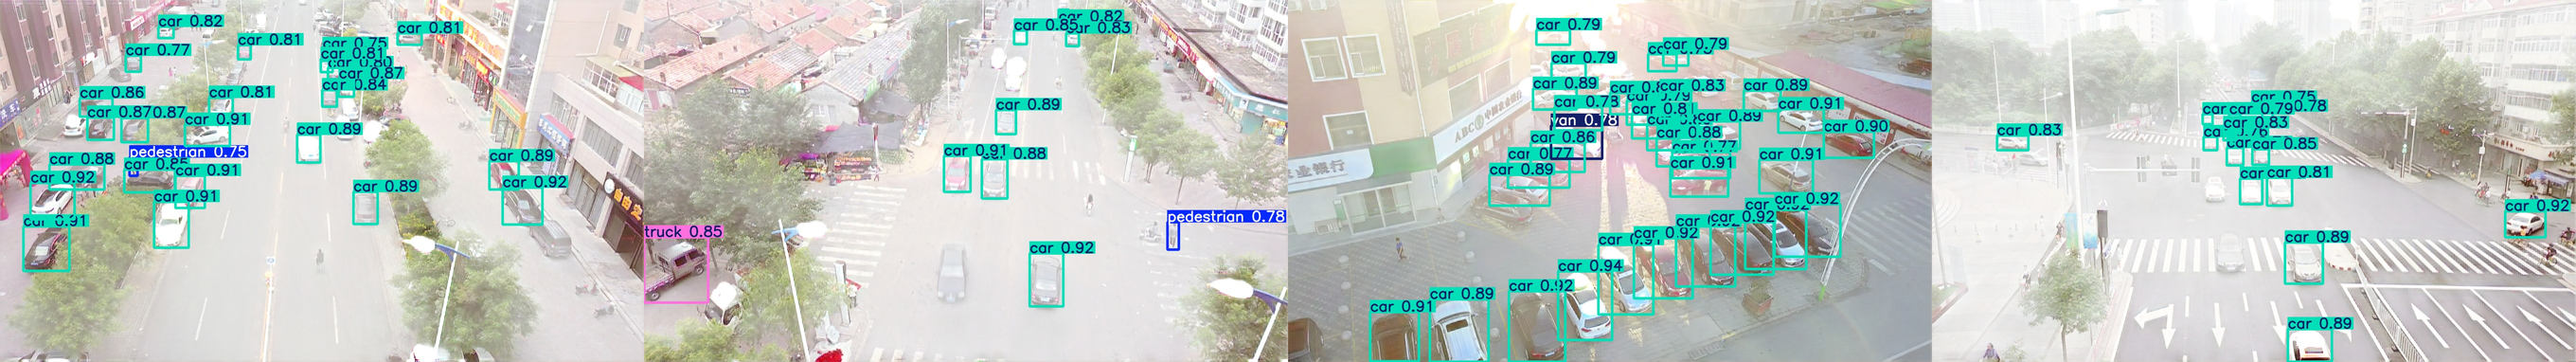
\includegraphics[width=1.0\textwidth]{../figure/vd_0_1_10.png}
        }
        \\
        \subfloat[YOLOv9s \label{fig:fogvd_9s_1}]{
            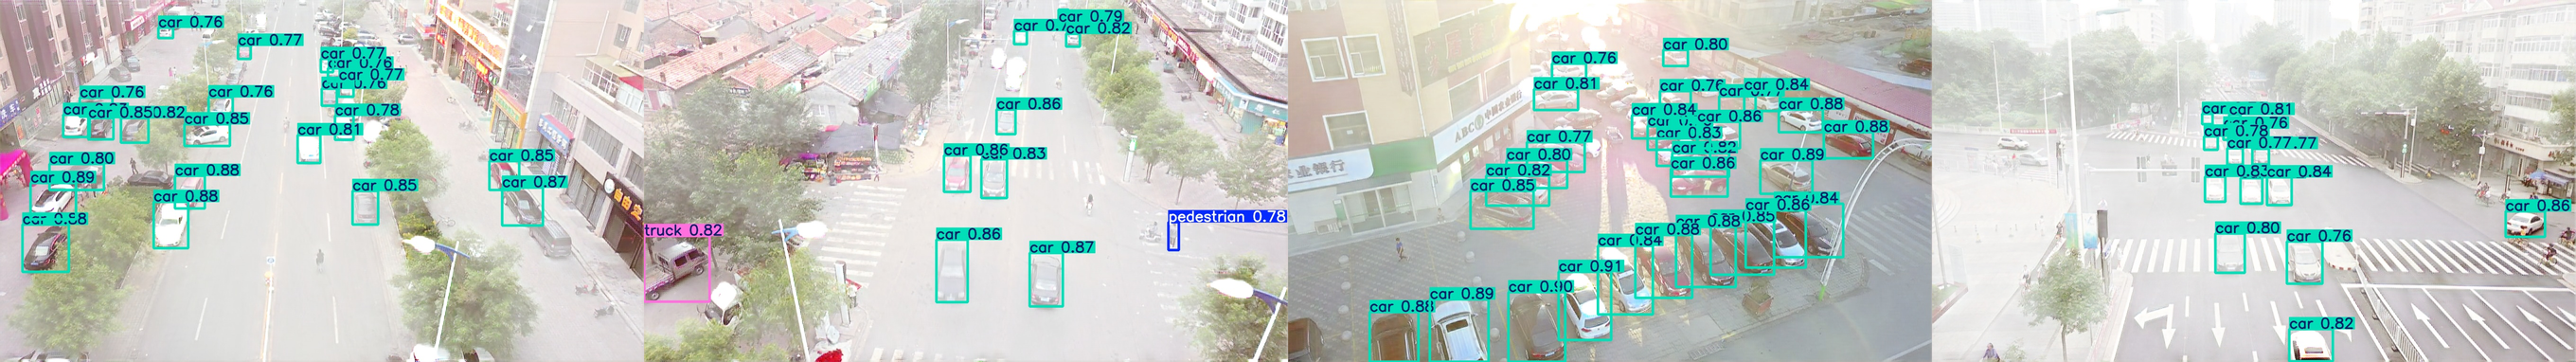
\includegraphics[width=1.0\textwidth]{../figure/vd_0_1_9.png}
        }
    \captionsetup{font=footnotesize}
    \bicaption{不同网络模型在 FOG-VisDrone 数据集上的推理结果}{Symbol cross-reference table}
    \label{fig:fogvd_1}
\end{figure}

在图 \ref{fig:fogvd_1} 的比较实验中,在VisDrone数据集中选择具有复杂场景、小而密集的目标、各种目标、模糊和干扰的图像。
在图 \ref{fig:fogvd_1} 中,所有模型的探测器都无法检测到所有检测目标,只能检测其中的一部分。 可以看出,YOLOv9s表现最好,这与其高mAP相吻合。 YOLOv10s和YOLOv11s在检测具有各种目标、模糊和干扰的小型密集目标方面仍然没有足够的性能。 相比之下,CGF-YOLO可以在低计算量下准确检测更准确的目标,显示出接近YOLOv9s的检测性能,并且可以在复杂和重叠的场景中准确检测更多目标。 从图 \ref{fig:fogvd_1} 可以看出,CGF-YOLO的检测性能明显优于YOLOv10s和YOLOv11s,但略低于YOLOv9s。



根据图 \ref{fig:fogtt_1}、图 \ref{fig:fogvd_1},当目标分布不均匀且分布不密集时,YOLOv11s可以实现更好的识别性能,而YOLOv9s可以在目标分布密集的条件下正确捕获更多目标。 CGF-YOLO可以平衡这两种情况,以实现尽可能高的识别性能,这显然优于YOLOv10s,CGF-YOLO大大减少了计算量。 这有利于无人机在面对复杂场景时识别小目标。

\subsection{本章小结}

综上所述,本章基于 CycleGAN 网络提出了一种改进的去雾还原算法。首先,对原始 CycleGAN 网络的生成器和判别器进行了详细分析,并结合其在图像去雾还原任务中的优势与局限性,针对性地进行了改进。在生成器网络中,将 Transformer 模块与 ResNet 残差块结构相结合,充分利用了 Transformer 的自注意力机制来捕捉图像的全局依赖关系,突破了传统卷积操作局部感受野的限制,从而能够更精准地还原雾天图像中的细节信息,如物体边缘和纹理等。判别器网络则采用了局部-全局结合的架构,局部判别器聚焦于图像细节特征,确保生成图像在局部区域的纹理和结构真实性;全局判别器则从整体上把控图像的宏观特征和风格,使去雾后的图像在整体布局、颜色分布等方面更符合清晰图像的要求。

为了验证改进算法的有效性,本章在 FOG-TT100K 和 FOG-VisDrone 数据集上进行了图像去雾实验和雾天目标检测实验,并与 YOLOv9s、YOLOv10s、YOLOv11s 等先进算法进行了对比分析。实验结果表明,改进后的算法在精确度、召回率和 mAP 等指标上均优于对比算法,同时在计算量上也显著降低,展现出较低的计算复杂度,这使得该算法在无人机等资源受限的设备上具有较高的实际应用价值,能够有效提升其在复杂雾天场景下对交通目标的检测效率和实用性。总体而言,本章提出的基于改进 CycleGAN 网络的去雾还原算法在提升去雾图像质量、增强后续雾天目标检测性能以及降低计算成本等方面均取得了显著成果,为雾天图像处理和目标检测领域提供了新的思路和方法,但仍然存在一些局限性,如在部分场景下召回率有待进一步提高等,这也将是未来研究工作的重要方向之一。
